\documentclass{dissertation-edit}

%%% My own packages
\usepackage{graphicx}% Include figure files
\usepackage{dcolumn}% Align table columns on decimal point
\usepackage{bm}% bold math
\usepackage{hyperref}% add hypertext capabilities
%\usepackage[mathlines]{lineno}% Enable numbering of text and display math
%\linenumbers\relax % Commence numbering lines
\usepackage{xcolor} % colored text
\usepackage{textcomp}
\usepackage[mode=text]{siunitx} % see https://tex.stackexchange.com/questions/423711/text-font-in-maths-mode-with-siunitx
\DeclareSIUnit{\sqrthz}{\ensuremath{\sqrt{\text{\hertz}}}}
%\sisetup{detect-all} % tell siunitx to use standard font, not math font
%\usepackage{float} % force figure placement
\usepackage{mathtools} % for defining my own math commands
\DeclarePairedDelimiter\abs{\lvert}{\rvert}
\usepackage{listings} % for code blocks
\usepackage{esdiff} % for easier typing out derivatives
\usepackage[version=4]{mhchem}
\usepackage{accents}
\usepackage{multirow}
\usepackage{tabularx}
\newcolumntype{Y}{>{\centering\arraybackslash}X} % automatic linebreak in tables, with centering
\usepackage{pdfpages}


\definecolor{dkgreen}{rgb}{0,0.6,0}
\definecolor{gray}{rgb}{0.5,0.5,0.5}
\definecolor{mauve}{rgb}{0.58,0,0.82}
\definecolor{skyblue}{rgb}{0.36,0.8,0.86}
\definecolor{darkgreen}{rgb}{0.18,0.54,0.34}
\definecolor{maroon}{rgb}{0.64,0.16,0.16}
\definecolor{darkpink}{rgb}{0.75,0.25,0.5}

\lstset{frame=single,
	language=[ISO]C++,
	aboveskip=3mm,
	belowskip=3mm,
	showstringspaces=false,
	columns=flexible,
%	basicstyle={\small\ttfamily},
	numbers=none,
	numberstyle=\color{gray},
%	keywordstyle=\color{blue},
%	commentstyle=\color{dkgreen},
%	stringstyle=\color{mauve},
	rulecolor=\color{black},
	breaklines=true,
	breakatwhitespace=true,
	tabsize=3,
	keywordstyle=\color{blue},
	commentstyle=\color{dkgreen},
	stringstyle=\color{mauve},
	basicstyle={\color{blue}\small\ttfamily},
	identifierstyle={\color{black}},
	literate=*
	{*}{{{\color{black}*}}}{1}
	{=}{{{\color{black}=}}}{1}
	{;}{{{\color{black};}}}{1}
	{.7}{{{\color{blue}.7}}}{2},
}
%\def\lst@visiblespace{\lst@ttfamily{\ }{\ }}
\usepackage{afterpage}
\usepackage{subcaption}
\renewcommand*{\thefootnote}{\arabic{footnote}}


\begin{document}

%% Specify the title and author of the thesis. This information will be used on the title page (in title/title.tex) and in the metadata of the final PDF.
\title[Fundamental studies and applications]{Josephson junctions in superconducting coplanar DC bias cavities}
\author{Felix Erik}{Schmidt}

%% Use Roman numerals for the page numbers of the title pages and table of contents.
%\frontmatter % !! Leave commented out, otherwise there will be a "0" thumb at some point (I think?)
%
%\begin{titlepage}

\begin{center}

%% Extra whitespace at the top.
\vspace*{2\bigskipamount}

%% Print the title.
{\makeatletter
\titlestyle\bfseries\LARGE\@title
\makeatother}

%% Print the optional subtitle.
{\makeatletter
\ifx\@subtitle\undefined\else
    \bigskip
    \titlefont\titleshape\Large\@subtitle
\fi
\makeatother}

\end{center}

\cleardoublepage
\thispagestyle{empty}

\begin{center}

%% The following lines repeat the previous page exactly.

\vspace*{2\bigskipamount}

%% Print the title.
{\makeatletter
\titlestyle\bfseries\LARGE\@title
\makeatother}

%% Print the optional subtitle.
{\makeatletter
\ifx\@subtitle\undefined\else
    \bigskip
    \titlefont\titleshape\Large\@subtitle
\fi
\makeatother}

%% Uncomment the following lines to insert a vertically centered picture into
%% the title page.
%\vfill
%\includegraphics{title}
\vfill

%% Apart from the names and dates, the following text is dictated by the
%% promotieregelement.

{\Large\titlefont\bfseries Dissertation}

\bigskip
\bigskip

for the purpose of obtaining the degree of doctor

at Delft University of Technology

by the authority of the Rector Magnificus, prof.dr.ir. T.H.J.J. van der Hagen

chair of the Board for Doctorates

to be defended publicly on

[date= weekday (word) day (number), month (word) year (number)] at [hh:mm (number)]

\bigskip
\bigskip

by

\bigskip
\bigskip

%% Print the full name of the author.
\makeatletter
{\Large\titlefont\bfseries\@firstname\ {\titleshape\@lastname}}
\makeatother

\bigskip
\bigskip

Master of Science Nanostructure Technology, \\
Julius-Maximilians-Universität Würzburg, \\
born in Cologne, Germany

%% Extra whitespace at the bottom.
\vspace*{2\bigskipamount}

\end{center}

\clearpage
\thispagestyle{empty}

%% The following line is dictated by the promotieregelement.
\noindent This dissertation has been approved by the promotors.

\bigskip
\noindent Composition of the doctoral committee:

%% List the committee members, starting with the Rector Magnificus and the
%% promotor(s) and ending with the reserve members.
\medskip\noindent
\begin{tabular}{p{3cm}l}
    Rector Magnificus, & chairperson \\
    prof.\ dr.\ G.A.\ Steele, & Delft University of Technology, promotor \\
    dr.\ A.\ Akhmerov, & Delft University of Technology, promotor \\

    \medskip
    \mbox{\emph{Independent members:}} & \\

    Prof.\ dr.\ A.\ Jansen & Delft University of Technology \\
    % Special case, only for very long names
    \mbox{Prof.\ dr.\ ir.\ A.B.C.D.\ van de Lange-Achternaam} & \\
      & Technische Universiteit Delft \\
    Prof.\.dr.\ N.\ Nescio & Politecnico di Milano, Itali\"e \\
    Prof.\.dr.\ N.\ Nescio & Politecnico di Milano, Itali\"e \\
    Prof.\ dr.\ ir.\ J.\ Doe, & Delft University of Technology, reserve member \\

    % \medskip
    % \mbox{\emph{Overige leden:}} & \\
    % Prof.\ dr.\ ir.\ J.\ de Wit, & Technische Universiteit Delft \\
    % Dr.\ ir.\ Q.\ de Zwart, & Technische Universiteit Eindhoven \\
\end{tabular}

%% Include the following disclaimer for committee members who have contributed
%% to this dissertation. Its formulation is again dictated by the
%% promotieregelement.
% \medskip
% \noindent Prof.\ dr.\ ir.\ J.\ de Wit heeft in belangrijke mate aan de totstandkoming van het proefschrift bijgedragen.

%% Here you can include the logos of any institute that contributed financially
%% to this dissertation.
\vfill
\begin{center}
    
\includegraphics[height=0.5in]{title/logos/tudelft}
    \hspace{2em}
    
\includegraphics[height=0.5in]{title/logos/casimir}
    \vspace{0.5cm}\newline
    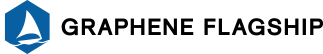
\includegraphics[height=0.5in]{title/logos/flagship}
\end{center}
\vfill

\noindent
\begin{tabular}{@{}p{0.2\textwidth}@{}p{0.8\textwidth}}
    \textit{Keywords:} & \ldots \\[\medskipamount]
    \textit{Printed by:} &  \\[\medskipamount]
    \textit{Front \& Back:} & Beautiful cover art that captures the entire content of this thesis in a single illustration.
\end{tabular}

\vspace{4\bigskipamount}

\noindent Copyright \textcopyright\ 2020 by F.E.~Schmidt

%% Uncomment the following lines if this dissertation is part of the Casimir PhD
%% Series, or a similar research school.
%\medskip
%\noindent Casimir PhD Series, Delft-Leiden 2015-01

\medskip
\noindent ISBN 000-00-0000-000-0

\medskip
\noindent An electronic version of this dissertation is available at \\
\url{http://repository.tudelft.nl/}.

\end{titlepage}


%%%%
%%%%%% The (optional) dedication can be used to thank someone or display a significant quotation.
%\dedication{
%	Für Katrin und Felicitas
%	\vskip 10\baselineskip
%	\textit{Remember, kids, the only difference between screwing around and science is writing it down.}
%	\vskip 0.5\baselineskip
%	Adam Savage, quoting Alex Jason in the 2012 MythBusters episode \textit{Titanic Survival}~\cite{savageOriginOnlyDifference2015}
%}
%\newchapstyle
%\tableofcontents
%\afterpage{\pagecolor{none}}
%%%
%%%
\chapter*{Summary}
\addcontentsline{toc}{chapter}{Summary}
\setheader{Summary}

{%\color{title}
Summary in English\ldots
}
\afterpage{\pagecolor{none}}

\chapter*{Samenvatting}
\addcontentsline{toc}{chapter}{Samenvatting}
\setheader{Samenvatting}

%% {\selectlanguage{dutch}


\afterpage{\pagecolor{none}}

\chapter*{Zusammenfassung}
\addcontentsline{toc}{chapter}{Zusammenfassung}
\setheader{Zusammenfassung}

%% {\selectlanguage{german}


\afterpage{\pagecolor{none}}

%%% Use Arabic numerals for the page numbers of the chapters.
\mainmatter

%%% Turn on thumb indices.
\thumbtrue

\newchapstyle
\chapter{Introduction}
\label{chap:intro}

%\epigraph[0pt]{
%    Failure is not an option.
%}{Actor Ed Harris, playing flight director Gene Kranz, in the 1995 film Apollo 13\cite{FailureNotOption2019}}

%\begin{abstract}
%Lorem ipsum dolor sit amet, consectetur adipisicing elit, sed do eiusmod tempor incididunt ut labore et dolore magna aliqua. Ut enim ad minim veniam, quis nostrud exercitation ullamco laboris nisi ut aliquip ex ea commodo consequat. Duis aute irure dolor in reprehenderit in voluptate velit esse cillum dolore eu fugiat nulla pariatur. Excepteur sint occaecat cupidatat non proident, sunt in culpa qui officia deserunt mollit anim id est laborum.
%\end{abstract}

%% Start the actual chapter on a new page.
\afterpage{\pagecolor{none}}\newpage

\section{Computing with semi- and superconducting circuits}

The invention of the metal oxide semiconductor field-effect transistor (MOSFET, cf. Fig.~\ref{fig:introcomputing}(a)) laid the ground for the information age, in large parts shaping the world to be what we know it as today.
%
Pushed by continuous advances in material sciences, solid state physics and electrical engineering, the MOSFET is now the building block of all commercial computers.
%
Owing largely to the success of scalability from integrated circuits, today's state-of-the-art microprocessors can host more than 39.54 billion transistors on a single chip, with physical dimensions down to a few tens of nanometers, cf. Fig.~\ref{fig:introcomputing}(b)~\cite{mujtabaAMDEPYCRome2019}.
%
With the increasing transistor density and shrinking physical dimensions came however the realization, that alternative computation architectures to the one based on semiconducting transistors might be needed to satisfy society's desire for computation power, as there might be a limit to how dense logic circuits could be packed with current technology.
%
The slowing of Moore's law, originally predicting the doubling of transistor chip density every two years~\cite{mooreCrammingMoreComponents2006}, is an important reminder of this challenge.


Already before the invention of the MOSFET, circuits on the basis of superconducting switches called \enquote{cryotrons} were envisioned as a competitive alternative to semiconducting computers~\cite{buckCryotronASuperconductiveComputer1956,brockWillNSAFinally}.
%
The discovery of Josephson junctions (JJs), weak links between two superconductors, depicted in Fig.~\ref{fig:introcomputing}(e), in 1962~\cite{josephsonPossibleNewEffects1962,andersonProbableObservationJosephson1963} spured additional interest due to the possibility of sensing extremely small magnetic fields, their low power consumption and high switching speeds~\cite{mcdonaldPicosecondApplicationsJosephson1980}.
%
In parallel to the development of MOSFETs, Josephson junctions were hence envisioned as building blocks for superconducting logic circuits, with IBM being one of the main drivers at the time~\cite{anackerJosephsonComputerTechnology1980a}.
%
In an attempt to combine the best of two worlds, the versatility of a high gain transistor, and the low dissipation of superconducting circuits, proposals were made in the 1980s to merge these two elements into the Josephson field effect transistor (JoFET), cf. Fig.~\ref{fig:introcomputing}(c)~\cite{clarkFeasibilityHybridJosephson1980,gallagherThreeterminalSuperconductingDevices1985}.


While IBM eventually ceased to research Josephson junction computation due to an apparent supremacy of semiconducting computers~\cite{robinsonIBMDropsSuperconducting1983}, research continued at public institutions and universities, in part driven by Richard Feynman's ideas of building quantum machines to run complex calculations much more efficiently than any classical, MOSFET-based, computer~\cite{feynmanSimulatingPhysicsComputers1982}.
%
The late twentieth century then saw the birth of first prototypes for a quantum computing architecture, and it was realized that Josephson junctions could form the basis of quantum bits~\cite{martinisQuantumJosephsonJunction2020}.
%
Since then, global tech companies like IBM, Google, Microsoft and Intel are all heavily invested in this architecture, each following a slightly different path~\cite{steffenQuantumComputingIBM2011,aruteQuantumSupremacyUsing2019,linnNewMicrosoftBreakthroughs2020,vandersypenQuantumComputingSemiconductor2019}.
%
Superconducting quantum processors based on Josephson junctions embedded in microwave (MW) circuits, as pursued by IBM and Google, have culminated in the milestone of \enquote{quantum supremacy}, i.e. the threshold at which a quantum processor can execute an algorithm that would be prohibitively costly in terms of computing time and money for a classical computer to perform~\cite{aruteQuantumSupremacyUsing2019}.
%
As a side note, we would like to point out that the usefulness of Google's supremacy experiment, while still an impressive experimental achievement, is challenged and criticized by the IBM team~\cite{QuantumSupremacy2019}.




Figure~\ref{fig:introcomputing}(f) shows an image of Google's \enquote{quantum supremacy} processor \textit{Sycamore}.
%
The building block of these processors are transmon qubits.
%
These consist of a coplanar capacitance in series with superconducting quantum interference devices (SQUIDs), formed by two Josephson junctions in a loop.
%
To tune the states of the transmons, magnetic flux is threaded through the SQUID loop, supplied via on-chip current bias lines in close proximity to the SQUIDs.
%
While coherence times of several hundreds of microseconds show great potential for future devices~\cite{placeNewMaterialPlatform2020}, standard transmons come with a few drawbacks:
%
Already the very first implementation of a two-qubit transmon processor showed that magnetic fields can lead to significant cross talk coupling qubits several centimeters apart from each other~\cite{dicarloDemonstrationTwoqubitAlgorithms2009}.
%
Additionally, since the chips need to be operated at temperatures only fractions of a Kelvin above absolute zero in order to protect their coherence from thermal excitations, the cooling power of the refrigerator must not be exceeded.
%
This can be problematic with high qubit numbers, since the Joule heating caused by the tuning current through all individual flux lines might exceed the cooling power.
%
As the number of physical qubits increases, so does the challenge of shielding individual qubits from each other's bias lines, and retaining enough cooling power as to not induce thermal effects.

In contrast, replacing SQUIDs with the long-abandoned JoFET might be beneficial:
%
Applying gate voltages instead of running a current through a wire does not lead to thermal dissipation, which removes the cooling power constraint.
%
Additionally, cross-talk can be significantly reduced due to the nature of electric fields in gate capacitors being strongly confined to a small volume around the gate voltage lead.
%
Finally, JoFETs have consistently performed well under application of in-plane magnetic fields.
%
While the latter are not strictly necessary in transmon qubits (rather to be avoided) flux noise is one of the limiting factors of SQUIDs, to which JoFET-based qubits would be insensitive~\cite{casparisSuperconductingGatemonQubit2018}.
%
Even more important, magnetic field-compatible JoFETs are one of the requirements of qubits based on the Majorana architecture, which could result in significantly more coherent qubits due to their intrinsic topological protection~\cite{hyartFluxcontrolledQuantumComputation2013}.


\begin{figure}[t]
	\centering
	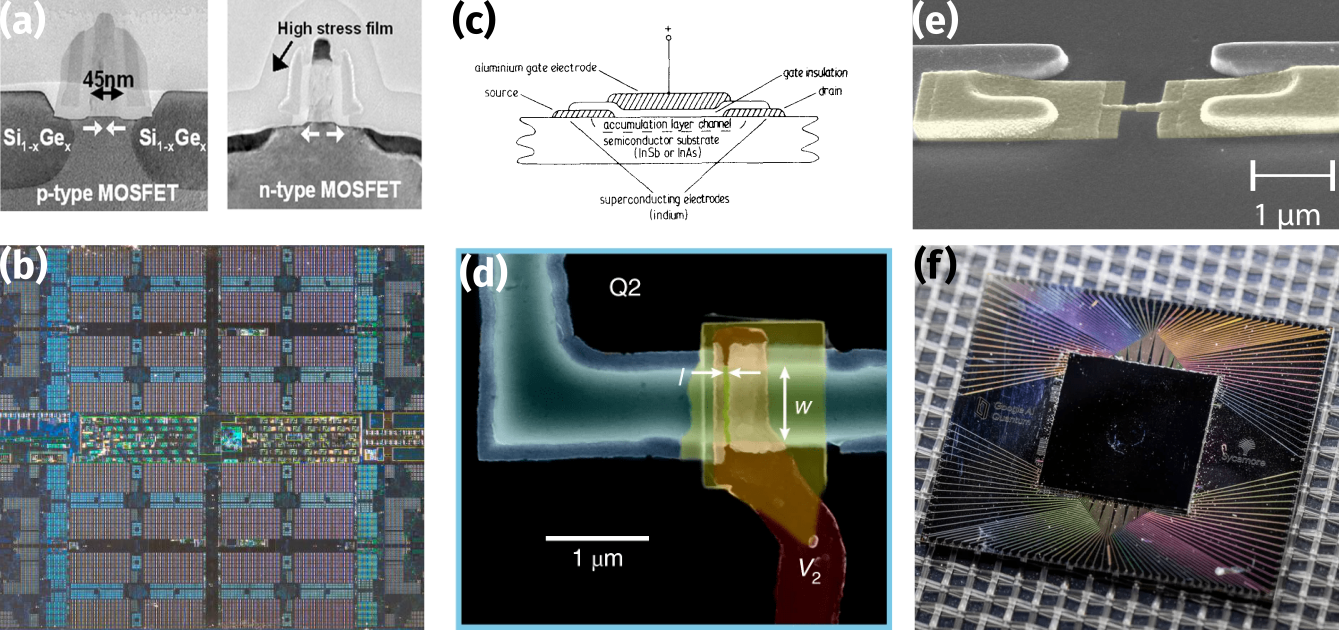
\includegraphics[width=\linewidth]{chapter-introduction/figs/intro_computing.svg.png}
	\caption{
		\textbf{Semi- and superconducting based computing devices.}
		%
		\textbf{(a)} Cross-sectional TEM image of \SI{45}{\nano\meter} node MOSFETs, the building block of semiconducting computers.
		%
		Figure adapted from~\cite{thompsonLogicNanotechnologyFeaturing2004}.
		%
		\textbf{(b)} Die shot of part of the I/O die of the microprocessor with currently highest number of transistors, in this case with \SI{14}{\nano\meter} node: The \textit{AMD Epyc Rome} with \num{8.34} billion transistors on the I/O die and \num{39.54} billion in total.
		%
		Figure adapted from \cite{fritzAMDRyzen36002019}.
		%
		\textbf{(c)} Sketch of the first envisioned JoFET as hybrid between semiconducting transistors and superconducting Josephson junctions.
		%
		Figure adapted from~\cite{clarkFeasibilityHybridJosephson1980}.
		%
		\textbf{(d)} SEM of a gatemon qubit, a potential building block for quantum computing on a hybrid super-semi approach.
		%
		Figure adapted from~\cite{casparisSuperconductingGatemonQubit2018}.
		%
		\textbf{(e)} SEM of an aluminum oxide Josephson junction, the workhorse of state-of-the-art superconducting microwave quantum  computing.
		%
		Figure adapted from~\cite{langfordExperimentallySimulatingDynamics2017}.
		%
		\textbf{(f)} Optical image of Google's \enquote{quantum supremacy} 53 qubit \textit{Sycamore} quantum processor.
		%
		Figure adapted from~\cite{shanklandTakeLookGoogle2020}. 
	}
	\label{fig:introcomputing}
\end{figure}

As of now, there has been only very little research in integrating JoFETs in superconducting quantum computing.
%
Recently, semiconductor nanowires and epitaxial 2DEGs were incorporated in transmon qubits, resulting in so-called \enquote{gatemons}, cf. Fig.~\ref{fig:introcomputing}(d)~\cite{delangeRealizationMicrowaveQuantum2015,larsenSemiconductorNanowireBasedSuperconductingQubit2015,casparisGatemonBenchmarkingTwoQubit2016a,casparisSuperconductingGatemonQubit2018,luthiEvolutionNanowireTransmon2018}.
%
While coherence times are not yet at the same level as for standard transmons, gatemons show great promise and have gained significant interest in the scientific community.
%
They not only provide a new way of controlling qubits~\cite{shimSemiconductorinspiredDesignPrinciples2016}, but also a path towards studying unconventional superconducting weak links at high frequencies~\cite{tahanGrapheneQubitMotivates2019}.





In this thesis, we initially set out to explore how JoFETs based on graphene Josephson junctions (gJJs) could perform in superconducting microwave circuits.
%
Since its discovery in 2004, graphene has shown versatile field effect applications and, already since very early on, gate-tunable superconductivity~\cite{novoselovElectricFieldEffect2004c,heerscheBipolarSupercurrentGraphene2007a}.
%
With improvements in contact engineering and reduced film disorder, induced superconductivity in gJJs has been a testbed for Andreev physics, phase coherent mechanisms, quantum phase transitions and the interplay of superconductivity and magnetism ~\cite{leeProximityCouplingSuperconductorgraphene2018a}.
%
Integrating gJJs in microwave circuits would thus be a first step towards the realization of gate-tunable superconducting microwave logic circuits.
%
In order to retain information about the device's DC properties, and to directly link them to the microwave performance, we chose to combine both DC and MW in one device.
%
To this end, we based our circuits on an architecture that allows simultaneous signal probing both with low and high frequencies: DC bias microwave cavities~\cite{bosmanBroadbandArchitectureGalvanically2015c}.
%
This not only allows for a detailed study of the junction's properties, but also enables applications based on current-biasing the sample.







\section{Josephson effects in SNS systems}

Josephson junctions are formed by a weak link between two superconducting electrodes, which must be sufficiently weak to sustain a phase difference $\delta=\phi_1-\phi_2$ between the phases of the two electrodes, $\phi_1$ and $\phi_2$, respectively.
%
Perhaps the simplest case of a JJ is a thin insulating tunnel barrier between two superconductors, the SIS JJ, cf. Fig.~\ref{fig:modelsnsdos}(a).
%
Here, Cooper pairs can tunnel from one superconductor through the barrier to the other side, while acquiring a phase $\delta$.
%
The current flowing across this type of junction is given by the junction's current phase relation (CPR), which for an SIS JJ reads
%
\begin{align}
I_\text{J}^\text{SIS}(\delta) &= I_\text{c}\sin\delta \ ,
\end{align}
%
with the critical current $I_\text{c}$.

The situation is different in the case in which the weak link consists of a normal metal between two superconducting banks, an SNS junction.
%
To support a supercurrent, the length of the normal metal must be smaller than the coherence length in the normal region, $L<\xi_\text{N}$, which in fact is much longer than the maximum thickness of the insulating barrier in the case of an SIS junction, where the thickness has to be smaller than the superconducting coherence length, $t\ll\xi_\text{S}$~\cite{caladoBallisticJosephsonJunctions2015d,benshalomQuantumOscillationsCritical2015}.
%
The process of Andreev reflection at the interface between superconductors and normal metals lays the basis for understanding how an SNS junction works~\cite{blonderTransitionMetallicTunneling1982c}.
%
The process is sketched in Fig.~\ref{fig:modelsnsdos}(b):
%
an electron impinging onto the super-normal interface from inside the normal region can only enter the superconductor in the form of a Cooper pair by being reflected as a hole with opposite spin and momentum.
%
Vice versa, a Cooper pair travelling towards the normal region will decay into an electron travelling forward, and annihilate a hole travelling backwards with spin opposite to that of the electron.
%
Inside the normal region, this will result in the formation of the so-called Andreev bound states (ABS) and a net current across the JJ.

\begin{figure}[t]
	\centering
	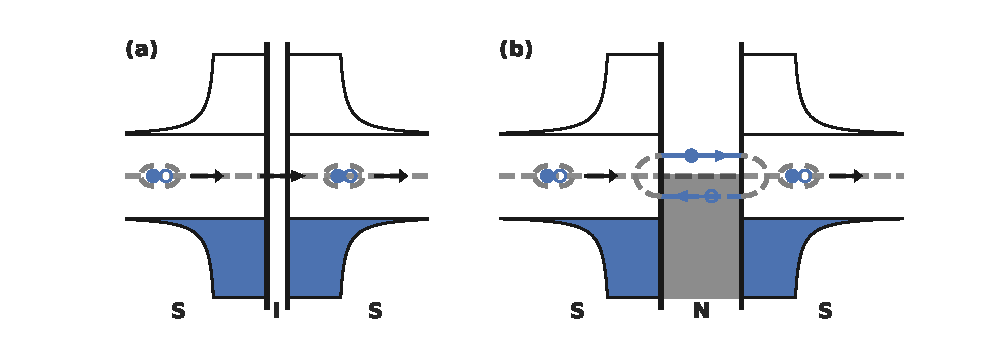
\includegraphics[width=\linewidth]{chapter-introduction/figs/model_SNS_DOS}
	\caption{
		\textbf{Cooper pair transport in SIS and SNS Josephson junctions.}
		%
		The density of states in a superconductor exhibits a gap of width $2\Delta$ in energy around the Fermi level $\epsilon_F$, with states below $\epsilon_F$ filled and states above unoccupied.
		%
		\textbf{(a)} In an SIS Josephson junction, Cooper pairs, consisting of an electron and hole with opposite spins and momentum, can tunnel through a thin insulating barrier separating two superconducting banks.
		%
		There are no states inside the insulating region.
		%
		\textbf{(b)} In an SNS Josephson junction, the normal region exhibits a DOS that is filled up to $\epsilon_F$.
		%
		Unpaired electrons can enter the superconductor by Andreev reflection as a hole with opposite momentum.
		%
		Conversely, Cooper pairs can enter the normal region by breaking into an electron and hole of opposite spin and momentum.
		%
		This way, Andreev bound states form within the normal region and a net current flows across the junction.
	}
	\label{fig:modelsnsdos}
\end{figure}


The current-phase relation in SNS junctions takes on a significantly different form than the sinusoidal one in SIS junctions:
%
For the simplest case of a one-dimensional SNS junction with perfect contact transparency $\tau_\text{c}=1$ at the SN interface, each Andreev bound state has a ground state energy
%
\begin{align}
E_{i}^{\rm ABS} = -\Delta\sqrt{1-T_i\sin^2 (\delta/2)}
\label{eq:ABS}
\end{align}
%
with the gap energy in the superconducting regions $\Delta$ and channel transparency $T_i$, where $T_i$ takes into account scattering inside the normal region~\cite{beenakkerUniversalLimitCriticalcurrent1991,titovJosephsonEffectBallistic2006b}.
%
Scattering at the SN interface, i.e. $\tau_\text{c}<1$, is not taken into account here in this simplified picture, as there is no closed analytical expression~\cite{blonderTransitionMetallicTunneling1982c}.
%
The energy of the excited ABS has opposite sign.
%
Summing over all channels in the junction, the total Josephson potential is given by
%
\begin{align}
U_\text{J}(\delta) = \Delta-\sum_i E_{i}^{\rm ABS} \approx E_\text{J} \frac{\delta^2}{2} - E_\text{J}\left( 1-\frac{3\sum T_i^2}{4\sum T_i} \right) \frac{\delta^4}{24} +\mathcal{O}(\delta^6)%\ , \\
%E_\text{J} &= \frac{\Delta}{4}\sum_i T_i \rightarrow \frac{\Delta}{4}N\tau
\end{align}
%
where we Taylor-expanded Eq.~\ref{eq:ABS}~\cite{kringhojAnharmonicitySuperconductingQubit2018}.
%
In the limit of low $T_i$, i.e. for an SIS junction, the energy would be given simply by $U_\text{J}^\text{SIS}(\delta)/E_\text{J}=1-\cos(\delta)\approx \delta^2/2-\delta^4/24$.
%
Compared to the SIS case, we therefore find that the Josephson energy is reduced by a fraction depending on the channel transparency which will become important for gatemon qubits, cf. Ref.~\cite{kringhojAnharmonicitySuperconductingQubit2018} and Chapter~\ref{chap:gJJ-CPR}.
%
We plot the ground and excited state energies of the ABS in Fig.~\ref{fig:modelsnsejic}(a).
%
With increasing channel transmission, $U_\text{J}$ exhibits stronger modulation and a closing band gap at $\delta=\pi$ with minimum separation $2\Delta\sqrt{1-\tau}$.

The corresponding relation between Josephson current and the respective phase drop across the one-dimensional SNS JJ is 
\begin{align}
I_\text{J}(\delta) = \frac{2e}{\hbar}\frac{\partial U_\text{J}}{\partial\delta} = \frac{e\Delta}{2\hbar}\sum_i\frac{T_i\sin(\delta)}{\sqrt{1-T_i\sin^2(\delta/2)}}
\end{align}
%
In addition, we can see that the JJ behaves as a strong nonlinear inductor, with inductance
%
\begin{align}
L_\text{J}(\delta) &= \frac{\hbar}{2e}\left( \frac{\partial I_\text{J}}{\partial\delta} \right)^{-1} = \left(\frac{\hbar}{2e}\right)^2\left(\frac{\partial^2U_\text{J}}{\partial\delta^2}\right)^{-1} \nonumber\\
&= \frac{4\hbar^2}{e^2\Delta}\sum_i \frac{\left(1-T_i\sin^2(\delta/2)\right)^{3/2}}{4T_i\cos(\delta)\left(1-T_i\sin^2(\delta/2)\right)+T_i^2\sin^2(\delta)} \ .
\end{align} 


Both quantities are depicted in Fig.~\ref{fig:modelsnsejic}(b,c).
%
We can conclude two things:
%
First, the larger the channel transmission, the stronger the forward skew of the current phase relation, defined as deviation of the CPR maximum from phase $\pi/2$, $S=2\delta_{\rm max}/\pi -1$, and corresponding deviation to the SIS case.
%
Second, while also strongly nonlinear, the Josephson inductance of SNS junctions is significantly reduced compared to the SIS case, $L_\text{J}^\text{SIS}(\delta)=\hbar/(2eI_\text{c}\cos\delta)$.
%
On the other hand, for junctions where $I_\text{c}$ remains constant, the increase in forward skew leads to a decrease in $\partial I_\text{J}/\partial\delta$, and hence an increase in $L_J$ around zero phase.
%
After an inflection point at $\delta\approx0.3\pi$, the SIS inductance is larger than the one at finite transmission, $L_\text{J}^\text{SIS}>L_\text{J}(\tau)$.
%
This is shown in Fig.~\ref{fig:modelsnsejic}(d,e).
%
Since exact knowledge of the Josephson inductance is critical for operating transmon qubits, these deviations need to be investigated for future applications. 

\begin{figure}[t]
	\centering
	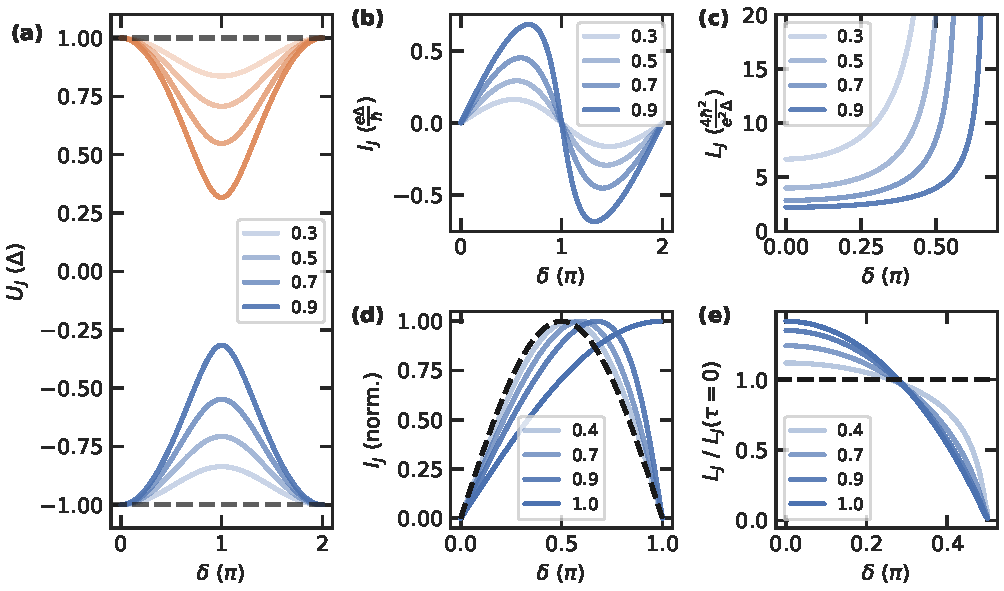
\includegraphics[width=\linewidth]{chapter-introduction/figs/model_SNS_EjIc_full}
	\caption{
		\textbf{Channel transmission and nonsinusoidality.}
		%
		\textbf{(a)} Josephson energy of the ground (blue) and excited (orange) Andreev bound state for varying channel transmission $\tau$ as a function of phase drop across the Josephson junction.
		%
		Increasing color intensity corresponds to increasing $\tau$.
		%
		Dashed line indicates the bulk gap $\pm\Delta$.
		%
		\textbf{(b)} Josephson current for varying $\tau$.
		%
		Increasing transmission increases both amplitude and forward skewing of the CPR.
		%
		\textbf{(c)} Josephson inductance as a function of phase. %normalized to the one at maximum $L_\text{J}$.
		%
		Due to the increased CPR slope for increasing $\tau$ around $\delta=0$, the Josephson inductance decreases significantly.
		%
		\textbf{(d)} Same as in \textbf{(b)}, but for constant critical current, hence only the forward skew increases.
		%
		Dashed line: CPR of an SIS junction.
		%
		\textbf{(e)} Josephson inductance as a function of transmission under the assumption of constant critical current as in \textbf{(d)}, compared to the case of an SIS junction (dashed line).
		%
		Around zero phase, $L_\text{J}$ increases with $\tau$, while for large phase bias, the inductance of an SIS JJ is in fact larger than the one of a junction with finite transmission.
	}
	\label{fig:modelsnsejic}
\end{figure}

For a realistic SNS junction such as the two-dimensional graphene devices measured in this thesis, there are a number of effects that lead to deviations of the above presented mechanisms.
%
The exact nature of the subgap density of states for example depends on size and geometry of the junction, as well as the contact transparency.
%
If the junction is sufficiently wide that the transport is no longer strictly one-dimensional, the ABS energy is reduced and moves closer to zero.
%
The same holds for the case of long compared to short junctions, cf. Fig.~\ref{fig:modelsubgap}:
%
This can be understood qualitatively by an effective energy $E_{\rm Th^*}=\hbar v_\text{F}/\Lambda<\Delta$ governing transport inside the junction, analogously to the Thouless energy~\cite{benshalomQuantumOscillationsCritical2015,schmidtBallisticGrapheneSuperconducting2018}, with an effective length scale $\Lambda=L/\tau$ and the Fermi velocity $v_\text{F}$.
%
In the case of a very wide junction, the transverse Thouless energy $E_{\rm Th^*}^\parallel=\hbar v_\text{F}/\Lambda_\parallel$ with $\Lambda_\parallel=W/\tau$ needs to be introduced.
%
The lower this energy, the longer the dwell time of ABS inside the normal region, hence their lower energy.
%
Finally, reduced contact transparency $\tau_\text{c}<1$ at the SN interface leads to the ABS detaching from the bulk gap at $\Delta$ even for zero phase difference~\cite{bretheauTunnellingSpectroscopyAndreev2017a}.


Figure~\ref{fig:modelsubgap} shows the calculated subgap density of states (DOS) for a exemplary graphene Josephson junction in the short and long regime, i.e. $L_\text{N}\ll\xi$ and $L_\text{N}>\xi$.
%
We find that for both cases the states with lowest energies are located at large parallel momentum $k_\parallel$, and that for the long junction, there are a number of subgap states below the bulk gap energy $\Delta$.
%
This significantly reduced gap can potentially absorb RF excitations, leading to dissipation and decoherence in microwave circuits.
%
Finally, graphene shows strong angle-dependent transport due to Klein-tunneling at interfaces, which collimates charge carrier transport perpendicular to interfaces at pn junctions, which can further modify the DOS~\cite{beenakkerColloquiumAndreevReflection2008}.

\begin{figure}[t]
	\centering
	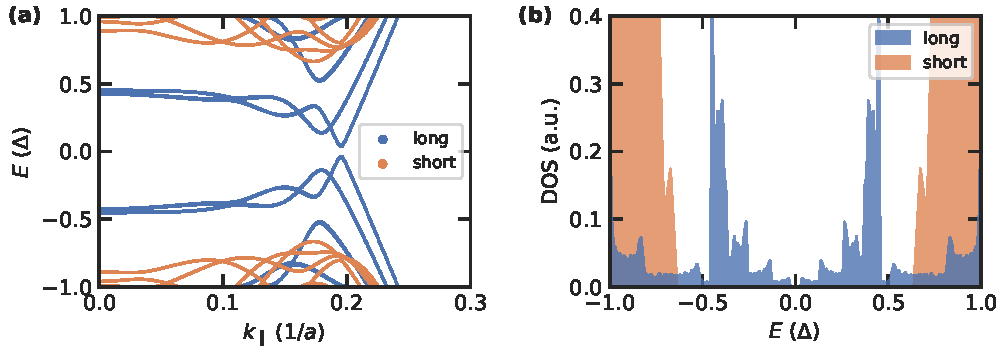
\includegraphics[width=\linewidth]{chapter-introduction/figs/kwant_modeling_181206_subgap_length_supp_Plot_subgap_dos}
	\caption{
		\textbf{Realistic subgap states of a 2D graphene Josephson junction.}
		%
		Tight-binding simulations of a graphene Josephson junction show strong dependence of the subgap state energies on momentum parallel to the SN interface \textbf{(a)}, with lowest lying energies at large $k_\parallel$.
		%
		While the short JJ (orange) shows an only slightly reduced minimum energy and DOS \textbf{(b)} compared to $\Delta$, long junctions (blue) exhibit heavily reduced energy gaps.
	}
	\label{fig:modelsubgap}
\end{figure}

In order to build reliable, reproducible circuits out of SNS junctions, it is thus vital to characterize them not only in the DC, but also in the microwave regime, as this is where the inductance will be measurable.
%
To this end, we placed our junctions in a circuit allowing for steady and high frequency signals to probe our device.
%
These DC bias microwave circuits are described in the following section.

\section{DC bias cavities for probing Josephson junctions}

\begin{figure}[t]
	\centering
	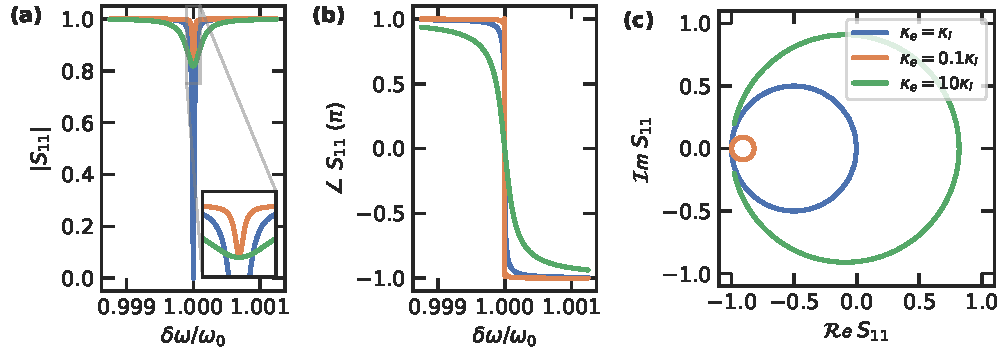
\includegraphics[width=\linewidth]{chapter-introduction/figs/model_DC_bias_cavity_coupling.pdf}
	\caption{
		\textbf{Effect of coupling ratio on the reflection coefficient of a DC bias cavity.}
		%
		Using Eq.~\ref{eq:intro-s11}, we can model the absolute value \textbf{(a)}, phase \textbf{(b)} and real and imaginary parts \textbf{(c)} of the reflection coefficient of a DC bias cavity.
		%
		Colors denote the various coupling types: blue: critically coupled $\kappa_\text{e}/\kappa_\text{i}=1$, orange: undercoupled $\kappa_\text{e}/\kappa_\text{i}=0.1$, green: overcoupled $\kappa_\text{e}/\kappa_\text{i}=10$.
		%
		Strongest signal modulation in $\abs{S_{11}}$ is achieved for critical coupling, while the other two cases have an identical minimum reflection coefficient.
	}
	\label{fig:s11}
\end{figure}


To probe the Josephson inductance, we make use of superconducting microwave resonators based on coplanar waveguides~\cite{gopplCoplanarWaveguideResonators2008,zmuidzinasSuperconductingMicroresonatorsPhysics2012}.
%
These have been used extensively in the field of particle detection and circuit (quantum) electrodynamics due to their intrinsic low loss originating from the fact that Cooper Pairs do not contribute any electrical resistance~\cite{dayBroadbandSuperconductingDetector2003a,blaisCavityQuantumElectrodynamics2004c,clerkHybridQuantumSystems2020,blaisQuantumInformationProcessing2020}.
%
For probing the device under test both in the low and high frequency range (DC to several $\SI{e9}{\hertz}$), our circuits need to sustain a stable resonance when biased with direct currents.

There is a variety of circuit architectures capable of this approach, such as using inductive coupling~\cite{vissersFrequencytunableSuperconductingResonators2015b}, direct leads at voltage nodes of a $\lambda/2$ resonator with matching length~\cite{chenIntroductionDcBias2011a,liApplyingDirectCurrent2013} or lumped-element split-cavities~\cite{mahashabdeFastTunableHigh2020}.
%
In contrast, we based our design on an architecture previously developed in our group: the shunt capacitor DC bias cavity~\cite{bosmanBroadbandArchitectureGalvanically2015c}.
%
This circuit has several advantages over the previously mentioned ones:
%
as no circuit symmetries need to be considered, the circuit layout is rather simple.
%
Because the shunt capacitor is placed at the input port to the device, no additional port needs to be used to probe or excite the device under test (DUT), which prevents additional leakage channels.
%
Finally, using a shunt capacitor provides a broadband signal port up to the self-resonance of the shunt capacitor, which is chosen to be well above the resonance frequency of the circuit.
%
The reflection coefficient of this circuit is given by
%
\begin{align}
S_{11}=-1+\frac{2\kappa_\text{e}}{\kappa_\text{e}+\kappa_\text{i}+2i\Delta}
\label{eq:intro-s11}
\end{align}
%
with the internal and external loss rates $\kappa_\text{i}$ and $\kappa_\text{e}$ and the detuning $\Delta=\omega-\omega_0$~\cite{bosmanBroadbandArchitectureGalvanically2015c}.
%
In Fig.~\ref{fig:s11} we plot the reflection coefficient for various fractions of $\eta =\kappa_\text{e}/\kappa_\text{i}$, to illustrate the effects of over-, under- and critical coupling ($\eta >1$, $\eta <1$ and $\eta =1$, respectively).
%
For the signal to be strongest in terms of $\abs{S_{11}}$, i.e. the absorption dip reaching zero, the shunt capacitor $C_\text{s}$ should be designed such that $\kappa_\text{e}=\kappa_\text{i}$, with the external loss rate approximately given by
%
\begin{align}
\kappa_\text{e} &= \frac{\omega_0}{Q_e} = \frac{2}{\pi\omega_0Z_0^2C_\text{s}^2}
\label{eq:intro-kappae}
\end{align}
%
with external quality factor $Q_e$ and transmission line impedance $Z_0$.
%
Due to stray inductance of the shunt capacitor, there is an upper limit to the maximum feasible $C_\text{s}$ we can use while keeping the self-resonance of the latter well above $\omega_0$.
%
In practice, this limits $Q_e$ to approximately \num{100e3}.
%
However, when placing a JJ at the end of the TL, the internal loss rate can rise significantly.
%
For this reason, we typically design our circuits such that they would be overcoupled in the case of a short to ground instead of a JJ, anticipating a rise in $\kappa_\text{i}$.


\begin{figure}[t]
	\centering
	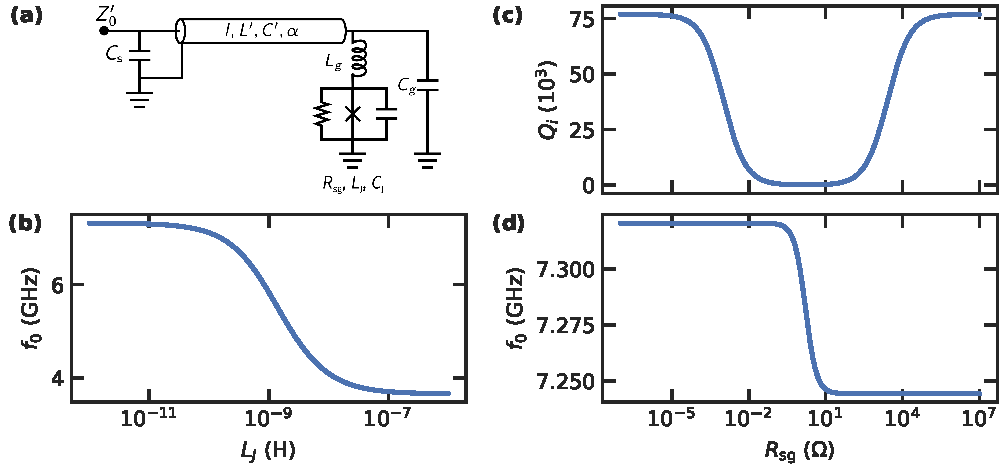
\includegraphics[width=\linewidth]{chapter-introduction/figs/model_DC_bias_cavity_params_RCSJ.pdf}
	\caption{
		\textbf{DC bias cavity shorted to ground by a parametrized top-gated graphene Josephson junction.}
		%
		\textbf{(a)} Fully parametrized circuit model.
		%
		The transmission line is described by length $l$, inductance and capacitance per unit length $L^\prime$ and $C^\prime$ and attenuation $\alpha$, and is coupled to an input impedance $Z_0^\prime$ via a shunt capacitance $C_\text{s}$.
		%
		The Josephson junction is modeled as a network of linear lead inductance $L_\text{g}$ together with an RCSJ model of subgap-resistance $R_\text{sg}$, junction capacitance $C_\text{J}$, nonlinear inductance $L_\text{J}$ and gate capacitance $C_\text{g}$.
		%
		In a realistic device (cf. Fig.~\ref{fig:fabgJJ}), the gate electrode has capacitances to both the lead $L_\text{g}$ and the transmission line.
		%
		For simplicity, we model $C_\text{g}$ as depicted here, and include additional capacitance in $C_\text{J}$.
		%
		For simulating the device in \textit{QUCS} however, we ignored $L_\text{g}$ and $C_\text{g}$ and used the following parameters (unless swept):
		%
		$Z_0=Z_0^\prime=\SI{50}{\ohm}$, $C_\text{s}=\SI{60}{\pico\farad}$, $l=\SI{6}{\milli\meter}/\sqrt{\epsilon_\text{r}}$ with the dielectric constant of silicon $\epsilon_\text{r}=11.7$, $\alpha=1.002$,  $L_\text{J}=\SI{36}{\pico\henry}$, $C_\text{J}=\SI{1}{\femto\farad}$, $R_\text{sg}=\SI{1}{\mega\ohm}$.
		%
		\textbf{(b)} Resonance frequency versus Josephson inductance with the other parameters fixed.
		%
		Depending on the junction impedance, the fundamental cavity mode changes from $\lambda/2$ (small $L_\text{J}$) to $\lambda/4$ (large $L_\text{J}$).
		%
		\textbf{(c,d)} Influence of subgap resistance on internal quality factor and resonance frequency.
		%
		Small $R_\text{sg}$ corresponds to a short, large $R_\text{sg}$ to an open to ground in parallel to $L_\text{J}$.
		%
		In both cases, the internal losses of the circuit are dominated by the transmission line attenuation.
		%
		For intermediate values of $R_\text{sg}$, significant resistive damping effectively suppresses the circuit response.
		%
		Panel \textbf{(d)} also illustrates the shift of $f_0$ when changing the boundary condition of the circuit, similar to the one due to $L_\text{J}$ in panel \textbf{(b)}.
	}
	\label{fig:TLmodel}
\end{figure}


When probing Josephson junctions with the DC bias cavity, we need to calibrate the parameters of the microwave circuit prior to extracting quantitative information on the high frequency properties of the added JJ.
%
Figure~\ref{fig:TLmodel}(a) depicts a schematic of the DC bias cavity with the relevant circuit parameters, including a second port to tune the DUT with a gate voltage.
%
We perform the calibration by measuring a combination of open and shorted reference device with the same sample geometry, except with an open or short to ground in place of the JJ.
%
Equipped with these values, we can proceed to study the influence JJ on the microwave circuit.
%
For modeling, we use the open-source tool \textit{Quite Universal Circuit Simulator} (QUCS~\cite{QucsProjectQuite}).




With an added Josephson junction with inductance $L_\text{J}$ shorting the TL to ground, and neglecting $R_\text{sg}$ and $C_{J}$, the shifted resonance frequency can be approximated by
%
\begin{align}
\omega_0^\prime = \omega_0\frac{L_\text{r}+L_\text{J}}{L_\text{r}+2L_\text{J}}
\label{eq:intro-omega0p}
\end{align}
%
where $L_\text{r}$ is the lumped TL resonator inductance including geometric and kinetic inductances, cf. Chapter~\ref{chap:gJJ-CPR} and Fig.~\ref{fig:TLmodel}(b).
%
A complete analytical model of an RSCJ model parametrizing the JJ can be used for calculating junction-induced losses in the form of a subgap resistance, cf. Chapter~\ref{chap:gJJ} and Fig.~\ref{fig:TLmodel}.
%
For very small $R_\text{sg}$, the Josephson inductance is effectively short-circuited, so both $Q_i$ and $f_0$ approach the limit of no JJ.
%
On the other hand, very large $R_\text{sg}$ implies an open circuit with no losses other than the ones in the TL resonator, again approaching $Q_i$ of the bare cavity and $f_0$ shifting the the value due to the added $L_\text{J}$.
%
Intermediate resistance values suppress the resonance entirely.
%
The shift in $f_0$ for large $R_\text{sg}$ shows the frequency shift induced by $L_\text{J}$.



\section{Outline}

In the following, we will show how DC bias cavities can be utilized to both extract information on the intrinsic microwave properties of a Josephson junction, and use the combination of cavity and junction to detect very small currents.

In chapter~\ref{chap:experiment}, we provide an overview on the experimental methods that we developed and used to enable the measurements presented later on.
%
We detail the exfoliation and fabrication of graphene and boron nitride, and the fabrication of gJJs and superconducting CPW resonators.
%
Additionally, a short introduction to the use of the superconducting alloy molybdenum-rhenium in Delft, together with a small study on its pros and cons, is supplied.
%
The chapter closes with a brief introduction to thermal noise and the fridge wiring used to suppress the former during measurements.

In chapter~\ref{chap:gJJ}, we present the first measurements of a graphene Josephson junction in the microwave regime.
%
Motivated by the potential use of graphene in superconducting quantum circuits, we studied the Josephson inductance by tracking the resonance frequency, and extracted the subgap resistance from the added circuit losses of the JJ.
%
Together with a detailed circuit characterization in both DC and the microwave regime, the results indicate that graphene Josephson junctions are indeed a feasible platform for circuit quantum electrodynamics.


In chapter~\ref{chap:gJJ-CPR}, we take a closer look at the underlying mechanism governing the Josephson inductance of graphene Josephson junctions, i.e. their current-phase relation.
%
Using the power and current bias dependence of our devices, we show that the CPR of diffusive and ballistic devices is forward-skewed, as is expected for these junctions.
%
We quantify the resulting correction of the Josephson energy potential, which is crucial for the use of gJJs in microwave quantum circuits.

We switch from pure fundamental studies of the junction's characteristics to a circuit application in chapter~\ref{chap:currentdetection}.
%
Instead of a graphene JoFET, we present a DC bias MW cavity coupled to an aluminum constriction Josephson junction, a so-called Dayem bridge~\cite{andersonRadioFrequencyEffectsSuperconducting1964}.
%
Making use of the responsivity of the circuit's resonance frequency to bias current, we detect low-frequency currents with a minimum sensitivity of \SI{8.9}{\pico\ampere\per\hertz\tothe{1/2}}, comparable to state-of-the-art devices.
%
With an analytical circuit model, we extrapolate orders of magnitude better values for improved device designs based on our circuit, which could eventually enable quantum limited current detection.


We close with a summary of all presented results and a possible way onwards in chapter~\ref{chap:conclusion}.
%
Appended to this thesis is a collection of additional DC data on graphene Josephson junctions and SQUIDs.
%
There, we investigate features in the IV curves that occur as a result of the junction interacting with its electromagnetic environment: Fiske and Shapiro steps.
%
The appendix additionally features tips and tricks for electron beam lithography, such as alignment and height measurements, specifications on the self-assembled low-pass and copper powder filters and miscellaneous source code.


%\clearpage
%\references{dissertation}


%\newchapstyle
\chapter{A ballistic graphene superconducting microwave circuit}
\label{chap:gJJ}

%% The following annotation is customary for chapter which have already been
%% published as a paper.
\blfootnote{\color{title}This chapter was published in \textit{Nature Communications} \textbf{9}, 4069 (2018) \cite{schmidtBallisticGrapheneSuperconducting2018a}.}

\begin{abstract}
Josephson junctions (JJ) are a fundamental component of microwave quantum circuits, such as tunable cavities, qubits and parametric amplifiers.
%
Recently developed encapsulated graphene JJs, with supercurrents extending over micron distance scales, have exciting potential applications as a new building block for quantum circuits. 
%  
Despite this, the microwave performance of this technology has not been explored.
%  
Here, we demonstrate a microwave circuit based on a ballistic graphene JJ embedded in a superconducting cavity.
%  
We directly observe a gate-tunable Josephson inductance through the resonance frequency of the device and, using a detailed RF model, we extract this inductance quantitatively. 
%
We also observe the microwave losses of the device, and translate this into sub-gap resistances of the junction at $\mu$eV energy scales, not accessible in DC measurements.
%
The microwave performance we observe here suggests that graphene Josephson junctions are a feasible platform for implementing coherent quantum circuits.
\end{abstract}

%% Start the actual chapter on a new page.
\newpage
\section{Introduction}

\noindent The development of ultra-high mobility graphene with induced superconductivity has led to ballistic transport of Cooper pairs over micron scale lengths, supercurrents that persist at large magnetic fields and devices with strongly non-sinusoidal current-phase relations \cite{caladoBallisticJosephsonJunctions2015d,benshalomQuantumOscillationsCritical2015,leeUltimatelyShortBallistic2015,novoselovRoadmapGraphene2012,walshGrapheneBasedJosephsonJunctionSinglePhoton2017}
While most measurements of such graphene Josephson junctions (gJJ) have been limited to the DC regime, Josephson junctions in general also play fundamental role in microwave circuits and devices such as qubits or quantum-limited amplifiers \cite{martinisCourse13Superconducting2004,castellanos-beltranDevelopmentJosephsonParametric2010}.

In these microwave applications, the Josephson junctions used are almost exclusively based on double-angle evaporated aluminum-aluminum oxide tunnel junctions (AlOx)\cite{dolanOffsetMasksLift1977a}, resulting in amorphous superconductor-insulator-superconductor (SIS) barriers.
Thus far, despite its robust and tunable superconductivity, graphene has not been implemented in this kind of microwave circuitry.
Apart from potentially addressing some of the design and stability issues with AlOx junctions \cite{zengDirectObservationThickness2015, zengAtomicStructureOxygen2016}, the use of gJJs in such circuits has the additional feature of allowing tunability of the junction properties through an electrostatic gate \cite{caladoBallisticJosephsonJunctions2015d,benshalomQuantumOscillationsCritical2015,leeUltimatelyShortBallistic2015,larsenSemiconductorNanowireBasedSuperconductingQubit2015,delangeRealizationMicrowaveQuantum2015}.
This feature can help address problems like on-chip heating and crosstalk in superconducting circuits where SQUIDs are used as tuning elements.\cite{schreierSuppressingChargeNoise2008a,sandbergTuningFieldMicrowave2008}.

Here, we present a superconducting microwave circuit based on a ballistic graphene JJ.
The design of our device is such that it also allows DC access to the junction, allowing us to directly compare the DC and RF response of our circuit.
While the gate-tunability enables us to directly tune the resonance frequency of the hybrid gJJ-resonator circuit, we also use the RF response to obtain additional information about the junction typically inaccessible through purely DC characterization.

\section{Results}

\begin{figure}[thb]
	\centering
	\includegraphics[width=\linewidth]{chapter-gJJ/figs/{fig1_final_cmyk.out}.pdf}
	\caption[]{
		\textbf{A gate tunable microwave cavity based on an encapsulated graphene Josephson junction. a,}
		Optical micrograph of the microwave cavity before placing the hBN/G/hBN stack.
		Bright areas are MoRe, dark areas are sapphire substrate.
		Grey area around the parallel plate capacitors is the \ce{Si3N4} shunt dielectric.
		Scale bar \SI{200}{\micro\meter}
		\textbf{b,} Optical micrograph of the gJJ. The cavity center line and the ground plane are connected through the gJJ and NbTiN leads.
		The gate line (right) extends over the entire junction.
		Scale bar \SI{40}{\micro\meter}
		\textbf{c,} Close-up of panel (b) with the graphene channel indicated.
		Dark areas are HSQ for gate insulation.
		Scale bar \SI{5}{\micro\meter}
		\textbf{d,} Sketch of the device circuit.
		The input signals are filtered and merged using a bias tee before being fed on to the feedline (see Methods section and Supplementary Fig. 1).
		\textbf{e,} Schematic cross-section of the gJJ with top-gate, not to scale.
		}
	\label{fig:figure1}
\end{figure}

\subsection{Circuit description}

The device presented here (Fig.\ref{fig:figure1}) consists of a galvanically accessible graphene Josephson junction embedded in a superconducting coplanar waveguide cavity.
The cavity superconductor is a molybdenum-rhenium (MoRe) alloy sputter-deposited on a sapphire substrate (Fig.\ref{fig:figure1}a).
The coupling to the external feedline is provided by a parallel plate shunt capacitor that acts as semi-transparent microwave mirror \cite{bosmanBroadbandArchitectureGalvanically2015c,singhMolybdenumrheniumAlloyBased2014}.
In contrast to series capacitors often used as mirrors, the use of shunt capacitors allows us to probe the circuit with steady-state voltages and currents, enabling DC characterization of the gJJ.
A circuit schematic of the device setup is depicted in Fig. \ref{fig:figure1}(d).
The gJJ is made from a graphene and hexagonal boron nitride (BN/G/BN) trilayer stack with self-aligned side contacts \cite{pizzoccheroHotPickupTechnique2016a,wangOneDimensionalElectricalContact2013b} using a sputtered superconducting niobium titanium nitride (NbTiN) alloy.
The stack is shaped into a junction of length $L=\SI{500}{nm}$ and width $W=\SI{5}{\micro m}$.
Here, $L$ and $W$ denote the distance between the superconducting contacts and lateral extension, respectively.
In order to tune the carrier density of the gJJ, a local DC gate electrode covers the junction and contact area.
Optical micrographs of the device are shown in Figs.\ref{fig:figure1}(b,c) and a schematic cross-section of the gJJ is shown in Fig.\ref{fig:figure1}(e).
Measurements of a similar second device can be found in Supplementary Figs. 10 and 11.

\subsection{DC characterization}

To compare our device with state-of-the-art gJJs, we first perform a purely DC characterization.
We sweep the current-bias ($I_\text{dc}$) and measure the voltage across the gJJ for different applied gate voltages ($V_\text{g}$).
The resulting differential resistance is plotted in Fig. \ref{fig:figure2}(a) and clearly shows a superconducting branch that is tunable through $V_\text{g}$.
The junction exhibits $I_\text{c}$ in the range of \SI{150}{nA} to \SI{7}{\micro A} for $\lvert V_\mathrm{G} \rvert<\SI{30}{V}$ with significantly lower $I_\text{c}$ for $V_\text{g}<0$ (p-doped regime) compared to $V_\text{g}>0$ (n-doped regime).
Comparing the bulk superconducting gap of our NbTiN leads with the junction Thouless energy, $\Delta/E_\text{th}\approx1.52>1$, our device is found to be in the intermediate to long junction regime (see Supplementary Note 7 and Supplementary Figs. 12, 15 and 16).

While in the non-superconducting state (current bias far above the junction critical current $I_\text{c}$), the graphene junction shows a narrow peak in its normal resistance associated with low disorder at the charge neutrality point (CNP, at $V_\text{g}\approx\SI{-2}{V}$, see Fig.\ref{fig:figure2}(b)), indicating high sample quality.
Some hysteresis in the switching and retrapping currents can also be observed in the measurement (see Supplementary Note 6 for discussion).
We furthermore observe oscillations in both the normal state resistance $R_\text{n}$ and the switching and retrapping currents as a function of gate voltage for p-doping of the channel.
We attribute these effects to the presence of PN junctions that form near the graphene-NbTiN contact.
Each of the two NbTiN leads n-dopes the graphene near the respective contact while the main sheet is p-doped by the gate.
The pair of PN junctions produce Fabry-P\'erot interference effects that give rise to the observed oscillations in $I_\text{c}$ and $R_\text{n}$.
The characteristics of these oscillations indicate that our junction is in the ballistic regime \cite{liangFabryPerotInterference2001,miaoPhaseCoherentTransportGraphene2007,youngQuantumInterferenceKlein2009,choMasslessMassiveParticleinabox2011,wuQuantumBehaviorGraphene2012,camposQuantumClassicalConfinement2012,rickhausBallisticInterferencesSuspended2013,benshalomQuantumOscillationsCritical2015,caladoBallisticJosephsonJunctions2015d,ametSupercurrentQuantumHall2016b,borzenetsBallisticGrapheneJosephson2016a,allenObservationElectronCoherence2017,zhuSupercurrentMultipleAndreev2018}.

\subsection{Microwave characterization}

\begin{figure}[thb]
	\centering
	\includegraphics[width=\linewidth]{chapter-gJJ/figs/{fig2_final_cmyk.out}.pdf}
	\caption[Observation of the Josephson inductance of a ballistic graphene superconducting junction]{\textbf{Observation of the Josephson inductance of a ballistic graphene superconducting junction. a,} Differential resistance across the gJJ for a wide gate voltage range.
		Dark blue denotes area of zero resistance.
		The device shows signatures of FP oscillations on the p-doped side.
		\textbf{b,} Normal state resistance of the gJJ versus gate voltage.
		\textbf{c,} Microwave spectroscopy of the device in the superconducting state versus gate voltage, plotted as the amplitude of the reflection coefficient $\lvert S_{11} \rvert$ after background subtraction.
		The graphene junction acts as a tunable inductor in the microwave circuit, resulting in a cavity frequency that is tuned with gate voltage.
		Inset: The resonance frequency oscillates in phase with the oscillations in \textbf{(a)} and \textbf{(b)}.}
	\label{fig:figure2}
\end{figure}

Having established the DC properties of our junction, we turn to the microwave response of the circuit.
Using a vector network analyser, we sweep a microwave tone in the 4 to \SI{8.5}{GHz} range and measure the reflection signal $S_{11}$ of the device for different applied gate voltages $\lvert V_\text{g} \rvert \leq \SI{30}{V}$.
The input powers and attenuation used correspond to an estimated intra-cavity photon number of at most 10-20 depending on operating frequency and linewidth.
Further tests were performed at lower powers (down to approximately 0.02 intra-cavity photons) with negligible changes to the cavity line shape and width.
More information on the measurement setup can be found in the Methods section and a detailed sketch in Supplementary Fig. 1.
Figure \ref{fig:figure2}(c) shows the resulting $\lvert S_{11}\rvert$.
A clear resonance dip associated to our device can be tracked as a function of applied gate.
The device exhibits a continuously tunable resonance frequency from \SI{7.1}{GHz} to \SI{8.2}{GHz} with higher frequencies at larger values of $|V_\text{g}|$.

\subsection{Josephson inductance of the gJJ}

\begin{figure}[thb]
	\centering
	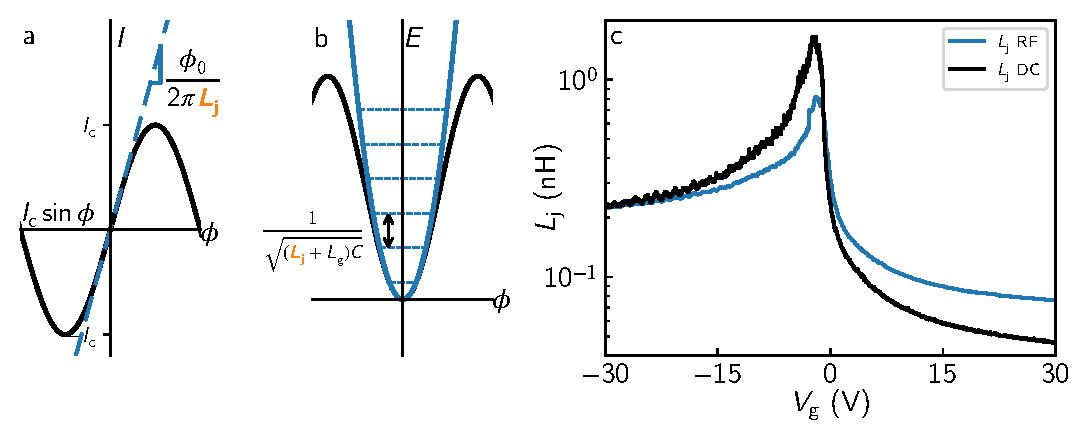
\includegraphics[width=\linewidth]{chapter-gJJ/figs/fig3_final}
	\caption[]{\textbf{Josephson inductance extracted from RF and DC measurements. a,}
		Schematic representation of $L_\text{j}$ and its relation to the CPR of a Josephson junction.
		$L_\text{j}$ can be understood as the slope of the current-phase relation around zero phase bias.
		\textbf{b,} Schematic representation of $L_\text{j}$ extraction from the cavity resonance frequency.
		The potential energy near $\phi = 0$ is harmonic, with the fundamental frequency given by the junction inductance $L_\text{j}$ and the cavity capacitance $C$ and inductance $L_\text{g}$ as $\omega = 1/\sqrt{(L_\text{j}+L_\text{g})C}$.
		\textbf{c,} Comparison of Josephson inductance $L_\text{j}$ extracted from DC measurements (black) and from the microwave measurements (blue).
		We attribute differences to deviations from a sinusoidal current phase relation (see main text for details).
		The error band from our fit of $L_\text{j}$ can be found in Supplementary Fig. 4.
	}
	\label{fig:figure3}
\end{figure}

The origin of the tunable circuit resonance frequency is the variable Josephson inductance of the graphene Josephson junction.
The microwave response of a JJ can be modelled for small currents using an inductor with its Josephson inductance given by:
\begin{equation}
L_\text{j} = \frac{\Phi_0}{2\pi} \left(\diff{I}{\phi}\right)^{-1}, \label{eq:Lj}
\end{equation}
where $\Phi_0$ is the flux quantum.
$L_\text{j}$ depends on the superconducting phase difference $\phi$ across the junction and on the derivative of the current-phase relation (CPR).
For small microwave excitations around zero phase ($\phi\simeq 0$) and assuming a sinusoidal CPR, $I=I_\text{c}\sin\phi$, this derivative is $_\text{d}I/_\text{d}\phi = I_\text{c}$.
This leads to an inductance $L_\text{j} = L_{\text{j}0} \equiv \frac{\Phi_0}{2\pi I_\text{c}}$ which can be tuned by changing the critical current of the junction.
In the device presented here, this junction inductance is connected at the end of the cavity.
When this inductance is tuned, it changes the boundary conditions for the cavity modes and hence tunes the device resonance frequency.
The effect can be illustrated by taking two extreme values of $L_\text{j}$ (see Supplementary Fig. 3):
If $L_\text{j}\rightarrow 0$ (i.e. $I_\text{c}\rightarrow\infty$), the cavity boundary conditions are such that it is a $\lambda/2$ resonator with voltage nodes at both ends.
If, on the other hand $L_\text{j}\rightarrow \infty$ ($I_\text{c}\rightarrow 0$), the cavity will transition into a $\lambda/4$ resonator with opposite boundary conditions at each end (a voltage node at the shunt capacitor and a current node at the junction end).
This leads to a fundamental mode frequency of about half that of the previous case.
Any intermediate inductance value lies between these two extremes.
Due to the inverse relationship between $I_\text{c}$ and $L_\text{j}$, the resonance frequency changes very quickly in certain gate voltage regions, having a tuning rate of up to $\mathrm{d}f_0/\mathrm{d}V_\text{g}=\SI{1.8}{GHz.V^{-1}}$ at $V_\text{g}=\SI{-0.54}{V}$.
This slope could potentially be further increased by increasing the gate lever arm, for example by choosing a thinner gate dielectric.
We again note that the resonance frequency does not saturate within the measured range although the tuning rate at $\vert V_\text{g} \rvert=\SI{30}{V}$ is much lower.
Additionally, by comparing Figs. \ref{fig:figure2}(a) and \ref{fig:figure2}(c), we can observe features in the RF measurements that are also present in the DC response.
In particular, the Fabry-P\'erot (FP) oscillations of $I_\text{c}$ and $R_\text{n}$ seen in the DC measurements result in a modulation of $L_\text{j}$, producing corresponding oscillations in the cavity frequency.
By analysing the oscillation period in reciprocal space, we extract a FP cavity length of $L_\text{c}\approx \SI{390}{nm}$ (see Supplementary Figs. 13 and 14).
We can thus take $L_\text{c}$ as a lower bound for the free momentum scattering and the phase coherence lengths, i.e. $l_\text{mfp},\xi>L_\text{c}$.

Further analysis of the data presented in Fig.\ref{fig:figure2}c can be used to perform a more quantitative analysis of the Josephson inductance of the gJJ as a function of gate voltage.
As illustrated in Fig. \ref{fig:figure3}(a) and equation (\ref{eq:Lj}), the Josephson inductance $L_\text{j}$ is defined according to the slope of the CPR near $\phi=0$ and sets the Josephson energy scale.
For a given assumed CPR, the inductance can be deduced from a DC measurement of the junction $I_\text{c}$.
When measuring the RF response of our device, the current in the junction oscillates with a very low amplitude around $\phi=0$.
This directly probes the CPR slope and the Josephson inductance at zero phase bias.
This inductance $L_\text{j}$ combined with the cavity inductance $L_\text{g}$ and capacitance $C$ determine the resonance frequency (Fig. \ref{fig:figure3}(b)).
An accurate calibration of the cavity parameters then allows us to extract $L_\text{j}$ from our measured resonance frequency without assuming any specific CPR.

To accurately obtain $L_\text{j}$ from our measurements, we calibrate the parameters of our RF model of the device using simulations and independent measurements, including effects of the kinetic inductance of the superconductor, the capacitance and inductance of the leads connecting the junction to the cavity, and the coupling to the external measurement circuit (see Supplementary Notes 1 and 2, Supplementary Fig. 2 and Supplementary Table 1) leaving only the junction characteristics as the remaining fit parameters.
By fitting the microwave response of the circuit, we obtain the resonance frequency as well as internal and external Q-factors voltage.
Using the model, we then translate this into an extracted inductance $L_\text{j}$ of the junction for each gate voltage.

Figure \ref{fig:figure3}c shows the resulting $L_\text{j}$ obtained from the dataset in Fig. \ref{fig:figure2}c compared to that obtained by assuming a sinusoidal CPR together with the DC switching currents from Fig. \ref{fig:figure2}a.
At low negative gate voltages we find excellent agreement between the DC and RF models.
As the gate voltage approaches the CNP, we observe clear differences, as the DC value of $L_\text{j}$ from a sinusoidal CPR overestimates the inductance obtained from the RF measurements.
For positive gate voltages, on the other hand, the DC value lies well below the one from our microwave measurements.

To understand the implications of these results, we start first with the p-doped regime. 
Since the gJJ is intermediate to long junction regime  and has low contact transparency at high p-doping due to PN junctions at the contacts, it is expected to have a sinusoidal CPR.
In this case, the DC values of $I_\text{c}$ should correctly predict Josephson inductance.
The clear agreement between the RF and DC values for $L_\text{j}$ in this regime is remarkable, and suggests that we have an accurate RF model of the circuit that can be used to extract direct information about the nature of our junction.
For high n-doping, the DC measurement yields much lower values of $L_\text{j}$ than the ones obtained from our RF measurements.
This is in agreement with the fact that high transparency and doping has been observed to produce forward skewing in gJJ CPR \cite{nandaCurrentPhaseRelationBallistic2017} which leads to an underestimation of $L_\text{j}$ if a sinusoidal CPR is used in the DC calculation.
On the other hand, the origin of the mismatch for $V_\text{g}$ around the CNP is unclear.
Although noise in the bias current can cause DC measurements to overestimate $L_\text{j}$, the noise present in our setup cannot account for this deviation.
Alternatively, using the same logic as in the high n-doping case, this deviation could be accounted for with a backward skewed CPR.
However, this is contrary to what has been reported in previous measurements on graphene \cite{englishObservationNonsinusoidalCurrentphase2016}.

\subsection{Microwave losses in the gJJ}

\begin{figure}[thb]
	\centering
	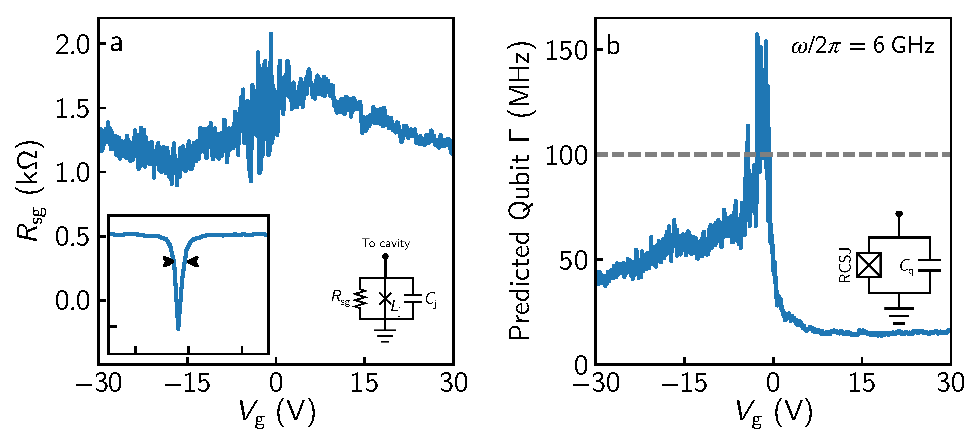
\includegraphics[width=\linewidth]{chapter-gJJ/figs/fig4_final}
	\caption[]{\textbf{Subgap resistance from microwave cavity measurements.} 
		\textbf{a,}
		Extracted sub-gap resistance at as a function of gate voltage.
		The values are calculated by calibrating the cavity properties and using the junction model shown connected to the transmission line cavity to fit the observed cavity response.
		Inset shows the cavity response at $V_\text{g}=\SI{30}{V}$.
		The horizontal and vertical axis divisions are \SI{10}{MHz} and \SI{10}{dB} respectively.
		\textbf{b,}
		Predicted linewidth for a graphene transmon qubit, obtained by taking the RCSJ parameters as a function of gate and adding a capacitance $C_\text{q}$ such that the final operating frequency remains $\omega/2\pi = \left(2\pi\sqrt{(L_\text{j}(C_\text{j}+C_\text{q}))}\right)^{-1} = \SI{6}{GHz}$.
		We assume the internal junction losses dominate the total linewidth.
		The horizontal line represents the anharmonicity of a typical SIS transmon $E_\text{c}/h=\SI{100}{MHz}$.
		In regions where the blue line falls under the dashed line, a gJJ transmon would be capable of operating as a qubit.
		The error bands for both panels can be found in Supplementary Fig. 5.
	}
	\label{fig:figure4}
\end{figure}

While tracking the resonance frequency as a function of gate voltage enables us to extract the Josephson inductance, the resonance linewidth provides information about the microwave losses of the gJJ.
The resonance linewidth is also observed to depend on the gate voltage, with minimum values of $\Gamma\sim\SI{2}{MHz}$ at high $|V_\text{g}|$ and a maximum of \SI{80}{MHz} near the CNP.
We use measurements of an identical circuit without the graphene junction as a benchmark to calibrate the internal and external cavity linewidths.
Using this benchmark together with a model for the junction losses, we find the correct combination of junction parameters that provide the observed frequency and cavity linewidth.
This allows us to quantify the amount of microwave losses attributable to the junction.

We describe the junction using the Resistively Capacitively Shunted Junction (RCSJ) model where the losses are parametrized by a dissipative element $R_\text{j}$.
For voltages larger than the superconducting gap $\Delta$ the effective resistance $R_\text{j} = R_\text{n}$ is that of normal state graphene.
The RF currents applied in our experiment, however, are well below $I_\text{c}$, and the associated voltages are also well below the bulk superconducting gap.
In this regime, the correct shunt resistance for the RCSJ model is not the normal state resistance $R_\text{n}$ but instead given by the zero-bias sub-gap resistance $R_\text{j} = R_\text{sg}$.
This quantity, which ultimately determines the junction performance in microwave circuits, has not been observed before in graphene as it is only accessible through sub-microvolt excitations, which are difficult to achieve in DC measurements.

As shown in Fig. \ref{fig:figure4}a, the zero-bias sub-gap resistance is of the order of \SIrange{1}{2}{\kilo\ohm} and remains relatively flat on the range of applied gate voltages.
We find that the ratio $R_\text{sg}/R_\text{n}$ has values around 10-40, depending on gate voltage, with higher values in the n-doped regime.
This ratio is often taken as figure of merit in SIS literature, as lower values of $R_\text{sg}$ are detrimental to most applications since they imply higher leakage currents in DC and more dissipation in RF.

While $R_\text{sg}$ of our device is lower than what would be implied by the coherence times in qubits based on low-critical-current oxide SIS junctions \cite{paikObservationHighCoherence2011g}, the $R_\text{sg}/R_\text{n}$ ratio is comparable to typical values from DC measurements of SIS devices with larger critical currents \cite{iosadCharacterizationFabricationProcess2002b,tolpygoSubgapLeakageHboxNb2013}.

The finite sub-gap resistance in superconductor-semiconductor devices is not fully understood, but is thought to originate from imperfect contact transparency, charge disorder and anti-proximity effects \cite{liuPhenomenologySoftGap2017a,bretheauTunnellingSpectroscopyAndreev2017a}.
While state-of-the-art SNS devices based on epitaxial semiconductors only recently exhibited hard induced gaps \cite{changHardGapEpitaxial2015,kjaergaardQuantizedConductanceDoubling2016}, there are to our knowledge no reports of this on graphene devices, suggesting an interesting direction for future research.
Another effect leading to finite sub-gap conductance is the size of our device, which is much larger and wider than usually employed junctions in microwave circuits.
Depending on the ratio of $\Delta$ to the effective round-trip time of sub-gap states across the junction, the Thouless energy $E_\text{th}$, the sub-gap density of states can be non-negligible.

From previous reports\cite{rosdahlAndreevRectifierNonlocal2018}, and from simulations of our channel (see Supplementary Note 7 and Supplementary Fig. 12), it is expected that there are a number of low-lying sub-gap states that could limit the value of $R_\text{sg}$.
This suggests that the losses could be reduced ($R_\text{sg}$ increased) by moving towards the short junction regime in which the energies of these states are increased and hence a harder gap forms.
To maintain the same inductance $L_\text{j}$, the junction would also have to be made narrower to compensate for the higher critical currents associated with a shorter junction.
This would presumably further enhance $R_\text{sg}$ since low-lying sub-gap states typically originate from states with high transverse momentum.
Given the fact that the geometry and aspect ratio of our junction is not at the limit of state-of-the-art fabrication capabilities, reducing the size is a promising step to reduce the losses in future gJJ based devices.

We finally analyse the potential performance of our device for circuit quantum electrodynamics (cQED) applications.
We consider the performance of a hypothetical transmon qubit \cite{kochChargeinsensitiveQubitDesign2007b} using the inductance of our gJJ operating at $\omega/2\pi=\SI{6}{GHz}$.
Assuming that the qubit losses are dominated by $R_\text{sg}$, the quality factor of such a device is given by $R_\text{sg}/(\omega L_\text{j})$ which in our case is of the order of a few hundred, a reasonable value considering further optimization steps can be taken.
In order to qualify as a qubit, the resonator linewidth should be smaller the transmon anharmonicity, given by the charging energy $E_\text{c}$.
In Fig. \ref{fig:figure4}b, we compare the predicted gJJ transmon linewidth $\Gamma$ with a typical value for the anhamonicity of SIS transmon qubits, $E_\text{c}/h = \SI{100}{MHz}$.
For a wide range of gate voltages, we find that the predicted linewidth is smaller than the anhamonicity, $\Gamma < E_\text{c}/h$, a promising sign for qubit applications of the technology.
We note, however, that the critical currents of this junction would be too high at large gate voltages (i.e. our Josephson inductances are too low), requiring a capacitor that would be too large to satisfy the condition $E_\text{c}/h \geq \SI{100}{MHz}$ and a resonant frequency of \SI{6}{GHz}.
To reduce the critical current (and increase the Josephson inductance), a narrower junction could be used, which could also increase the subgap resistance, further improving the performance.
A more in-depth discussion on this point is included in Supplementary Notes 3-5 and Supplementary Figs. 6-8.
We believe that implementing a graphene transmon qubit with good coherence times is feasible for future devices.
We also note that while the ballistic nature of the junction is not crucial for its operation in the microwave circuit, the lack of electronic scattering in the channel offers a nice platform to better understand the loss channels in comparison to highly disordered systems, with a potential to use this knowledge in the future to optimize devices. 

\section{Discussion}

In summary, we have measured a ballistic encapsulated graphene Josephson junction embedded in a galvanically accessible microwave cavity.
The application of an electrostatic gate voltage allows tuning of the junction critical current as well as the cavity resonance frequency through the Josephson inductance $L_\text{j}$.
While the DC response of the junction is broadly in line with previous work \cite{caladoBallisticJosephsonJunctions2015d,benshalomQuantumOscillationsCritical2015,leeUltimatelyShortBallistic2015}, the RF measurement of the cavity-junction system provides additional information on $L_\text{j}$ and microwave losses in this type of junction.
A comparison of the DC and RF derived values of $L_\text{j}$ reveal deviations from sinusoidal current phase relations, including suggestions of features not previously observed, demonstrating that microwave probes can reveal new information about the junction physics. 
From the microwave losses of the resonance, we have extracted the junction sub-gap resistance and predicted that, with some optimization, it should be possible to make a coherent qubit based on a gJJ.
From the physics of the proximity junctions, we have suggested a route towards improving the coherence potentially towards the current state-of-the-art, enabling a new generation of gate-tunable quantum circuit technology. 


\section{Methods}
\subsection{Fabrication of the microwave circuit}
We closely follow a recipe published earlier \cite{bosmanBroadbandArchitectureGalvanically2015c,singhMolybdenumrheniumAlloyBased2014}.
In short, a \SI{50}{nm} film of MoRe is first sputtered onto a 2" sapphire wafer (\SI{430}{\micro m}, c-plane, SSP from \textit{University Wafers}).
The coplanar waveguide (CPW) resonator is defined using positive e-beam lithography and dry-etching with an $\mathrm{SF_6 + He}$ plasma.
We subsequently deposit \SI{60}{nm} of \ce{Si3N4} for the shunt dielectric using PECVD and pattern this layer with a negative e-beam step and a $\mathrm{CHF_3 + O2}$ plasma.
The top plate of the shunts consists of a \SI{100}{nm} layer of MoRe which is deposited using positive e-beam lithography and lift-off.
An additional shunt capacitor, identical to the one on the main input, is built on the gate line.
This will filter RF noise on the gate line and suppress microwave losses through this lead.
Finally, we dice the wafer into $\SI{10}{mm}\times\SI{10}{mm}$ pieces, onto which the BN/G/BN stacks can be deposited.

\subsection{Fabrication of the gJJ}
We exfoliate graphene and BN from thick crystals (HOPG from \textit{HQ Graphene} and BN from \textit{NIMS}\cite{taniguchiSynthesisHighpurityBoron2007}) onto cleaned Si/$\mathrm{SiO_2}$ pieces using wafer adhesive tape.
After identifying suitable flakes with an optical microscope, we build a BN/G/BN heterostructure using a PPC/PDMS stamp on a glass slide \cite{pizzoccheroHotPickupTechnique2016a,wangOneDimensionalElectricalContact2013b}.
The assembled stack is then transferred onto the chip with the finished microwave cavity.
Using an etch-fill technique ($\ce{CHF3} + \ce{O2}$ plasma and NbTiN sputtering), we contact the center line of the CPW to the graphene flake on one side, and short the other side to the ground plane.
Clean interfaces between the NbTiN junction leads and the MoRe resonator body are ensured by maximizing the overlap area of the two materials and immediate sputtering of the contact metal after etch-exposing the graphene edge.
The resistance measured from the resonator center line to ground is therefore due entirely to the gJJ.
After shaping the device ($\ce{CHF3} + \ce{O2}$ plasma), we cover it with two layers of HSQ \cite{nandaCurrentPhaseRelationBallistic2017} and add the top-gate with a final lift-off step.

\subsection{Measurement setup}\label{sec:setup}
\noindent A sketch of the complete measurement setup is given in Supplementary Fig. 1.
The chip is glued and wire-bonded to a printed circuit board, that is in turn enclosed by a copper box for radiation shielding and subsequently mounted to the mK plate of our dry dilution refrigerator.
All measurements are performed at the base temperature of \SI{15}{mK}.
Using a bias-tee, we connect both the RF and DC lines to the signal port of the device while a voltage source is connected to the gate line.

We perform the microwave spectroscopy with a Vector Network Analyser (Keysight PNA N5221A).
The input line is attenuated by \SI{53}{dB} through the cryogenic stages, and \SI{30}{dB} room temperature attenuators.
Adding to these numbers an estimate for our cable and component losses results in a total attenuation on our input line of approximately \SI{92}{dB}.
The sample is excited with \SI{-30}{dBm}, so less than \SI{-122}{dBm} should arrive at the cavity.
This corresponds to an estimated intra-cavity photon number of at most 10-20 depending on operating frequency and linewidth (see Supplementary Fig. 9).
Test were run at $V_\text{g} = \SI{30}{V}$ for powers down to \SI{-152}{dBm}, or approximately 0.02 photons, with negligible changes to the cavity line shape.
Other gate voltages are expected to have even lower photon populations for with the same setup due to the lower internal cavity Q-factor.
The reflected microwave signal is split off from the exciting tone via a directional coupler, a DC block, two isolators and a high-pass filter to reject any low-frequency noise coupling to the line.
The signal is furthermore amplified by a \SI{40}{dB} \textit{Low-Noise Factory} amplifier on the \SI{3}{K} plate, and two room-temperature \textit{Miteqs}, each about \SI{31}{dB}, leading to a total amplification of \SI{102}{dB}.
During all RF measurements, the bias current is set to zero.

The DC lines consist of looms with twelve twisted wire pairs, of which four single wires are used in the measurements presented here.
The lines are filtered with $\pi$-filters inside the in-house built measurement rack at room-temperature, and two-stage RC and copper-powder filters, thermally anchored to the mK plate.
To reduce the maximum possible current on the gate line, a \SI{100}{k\ohm} resistor is added at room-temperature.
For the DC measurements presented, we turn the output power of the VNA off and current-bias the gJJ, while measuring the voltage drop across the device with respect to a cold ground on the mK plate.

\subsection{Data visualization}
To remove gate-voltage-independent features such as cable resonances, we subtracted the mean of each line for constant frequency with outlier rejection (\SI{40}{\percent} low, \SI{40}{\percent} high) from the original data, resulting in Fig. \ref{fig:figure2}(c).
All figures representing data are plotted using \textit{matplotlib} v2 \cite{hunterMatplotlib2DGraphics2007}.

\subsection{Data Availability}
All raw and processed data as well as supporting code for processing and figure generation is available in Zenodo with the identifiers \verb|10.5281/zenodo.1296129|~\cite{schmidtDataCodeBallistic2018} and \verb|10.5281/zenodo.1408933|~\cite{jenkinsMeasurementAnalysisScripts2018}.

%%%%%%%%%%%%%%%%%%%%%%%%%%%%%%%%%%%
% Insert main.bbl contents here

%\input{main.bbl}


%%%%%%%%%%%%%%%%%%%%%%%%%%%%%%%%%%%
% Insert SM.tex contents here

\clearpage
\pagebreak
%\widetext

%\setcounter{equation}{0}
%\setcounter{figure}{0}
%\setcounter{table}{0}
%\setcounter{page}{1}
%\setcounter{section}{0}

%\renewcommand{\thepage}{S\arabic{page}}
%\renewcommand{\thesection}{S\Roman{section}}
%\renewcommand{\thetable}{S\Roman{table}}
%\renewcommand{\thefigure}{S\arabic{figure}}
%\renewcommand{\theequation}{S\arabic{equation}}
%\renewcommand{\bibnumfmt}[1]{[S#1]}
%\renewcommand{\citenumfont}[1]{S#1}

\begin{figure*}[]
	{\centering
		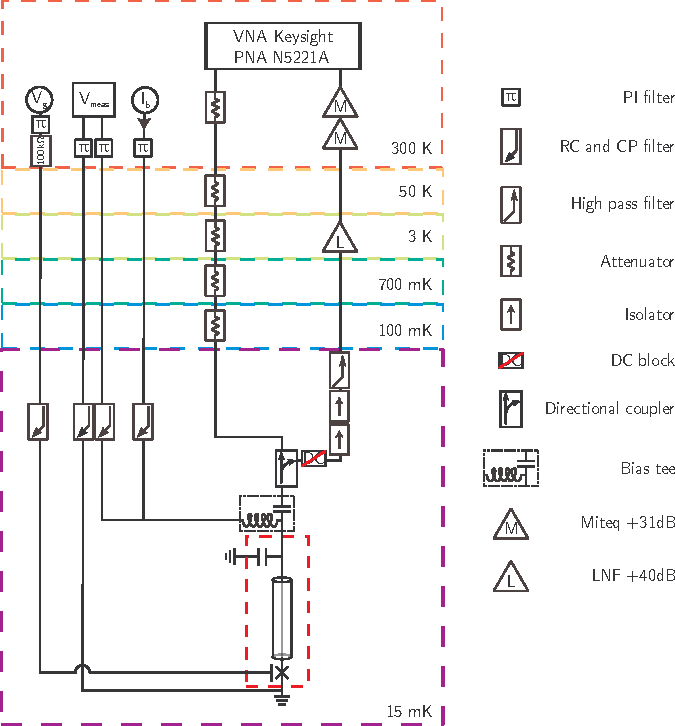
\includegraphics[width=\linewidth]{chapter-gJJ/figs/full_setup_cmyk}}
	\caption{{\bf Sketched measurement setup.}
		Dashed red box at the bottom marks device outline.
	}
	\label{fig:setup_full}
\end{figure*}

\clearpage
\section{Supplementary Material: A ballistic graphene superconducting microwave circuit}

%\vspace{1em}

%\makeatletter
%\renewcommand*{\fnum@figure}{{\normalfont Supplementary Figure~\thefigure}}
%\renewcommand*{\fnum@table}{{\normalfont Supplementary Table~\thetable}}
%% \renewcommand*{\@caption@fignum@sep}{\textbf{ : }}
%\makeatother
%\renewcommand{\thesection}{Supplementary Note \arabic{section}}
%\renewcommand{\bibsection}{\subsection*{SUPPLEMENTARY REFERENCES}}
%\setcounter{section}{0}
%\setcounter{figure}{0}

\subsection{Fitting routine for extracting the resonance frequency}\label{sec:fitting}
\noindent The microwave response function of a capacitively shunted resonator in reflection geometry is given by \cite{pozar_microwave_2012}
\begin{eqnarray}
\Gamma(\omega) = \frac{\kappa_\mathrm{ext}-\kappa_\mathrm{int}-2i\Delta\omega}{\kappa_\mathrm{ext}+\kappa_\mathrm{int}+2i\Delta\omega},
\end{eqnarray}
where $\kappa_\mathrm{ext,int}=\omega_0/Q_\mathrm{ext,int}$ are the internal and external loss rates and $Q_\mathrm{ext,int}$ are the respective quality factors.
$\Delta\omega=\omega-\omega_0$ is the frequency detuning from the resonance frequency $\omega_0$.

The measured reflection coefficient must also include the effect of the connecting wires and devices between the network analyser and the device under test.
The reflection coefficient is accordingly modified to incorporate this background:
\begin{eqnarray}
S_{11} = B(\omega)\left(-1 + \frac{2\kappa_\mathrm{ext}e^{i\theta}}{\kappa_\mathrm{ext}+\kappa_\mathrm{int}+2i\Delta\omega}\right)
\end{eqnarray}
The complex background $B(\omega)$ has the form:
\begin{equation}
B(\omega) = (a+b\omega+c\omega^2)e^{i(a'+b'\omega)},
\end{equation}
where $a,b,c,a',b'$ are real parameters.  We use this function to fit the measurement data and extract $\omega_0$ and $\kappa_\mathrm{ext,int}$.

\subsection{Extraction of parameters from microwave measurements}\label{sec:extraction}
\noindent The schematic for the gJJ and cavity model can be seen in Supplementary Figure \ref{fig:rfmodel}.
A segment of a coplanar waveguide forms a cavity coupled on one side to an input line through a shunt capacitor.
The far end of the transmission line (TL) segment has the gJJ modelled using an RCSJ model with an extra inductance and capacitance associated to the junction lead wires.

The parameters needed to characterize the system are described below, listed in Supplementary Table \ref{tab:tlpars} and labelled in Supplementary Figure \ref{fig:rfmodel}:
\begin{itemize}
	\item The transmission line (TL) segment has a length $l$ as well as a capacitance per unit length $C'$ and inductance per unit length $L'$.
	TL losses are characterized by the attenuation parameter $\alpha$.
	It is worth noting that $L' = L'_\text{g} + L'_\text{k}$ includes a geometric contribution, $L'_\text{g}$, and kinetic inductance contribution\cite{vanduzerPrinciplesSuperconductiveDevices1999}, $L'_\text{k}$.
	\item The effective value of the shunt capacitance $C_\text{s}$.
	Since $C_\text{s}$ parametrizes the external cavity coupling, this includes contributions from both the shunt capacitor and the external circuit.
	The different connectors, wires, and other microwave components introduce impedance mismatches and cable resonances in the input/output lines, changing the external coupling.
	We use $C_\text{s}$ to reabsorb most of these effects, hence making it frequency dependent.
	\item The characteristic impedance of the input line $Z'_0$ taken as \SI{50}{\ohm}, i.e., the VNA reference impedance.
	\item The gJJ is characterized by a junction inductance $L_\text{j}$, a junction capacitance $C_\text{j}$ and subgap resistance $R_\text{sg}$.
	\item The junction leads also add a series inductance $L_\text{g}$ and a shunt capacitance $C_\text{g}$.
\end{itemize}

With these inputs, the reflection response of the circuit can be calculated analytically and compared to the measured data.
However, most of these parameters need to be calibrated and calculated first in order to deduce the junction parameters from the measurements.
The different parameters and calibrations are set as follows:
\begin{itemize}
	\item The cavity length is set by the design geometry of the cavity $l=\SI{6119}{\micro\meter}$ and verified through microscope inspection.
	\item To determine the cavity $L'$ and $C'$ as well as the internal losses (related to $\alpha$), several cavity measurements from the same batch as the final device were used.
	From fitting the fundamental mode resonances of these calibration samples we extracted values for $L'$, $C'$, $\alpha$ that we use for the final device.
	The samples used were:
	\begin{itemize}
		\item A cavity with no junction at the end (Supplementary Figure \ref{fig:calcavities}a).
		This means that the fundamental mode frequency is approximately half that of the final device ($\lambda/4$ vs $\lambda/2$ boundary conditions).
		From this measurement and the physical geometry of the cavity, we deduce values for $C'$, $L'$.
		\item A cavity with a short at the end with the same shape as the final junction leads (Supplementary Figure \ref{fig:calcavities}b).
		This cavity was used to calibrate the loss parameter $\alpha$ associated to resistive and dielectric losses of the transmission line cavity.
		In principle, the losses are frequency dependent with higher losses at higher frequencies.
		Since this loss rate was obtained at the high end of the frequency range and is used for all our frequencies, the extracted loss rates are expected to overestimate the actual losses.
	\end{itemize}
	\item The leads series inductance $L_\text{g}$ and shunt capacitance $C_\text{g}$ as well as the junction capacitance $C_\text{j}$ were calculated using numerical simulation of the geometry (\textit{COMSOL} v5.3 (COMSOL Inc., 2017) and \textit{Sonnet} v16.54 (Sonnet Software Inc., 2017)).
	The contribution of the capacitances $C_\text{j}$ and $C_\text{g}$ are expected to be small compared to $C_\text{s}$.
	The impedances of these (parallel) capacitances are much larger than the typical impedances of the other circuit elements ($L_\text{j}$ or $R_\text{sg}$ for example).
	\item Additionally, $L_\text{g}$ is swept between two extreme values given by our simulations representing a range of possible kinetic inductance values for NbTiN, the superconductor used in our leads.
	This gives the error band shown in Supplementary Figures \ref{fig:figure3_bands} and \ref{fig:figure4_bands}.
\end{itemize}






With this, we are left with three free parameters: $L_\text{j}$, $R_\text{sg}$, $C_\text{s}$.
These are determined from fitting the model to the microwave response of the final device as a function of applied gate voltage $V_\text{g}$.
In broad terms, $L_\text{j}$ sets the device resonance frequency, $R_\text{sg}$ sets the internal quality factor (or loss rate) while $C_\text{s}$ sets the external quality factor (or coupling).
We note also that points around $V_\text{g} = V_\text{CNP}$ fall into a very undercoupled cavity regime, making the resonance peak visibility very low in some cases.
This results in some of our fits not converging to the measured curve and producing absurd results.
Since some of these peaks are not clearly fittable given the measured background, we have opted to reject these few low visibility traces from the final fitted parameter plots.

\subsection{Feasibility of a Graphene JJ transmon qubit}\label{sec:feasability}
\noindent In this section we provide an additional discussion on the feasibility of a graphene based transmon qubit.

We first consider the device as presented in the main text.
To calculate the anharmonicity of this device we use techniques from the black box quantization method \cite{niggBlackBoxSuperconductingCircuit2012}.
According to this method, the value of the anharmonicity $\alpha$ is then given by
\begin{equation}
\alpha = \frac{2e^2}{L_\text{j}\omega_0^2(\Im [Y'(\omega_0)])},
\end{equation}
where $L_\text{j}$ is the Josephson inductance of the junction, $\omega_0$ is the resonant frequency of the circuit, $Y$ is the admittance of the circuit seen from the junction terminals (including its own admittance) and $Y'$ its derivative with respect to frequency.
The resonance frequency $\omega_0$ then corresponds to the condition $\Im [Y(\omega_0)] = 0$ and the derivative at this point $Y'(\omega_0)$ can be computed.

As can be seen in Supplementary Figure \ref{fig:anharm1}, the calculated anharmonicity for our main device is always smaller than the measured linewidth.
Therefore it does not qualify as a qubit in its current state.



\subsection{Design scenario A -- Measured graphene junction in fixed frequency transmon}\label{sec:scenA}

While our device is not immediately a qubit, some improvements are possible.
Most notably, the junction inductance is diluted by the cavity inductance, resulting in a low participation ratio in the total circuit inductance.
We can therefore pose the question of what would the performance of a transmon be that contained only our graphene Josephson junction as its inductive element.
This circuit is shown in the inset in Supplementary Figure \ref{fig:anharm2}a and consists of the junction in parallel with a shunt capacitor $C_\text{q}$.
The value of this capacitance is set by the requirement that the frequency of the transmon be $\omega_0 = 2\pi\times\SI{6}{GHz}$.
Given the measured values of $L_\text{j}$ as a function of applied gate voltage, we can then obtain the anharmonicity as:
\begin{equation}
\alpha = \frac{e^2}{2C_\text{q}}.
\end{equation}
The result is shown in Supplementary Figure \ref{fig:anharm2}a along with the projected linewidth of the device $\Gamma = (R_\text{sg}C_\text{q})^{-1}$.
Although the situation is improved in this case, the anharmonicity is still substantially lower than the calculated linewidth.
This is due to the fact that we are using a rather wide junction with a somewhat high critical current value and, therefore, a low inductance value.
To keep the frequency at the chosen $\omega_0 = 2\pi\times\SI{6}{GHz}$, the necessary capacitance is then too large to make a qubit.
This could be resolved by making our junction narrower, hence increasing its inductance, as we shall see below.



\subsection{Design Scenario B -- Adjusted width graphene junction in fixed frequency and anharmonicity transmon}\label{sec:scenB}

In this case we consider the same circuit as in the previous case.
Now, however, we fix the capacitance so that the anharmonicity $\alpha = \SI{100}{MHz}$.
This sets the value of our capacitance $C_\text{q}\simeq\SI{0.2}{pF}$.
Since we also keep the requirement that $\omega_0 = 2\pi\times\SI{6}{GHz}$, our junction inductance is fixed to a value of $L_\text{j} = (\omega_0^2C_\text{q})^{-1} \simeq \SI{3.5}{nH}$.  
Given these requirements and the measured values of inductance for our device, we can deduce what junction width would be necessary at each gate voltage $V_\text{g}$ to produce the required inductance.

Here we make the assumption that both $L_\text{j}$ and $R_\text{sg}$ scale with the inverse of the junction width, i.e., approximately as $W^{-1}$.
This should be the case for $L_\text{j}$ since $L_\text{j} \propto I_\text{c}^{-1} \propto R_\text{n} \propto W^{-1}$ since the $I_\text{c}R_\text{n}$ product in a ballistic junction is constant \cite{titovJosephsonEffectBallistic2006b}.
$R_\text{sg}$ does not necessarily have to scale as $R_\text{n}$.
It does, however, depend on the number of conduction channels available and on the graphene proximity gap.
The number of channels should scale linearly with the width of the junction while the proximity gap should increase as high transverse momentum channels are suppressed.
It is therefore reasonable to assume that $R_\text{sg}$ scales at least as fast as $L_\text{j}$.

With these assumptions we can then calculate the required width and expected linewidth shown in Supplementary Figure \ref{fig:anharm3}.
In this case there is an ample range of gate voltages that comply with the condition $\Gamma<\alpha$.
The required junction widths are always above \SI{100}{nm}, a limit that is within reach of state of the art fabrication techniques.
It is on this basis that we propose that it is feasible to construct a graphene based transmon qubit.




\subsection{Hysteresis of the junction switching current}\label{sec:hysteresis}
\noindent The observed hysteresis in the switching current of our devices (see Figure 2a of main text, and Supplementary Figure \ref{fig:repeatdev}a) could have various origins.
A valid estimation of the relevant Stewart-McCumber parameter\cite{tinkhamIntroductionSuperconductivity1996}, $\beta_\text{C}=2\pi I_\text{c}R^2C/\Phi_0$, is not straightforward because there is always the question of how much capacitance of the leads going to the junction should be included.
In principle, for example in DC measurements, even a portion of the wires going up the cryostat could be arguably relevant, up to a point where the inductance of these wires ``chokes'' the capacitance contribution.

We here discuss several estimates of possible relevant capacitances that could enter into $\beta_\text{C}$, where we assume a typical $R=\SI{50}{\ohm}$ and $I_\text{s}=\SI{5}{\micro A}$.
First, we note that the ``geometric'' capacitance of a parallel plate capacitor formed between the superconducting leads across the BN/G/BN stack yields a negligible value on the order of a few tens of atto Farads.
More important is the ``local'' stray capacitance of the junction which we have simulated in \textit{COMSOL} v5.3 (COMSOL Inc., 2017) and \textit{Sonnet} v16.54 (Sonnet Software Inc., 2017).
If we include the leads up to a distance of \SI{5}{\micro m} from the junction, the relevant $C=\SI{2}{fF}$ and $\beta_\text{C}=0.08$.
We also simulated the capacitance of the leads that go from the junction to the surrounding ground plane and to the CPW cavity, giving $C=\SI{6.7}{\femto\farad}$ and $\beta_\text{C}=0.25$.
Of course, there is also likely a relevant capacitance contribution from the center conductor of the CPW to ground.
For this, we can make a rough estimate of the total CPW center conductor capacitance of \SI{909}{fF} and a resulting $\beta_\text{C}=35$, reaching far into the underdamped regime.
Finally, one could also include the shunt capacitor of \SI{27}{pF}, which would give $\beta_\text{C}>1000$. 
The last two are likely not completely relevant, since at the Josephson frequency associatated with the finite bias state of the junction ($\omega_\text{P}=\sqrt{2\pi I_\text{c}/(\Phi_0 C)}=\SI{24}{GHz}$), the shunt capacitor will not charge through the inductance of the center wire of the cavity. 
More likely, the relevant $\beta_\text{C}$ includes some reasonable contribution of the CPW capacitance: for example, assuming $C = C_\text{CPW} / 10 = \SI{90}{fF}$ would give a $\beta_\text{C} = 3.4$
In addition to these damping effects, self-heating effects inside the SNS junction could further contribute to a hysteretic IVC \cite{courtoisOriginHysteresisProximity2008a,borzenetsPhononBottleneckGraphenebased2013}.




\subsection{Simulation of sub-gap density of states}\label{sec:subgap}
\noindent To gain further insight into the underlying mechanisms of our junction, we model the density of states (DOS) of a gJJ similar to our device with the software package \textit{Kwant} v1.3 \cite{grothKwantSoftwarePackage2014}.
The relevant energies to consider are the bulk superconducting pairing potential $\Delta$ and the effective round-trip time of the Cooper pairs inside the junction, the Thouless energy $E_\text{th}=\hbar v_\text{F}/L$.
From the critical temperature of our NbTiN leads (see Supplementary Figure \ref{fig:critical_temp}) we estimate\cite{tinkhamIntroductionSuperconductivity1996} $\Delta=1.764k_\text{B} T_\text{c}\approx\SI{2}{meV}$.
Our device is then placed in the intermediate to long regime, $\Delta/E_\text{th}\approx1.52>1$.

The modelled system consists of a discretized 2D honeycomb lattice with infinite boundary conditions in y-direction.
The superconducting areas are implemented by setting the pairing potential of these regions to a finite value, effectively making the graphene itself superconducting.
For the simulation shown we assume full SN coupling, corresponding to a contact transparency $Tr=1$.
The simulated system size was $L_\text{N}=60$ and $L_\text{SC}=300$ (both in units of the graphene lattice constant $a=\SI{0.214}{nm}$), while we adjusted the pairing potential such that the junction is in the intermediate regime, i.e. $L_\text{N}/\xi=\Delta/E_\text{th} = 1.52$.
The dispersion is obtained by solving the eigenvalue problem of the Hamiltonian discretized onto the implemented system and plotting the energy values as a function of transverse momentum $k_\parallel$ (see Supplementary Figure \ref{fig:subgap_dos}).

As expected, there are several Andreev Bound States (ABS) hosted below the bulk gap, significantly reducing $\Delta_\text{ind}<\Delta_\text{bulk}$ and opening possible dissipation channels for RF excitations.
As the chemical potential $\mu\gg\Delta$, the subgap states do not change much with doping, in agreement with the relatively flat $R_\text{sg}$ in Figure 4b of the main text.
In two-dimensional JJs, the aspect ratio can also play a non-negligible role, as there can be a second effective Thouless energy related to the transverse length, or width of the junction, $E_\text{th}^\parallel=\hbar v_\text{F}/W_\text{N}$.
Hence, as the aspect ratio increases, the DOS below the bulk gap can rise significantly.
Alternatively, one can understand this via the subgap dispersion:
ABS with lowest energies are those exhibiting large transverse momentum because their effective path length is longer.
The wider the junction, the longer the maximum direct paths across it become, thus the increase in subgap DOS.
With $W_\text{N}/L_\text{N}\approx10$, this is a contributing factor in our device.

Note that this discussion gets more complicated when considering the contact interfaces between the normal and superconducting parts, as for reduced contact transparencies the subgap states are even further pushed towards zero energy.

We confirm the validity of our simulation by calculating the energies of both infinite and finite systems for various scaling factors.
The infinite system is the limit of the finite system with aspect ratio $L_\text{N} \ll W_\text{N}$.
For a very narrow gJJ (lateral extension comparable or equal to distance between superconducting contacts), the DOS is much lower below the bulk gap compared to a very wide junction.
The reason for this is the much higher level spacing for a narrow system that pushes additional states above the gap.
Hence, to obtain a SNS system with hard and large induced gap, the normal part should be as narrow and short as possible.

We note that these peaks are not directly visible in our measurements, since instead of measuring the voltage drop across a current-biased JJ they require spectroscopy of the DOS via a tunnel probe, such as in Pillet \emph{et al.} or Bretheau \emph{et al.} \cite{pilletAndreevBoundStates2010a,bretheauTunnellingSpectroscopyAndreev2017a}.

\begin{figure*}[]
	\centering
	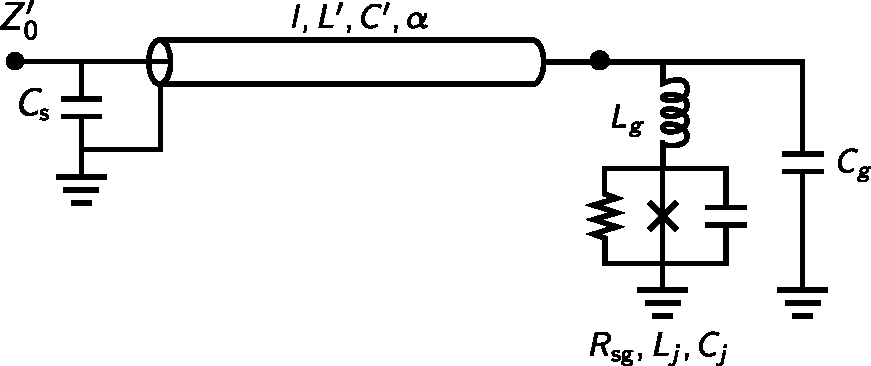
\includegraphics[width=.7\linewidth]{chapter-gJJ//figs/rfmodel}
	\caption[]{{\bf RF model for gJJ in cavity used for extraction of microwave parameters.}
		For the fitting procedure see \ref{sec:extraction}.
	}
	\label{fig:rfmodel}
\end{figure*}

\begin{figure*}[]
	\centering
	\includegraphics[width=\linewidth]{chapter-gJJ/figs/{si_calcavities.out}.pdf}
	\caption[]{{\bf Reference samples for extraction of microwave parameters.}
		\textbf{a,} Open-ended cavity measurement of the real (imaginary) part of the reflection coefficient plotted in blue (orange).
		Inset: Optical micrograph of junction area of the measured device (open end).
		\textbf{b,} Shorted-cavity measurement with same lead geometry as the actual gJJ sample.
		Inset: Optical micrograph of junction area of the measured device (connected to ground).
	}
	\label{fig:calcavities}
\end{figure*}

\begin{figure*}[]
	\centering
	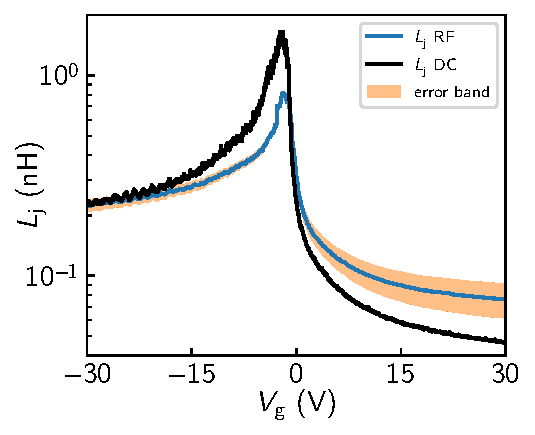
\includegraphics[width=0.5\linewidth]{chapter-gJJ/figs/fig3_supp_bands}
	\caption[]{\textbf{Josephson inductance extracted from RF and DC measurements, including error bands.}
		We plot here the same quantities as in Figure 3 of the main text but include error bands corresponding to minimum and maximum values originating from uncertainties in the circuit.
		The scales are identical to the plots in the main text.
	}
	\label{fig:figure3_bands}
\end{figure*}

\begin{figure*}[]
	\centering
	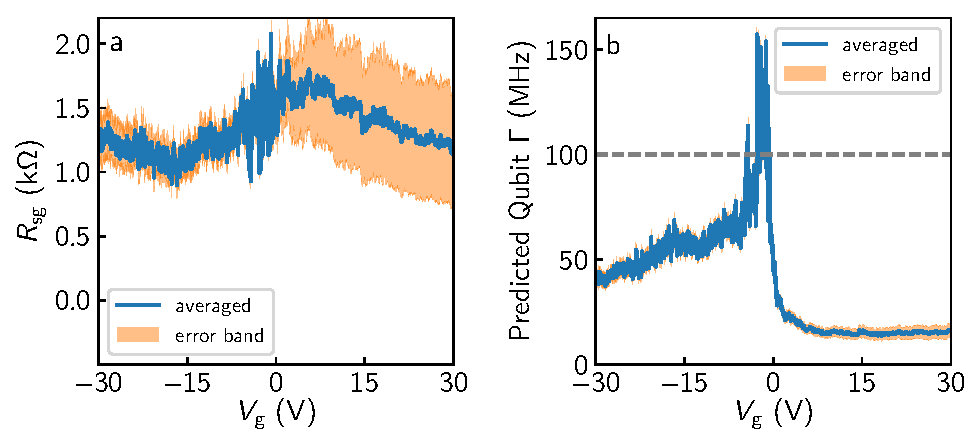
\includegraphics[width=\linewidth]{chapter-gJJ/figs/fig4_supp_bands}
	\caption[]{\textbf{Subgap resistance from microwave cavity measurements, including error bands.}
		We plot here the same quantities as in Figure 4 of the main text, but include error bands corresponding to minimum and maximum values originating from uncertainties in the circuit.
		The scales are identical to the plots in the main text.
		\textbf{a,} Subgap-resistance including error band.
		\textbf{b,} Corresponding linewidth of the hypothetical transmon with error band.
	}
	\label{fig:figure4_bands}
\end{figure*}

\begin{figure*}[]
	\centering
	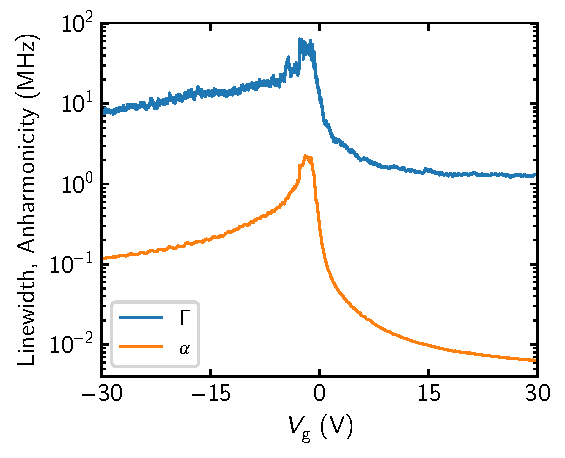
\includegraphics[width=.7\linewidth]{chapter-gJJ/figs/supp_anharmonicity_1.pdf}
	\caption{{\bf Anharmonicity and internal linewidth of current device, as described in \ref{sec:feasability}.}
		The calculated values of anharmonicity are always smaller than the measured linewidth meaning that this device cannot be considered a qubit in its current form.}
	\label{fig:anharm1}
\end{figure*}

\begin{figure*}[]
	\centering
	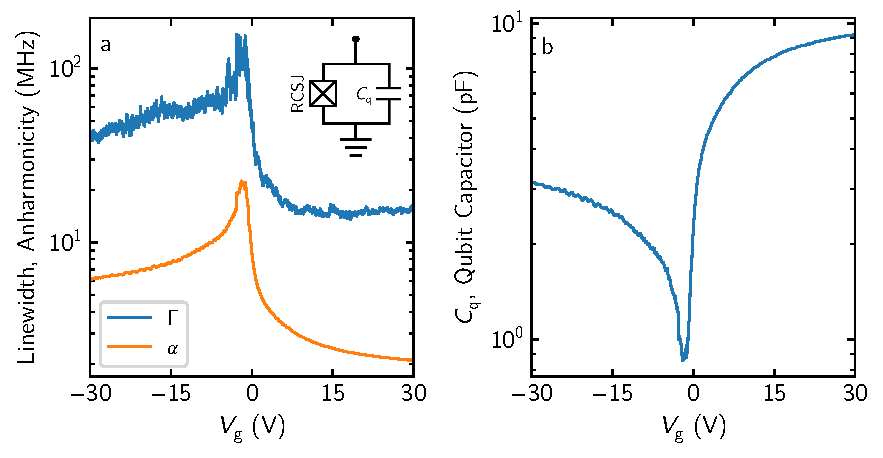
\includegraphics[width=.9\linewidth]{chapter-gJJ/figs/supp_anharmonicity_2.pdf}
	\caption{{\bf Anharmonicity and internal linewidth for design scenario A, as described in \ref{sec:scenA}.}
		\textbf{a,} We calculate the performance of the measured junction in a circuit shuch as the one shown in the inset.
		Setting the resonant frequency to $\omega_0 = 2\pi\times\SI{6}{GHz}$, we then calculate the anharmonicity and linewidth of this hypothetical device.
		Also in this case we find that calculated values of anharmonicity are always smaller than the linewidth.
		\textbf{b,} Required value of capacitance $C_\text{q}$ to maintain a resonant frequency of $\omega_0 = 2\pi\times\SI{6}{GHz}$ as a function of $V_\text{g}$}
	\label{fig:anharm2}
\end{figure*}

\begin{figure*}[]
	\centering
	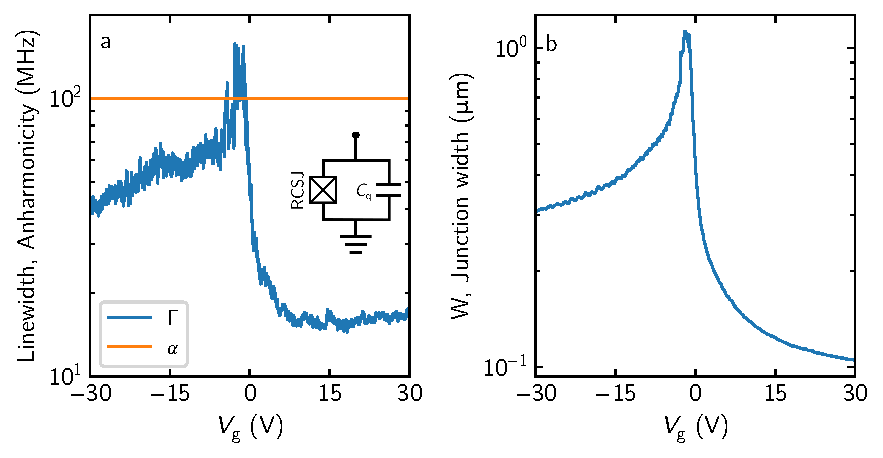
\includegraphics[width=.9\linewidth]{chapter-gJJ/figs/supp_anharmonicity_3.pdf}
	\caption{{\bf Anharmonicity and internal linewidth for design scenario B, as described in \ref{sec:scenB}.}
		\textbf{a,} We calculate the performance of a device whose capacitance and inductance are set by the requirement $\alpha = \SI{100}{MHz}$ and $\omega_0 = 2\pi\times\SI{6}{GHz}$.  This means scaling the junction width as a function of $V_\text{g}$.  The expected linewidth $\Gamma$ is shown along with the designed anharmonicity.
		\textbf{b,} Required junction width to maintain a resonant frequency of $\omega_0 = 2\pi\times\SI{6}{GHz}$ and $\alpha = \SI{100}{MHz}$ as a function of $V_\text{g}$.}
	\label{fig:anharm3}
\end{figure*}

\begin{figure*}[]
	\centering
	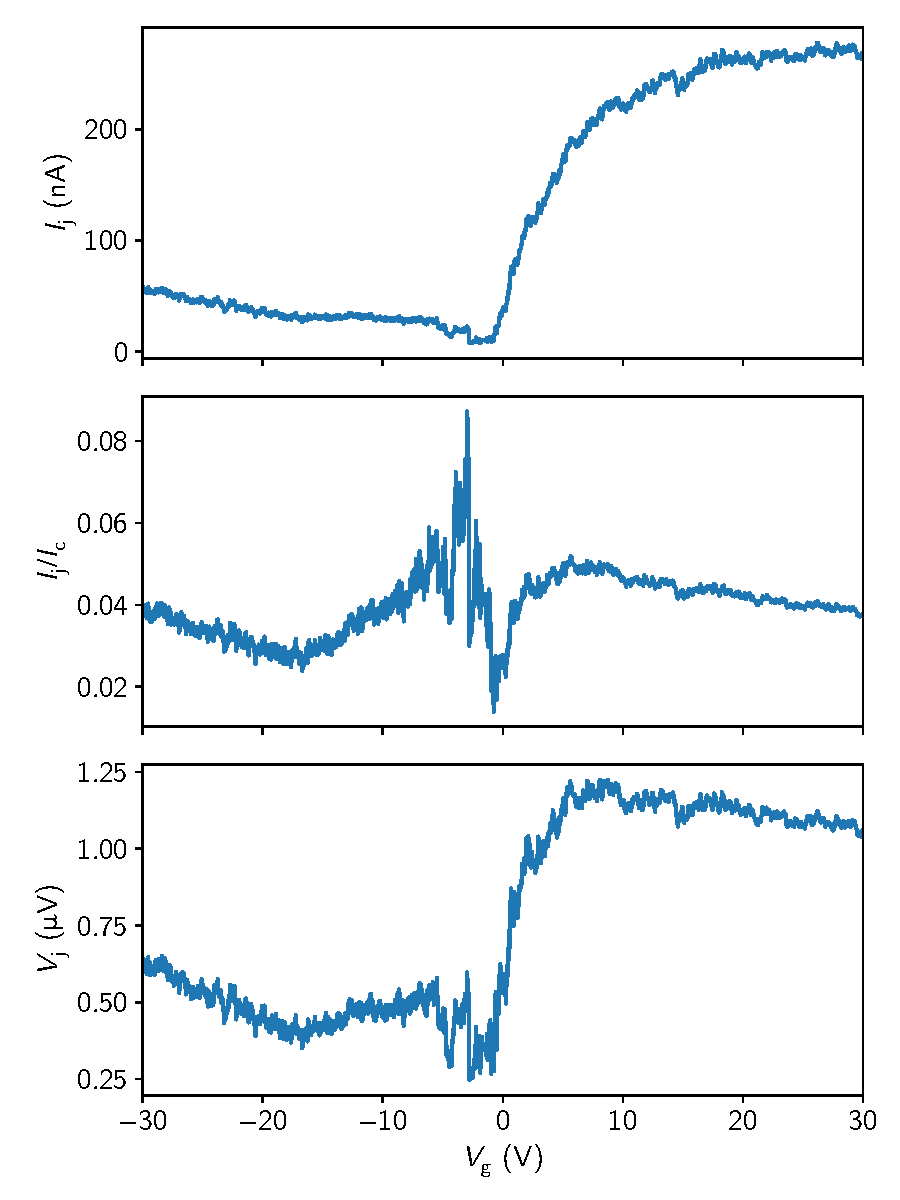
\includegraphics[width=0.6\linewidth]{chapter-gJJ/figs/supp_IjVj_plot}
	\caption{\textbf{Current and voltage amplitude at junction for measurement in Figure 2c of main text.}
		The input power at the device is estimated to be approximately \SI{-122}{dBm}.
		Currents are well below the measured critical current of the junction, even near the charge neutrality point.
		The average voltage across the junction induced by the microwave tone is lower than \SI{1}{\micro\volt}.
	}
	\label{fig:IjVj}
\end{figure*}

\begin{figure*}[]
	\centering
	\includegraphics[width=0.2\linewidth]{chapter-gJJ/figs/{resub_repeatdev_img_cmyk.out}.pdf}
	\caption{
		\textbf{Microscope image of second graphene superconducting junction.}
		The flakes around the device are hBN residues from the transfer process.
		Scale bar \SI{40}{\micro m}.
	}
	\label{fig:repeatdev_img}
\end{figure*}

\begin{figure*}[]
	\centering
	\includegraphics[width=\linewidth]{chapter-gJJ/figs/{si_2nddevice_cmyk.out}.pdf}
	\caption{\textbf{Observation of the Josephson inductance of a second graphene superconducting junction. a,}
		Differential resistance across the gJJ (Supplementary Figure \ref{fig:repeatdev_img}) for a wide gate voltage range.
		Dark blue denotes area of zero resistance.
		\textbf{b,} Normal state resistance of the gJJ versus gate voltage.
		\textbf{c,} Microwave spectroscopy of the device in the superconducting state versus gate voltage, plotted as the amplitude of the reflection coefficient $\lvert S_{11} \rvert$ after background subtraction.
		Remarkably, its performance is broadly similar to the main text device (see Figure 2 of main text), despite having been stored at room temperature in a nitrogen box for ten months before measurement.
	}
	\label{fig:repeatdev}
\end{figure*}

\begin{figure*}[]
	\centering
	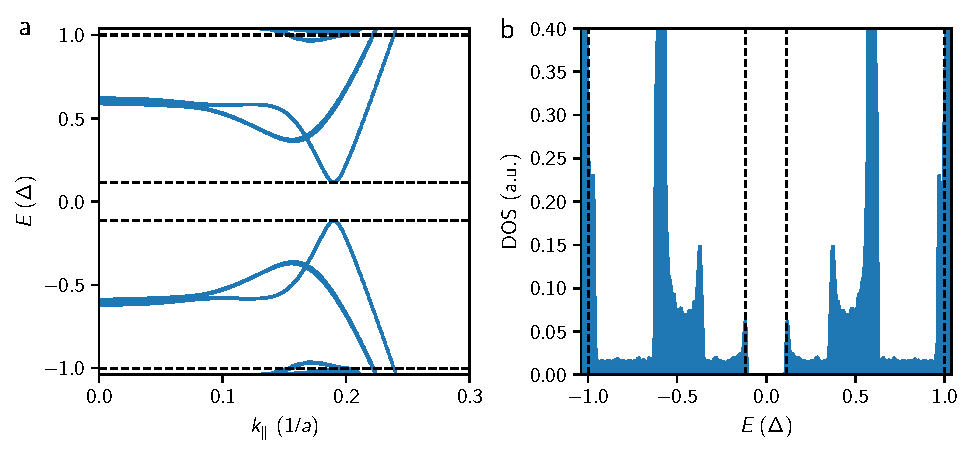
\includegraphics[width=\linewidth]{chapter-gJJ/figs/si_subgap_dos}
	\caption{{\bf Dispersion and density of states of a gJJ, as described in \ref{sec:subgap}.}
		{\bf a}, Simulated subgap dispersion for a graphene junction in the intermediate regime, $\Delta/E_\text{th}=1.542$ with $L_\text{N}=60$ and infinite lateral extension.
		Energy is scaled with respect to $\Delta$, $k_\parallel$ in terms of momentum parallel to the SN-interface.
		{\bf b}, By binning the energy dispersion we obtain the density of states as a function of energy.
		Various subgap peaks originating from ABS with high transverse momentum occur, while a hard gap remains, as indicated by the dashed horizontal lines.
	}
	\label{fig:subgap_dos}
\end{figure*}

\begin{figure*}[]
	\centering
	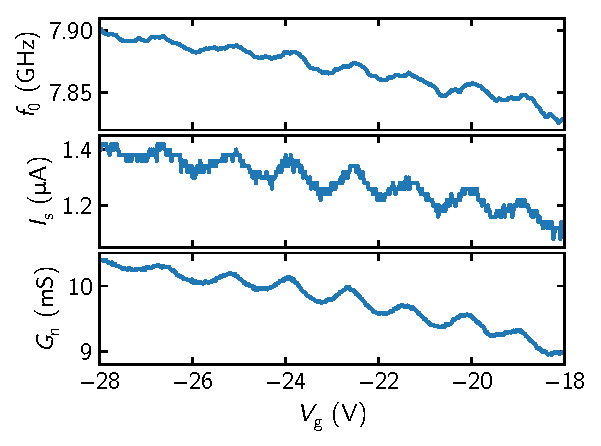
\includegraphics[width=.6\linewidth]{chapter-gJJ/figs/si_corr_osc}
	\caption{\textbf{Correlating oscillations in DC and RF measurements.}
		We observe reproducible and matching oscillations in-phase oscillations of resonance frequency, critical current and normal state conductance in the npn-regime.
		We attribute these to interfering electron waves partially reflected from the SN interfaces at the graphene-superconductor contacts:
		Since NbTiN slightly n-dopes the contact region (hence the asymmetry in $R_\text{n}$ as a function of gate voltage), pn-junctions form at the interface once the graphene is driven into the p-doped regime by the gate voltage.
		In the case of ballistic transport across the graphene sheet, the different charge carrier trajectories interfere with each other.
		Varying the gate voltage leads to a change in Fermi wavelength and hence an alternation of constructive and destructive interference, resulting in reduced and suppressed conductance, supercurrent, or inductance.
		This is akin to Fabry-P\'erot oscillations of light waves in free space, bound by two mirrors.
		The observation of these Fabry-P\'erot oscillations in graphene-based systems is uniformly taken as evidence of ballistic transport \cite{liangFabryPerotInterference2001,miaoPhaseCoherentTransportGraphene2007,youngQuantumInterferenceKlein2009,choMasslessMassiveParticleinabox2011,wuQuantumBehaviorGraphene2012,camposQuantumClassicalConfinement2012,rickhausBallisticInterferencesSuspended2013,benshalomQuantumOscillationsCritical2015,caladoBallisticJosephsonJunctions2015d,ametSupercurrentQuantumHall2016b,borzenetsBallisticGrapheneJosephson2016a,allenObservationElectronCoherence2017,zhuSupercurrentMultipleAndreev2018}.
		We therefore conclude that our device is also in the ballistic regime.
		We analyse these oscillations in Supplementary Figure \ref{fig:fabry-perot}.
	} 
	\label{fig:quantum_osc}
\end{figure*}

\begin{figure*}[]
	\centering
	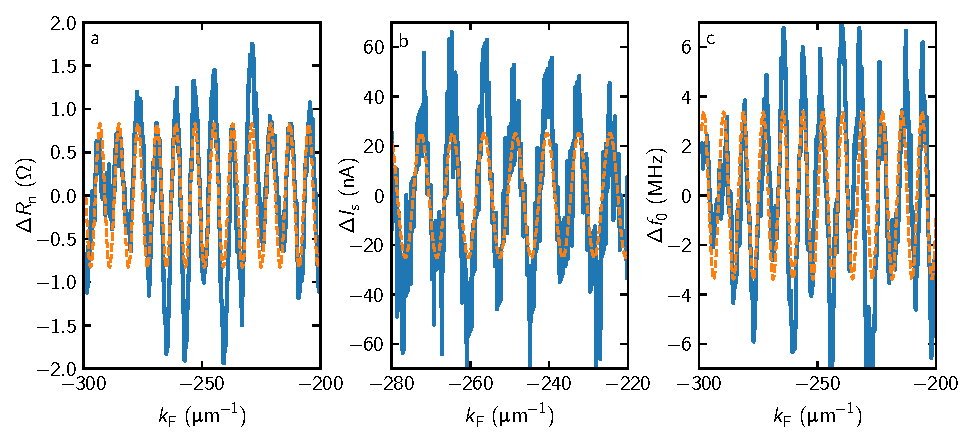
\includegraphics[width=\linewidth]{chapter-gJJ/figs/si_fabryperot}
	\caption{{\bf Fabry-P\'erot oscillations in ballistic gJJ.}
		We observe FP oscillations in \textbf{(a)} $R_\text{n}$, \textbf{(b)} $I_\text{c}$ and \textbf{(c)} $f_0$.
		We can extract the length of the resonant cavity by fitting our oscillating signal with a sine, according to the resonance condition $2L_\text{c} = m\lambda_\text{F}, m\in\mathbb{N} \rightarrow 2L_\text{c} k_\text{F} = 2\pi m$.
		After subtracting a slowly varying background with a third-order polynomial \cite{caladoBallisticJosephsonJunctions2015d}, the fits for $R_\text{n}$, $I_\text{c}$ and $f_0$ (orange lines) independently yield $L_\text{c}\approx \SI{390}{nm}$.
		This suggests a contact interface barrier of no more than \SI{55}{nm} on each side.
		We can thus take $L_\text{c}$ as a lower bound for the free momentum scattering and the phase coherence lengths, i.e. $l_\text{mfp},\xi>L_\text{c}$.        }
	\label{fig:fabry-perot}
\end{figure*}

\begin{figure*}[]
	\centering
	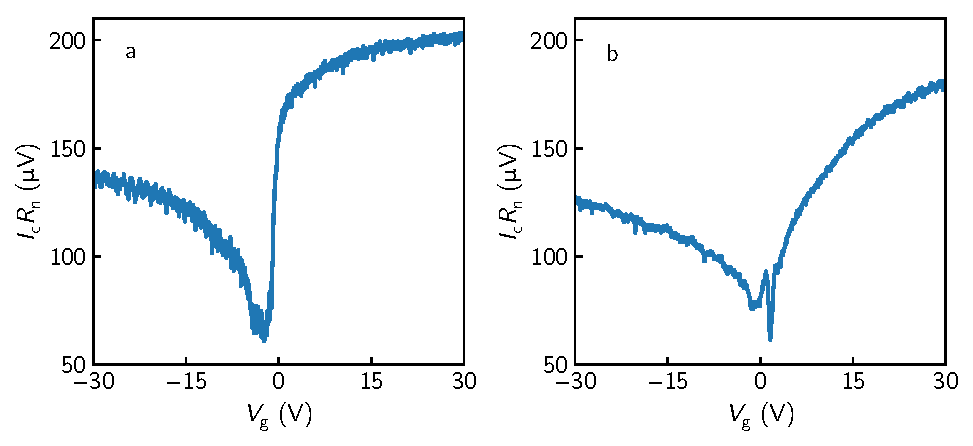
\includegraphics[width=\linewidth]{chapter-gJJ/figs/si_icrn}
	\caption{{\bf $I_\text{c} R_\text{n}$ product of gJJ devices.}
		The $I_\text{c} R_\text{n}$ product in Josepshon junctions is directly proportional to the gap voltage \cite{tinkhamIntroductionSuperconductivity1996}, with $I_\text{c} R_\text{n}\geq2.08\Delta/e$ in the case of ballistic graphene junctions \cite{titovJosephsonEffectBallistic2006b,cuevasSubharmonicGapStructure2006a}.
		\textbf{a,} In our main device, this quantity saturates at approximately \SI{200}{\micro V} for high n-doping, drops to \SI{50}{\micro V} around CNP, and reaches up to \SI{130}{\micro V} for high p-doping.
		We take the small dependence on gate voltage in high doping regime as further indication of ballistic transport \cite{mizunoBallisticlikeSupercurrentSuspended2013a,zhuSupercurrentMultipleAndreev2018}.
		Taking the bulk gap of the leads to be $\Delta=1.764 k_\text{B} T_\text{c} = \SI{2}{meV}$, our maximum $I_\text{c} R_\text{n}=0.1\Delta$ which is much lower than the theoretically expected value.
		We attribute this to reduced contact transparency and our junction being in the long regime, where the Thouless energy $E_\text{th}=hv_\text{F}/L < \Delta $ is the dominant energy scale, limiting $I_\text{c} R_\text{n}$ \cite{dubosJosephsonCriticalCurrent2001}.
		Our observation matches that of various other groups \cite{mizunoBallisticlikeSupercurrentSuspended2013a,benshalomQuantumOscillationsCritical2015,borzenetsBallisticGrapheneJosephson2016a,zhuSupercurrentMultipleAndreev2018}.
		\textbf{b,} In contrast, the additional device lacks the saturating behaviour, and exhibits a lower $I_\text{c}R_\text{n}$ product.
		This, in addition to the absence of FP oscillations, leads us to conclude that the latter device is non-ballistic, possibly due to a slightly longer normal region, or residual dirt (such as bubbles) in the graphene channel.
	}
	\label{fig:icrn}
\end{figure*}

\begin{figure*}[]
	\centering
	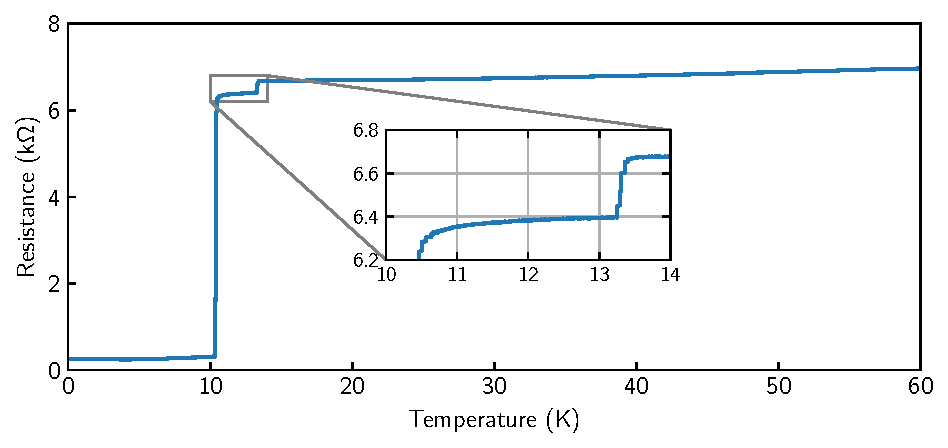
\includegraphics[width=.7\linewidth]{chapter-gJJ/figs/si_cooldown_tc}
	\caption{{\bf Critical temperature of MoRe and NbTiN.}
		Resistance versus temperature of the gJJ sample, measured during the initial cooldown, for a current bias of \SI{1}{\micro A} without any gate voltage applied.
		The two jumps at \SI{10.5}{K} and \SI{13.2}{K} correspond to the critical temperature of MoRe and NbTiN, respectively.
		Below $T_\mathrm{c,MoRe}$, we measure a residual resistance of \SI{250}{\ohm}, which corresponds to the graphene sheet resistance for $V_\text{g}=\SI{0}{V}$.}
	\label{fig:critical_temp}
\end{figure*}

% \clearpage
%%%%%%%%%%%%%%%%%%%%%%%%%%%%%%%%%%

\begin{table*}
	\begin{center}
		\begin{tabular}{|c|c|}
			\hline 
			$l$ (TL length) & \SI{6119}{\micro\meter} \\ 
			\hline 
			$C'$ (Capacitance per unit length) & \SI{0.14848}{nF/m} \\ 
			\hline 
			$L'$ (Total inductance per unit length) & \SI{0.619838}{\micro\henry/m} \\ 
			\hline
			$C_\text{s}$ (Shunt coupler capacitance) & $\sim$\SI{27}{pF} \\ 
			\hline 
			$Z_0$ (TL Characteristic impedance) & \SI{64.611}{\ohm} \\
			\hline 
			$Z'_0$ (Reference impedance) & \SI{50}{\ohm} \\
			\hline 
			$v_\text{ph}$ (Phase velocity in TL) & \SI{1.04238e8}{m/s} = 0.3477 $c_0$ \\ 
			\hline
			$L'_\text{g} = \frac{\mu_0}{4}\frac{K({k'_0}^2)}{K({k_0}^2)}$ (Geometric inductance per unit length) & \SI{0.4277}{\micro\henry/m} \\ 
			\hline
			$L'_\text{k}$ (Kinetic inductance per unit length) & \SI{0.1922}{\micro\henry/m} \\ 
			\hline
			$L'_\text{k}/L'$ (Kinetic inductance fraction) & \num{0.31} \\ 
			\hline
			$L_\text{g}$ (Geometric inductance of junction leads) & \SIrange[range-phrase=--]{70}{100}{pH} \\ 
			\hline
			$C_\text{g}$ (Geometric capacitance of junction leads) & \SI{4.7}{fF} \\ 
			\hline
			$C_\text{j}$ (gJJ capacitance) & \SI{2}{fF} \\ 
			\hline
			$\alpha$ (Attenuation at \SI{8.1089}{GHz}) & \SI{0.006073}{\per\metre} \\ 
			\hline
		\end{tabular}
		\caption{\bf Transmission line, coupler and junction parameters with kinetic inductance correction included, as described in \ref{sec:extraction}.}
		\label{tab:tlpars}
	\end{center}
\end{table*}

\clearpage
%%%%%%%%%%%%%%%%%%%%%%%%%%%%%%%%%%



\references{dissertation}


%\newchapstyle
\chapter{Current phase relations of graphene Josephson junctions in microwave circuits}
\label{chap:gJJ-CPR}

\blfootnote{
	\color{title}
	This chapter is based on previously unpublished data of the devices presented in Chapter~\ref{chap:gJJ}.
	%
	Data and code to reproduce the calculations and figures presented here can be found on Zenodo~\cite{schmidtDataCodeCurrent2020}.
}

\begin{abstract}
	We perform extensive analysis of graphene Josephson junctions embedded in microwave circuits.
	%
	By comparing a diffusive junction at \SI{15}{\milli\kelvin} with a ballistic one at \SI{15}{\milli\kelvin} and \SI{1}{\kelvin}, we are able to reconstruct the current-phase relation.
\end{abstract}

%% Start the actual chapter on a new page.
\newpage

\section{Introduction}

Josephson junctions are widely used in high frequency applications, such as quantum information processing and sensing.
%
There, they are being exploited as nonlinear inductors.
%
However, their nonlinear character can significantly differ from junction to junction depending on the intrinsic properties of the current-phase relation.
%
For the use of JJs in superconducting quantum information circuits, the junction nonlinearity has a major effect on the circuit requirements and capabilities~\cite{kringhojAnharmonicitySuperconductingQubit2018}.
%
While the CPR of gJJs has been studied in the DC regime before~\cite{englishObservationNonsinusoidalCurrentphase2016,nandaCurrentPhaseRelationBallistic2017}, and gJJs have been successfully incorporated in RF circuits~\cite{schmidtBallisticGrapheneSuperconducting2018,krollMagneticFieldCompatible2018,wangCoherentControlHybrid2019}, the influence of the non-sinusoidal CPR has not been studied in this regime.

Here, we analyze the influence of the CPR on the microwave performance of RF-circuit embedded gJJ and compare the influence of scattering transport and temperature.
%
Our circuit design allows in-situ, and even simultaneous, even DC and RF measurements, providing us with various measurement types to compare.
%
The results show the usefulness of combining DC and RF in the same circuits for funamental research on Josephson junction physics.

\section{Circuit characterization}

Our circuit consists of a DC-bias microwave cavity formed by a coplanar waveguide (CPW) which is shunted by a large capacitor at the input, and shorted to ground on the far end by a gate-voltage ($V_g$) tunable graphene Josephson junction (gJJ), cf. Fig.\ref{fig:figure1}(a) and Refs.~\cite{schmidtBallisticGrapheneSuperconducting2018,schmidtCurrentDetectionUsing2020,bosmanBroadbandArchitectureGalvanically2015c}.
%
The superconducting base layer and shunt capacitor metal layers consist of DC-sputtered molybdenum-rhenium (MoRe) on a sapphire substrate, while the shunt capacitr dielectric layer is PECVD-SiN.
%
The circuit is connected via a bias-T, allowing both DC and RF characterization in the same setup, and mounted on the millikelvin plate on a dilution refrigerator.
%
The gate voltage lead is fed through a shunt capacitor of the same geometry as the capacitor at the input in order to suppress RF radiation leaking in through or out of the gate line.

We measured two separate devices with nominally identical microwave circuits and junction designs:
%
One of the devices exhibited signatures ballistic DC-transport, which we will refer to as the \textit{ballistic device}, which is the device presented in the main text of Ref.~\cite{schmidtBallisticGrapheneSuperconducting2018}.
%
The other one, in lack of such features, will be called \textit{diffusive device}, and corresponds to the reference sample of Ref.~\cite{schmidtBallisticGrapheneSuperconducting2018}.
%
Both gJJ were designed to be \SI{5}{\micro\meter} wide and separate the NbTiN leads by a length of \SI{500}{\nano\meter}.
%
Gate tunability is achieved by placing a third NbTiN lead extending over the entire gJJ, separated by a bilayer of HSQ.

We extract the DC circuit parameters by applying a bias current to the JJ, using the CPW as a long capacitive lead.
%
All DC lines were equipped with $\pi$-filters in the room temperature battery powered electronics, as well as copper powder and two-stage RC filters thermally anchored to the millikelvin stage of the dilution refrigerator.
%
When exceeding a critical current, the JJ switches from the zero-voltage to the resistive state.
%
We record this switching current $I_s$ for varying gate voltages, as depicted in the top row of Fig.~\ref{fig:figure1} for the two devices at two different temperatures.
%
The DC switching current of the diffusive device ranges from a few \SI{100}{\nano\ampere} to \SI{5.5}{\micro\ampere}, similar to the hot ballistic device.
%
At base temperature, the maximum $I_s$ of the ballistic device reaches \SI{7.5}{\micro\ampere} for $V_g>V_{\rm CNP}$, while for p-doping the enhancement in $I_s$ is significantly smaller.

For high frequency signals, i.e. a few \si{\giga\hertz}, the gJJ behaves as a nonlinear inductor, with Josephson inductance
%
\begin{align}
L_J = \frac{\Phi_0}{2\pi}\left(\diff{I_J}{\delta}\right)^{-1},
\end{align}
%
where $\Phi_0$ is the magnetic flux quantum and $I_J(\delta)$ the current phase relation (CPR) between the phase difference $\delta$ across the JJ between two superconducting banks and the corresponding supercurrent $I_J$ flowing through the junction.
Depending on the impedance of the gJJ at the circuit resonance frequency, $Z_J=i\omega_0 L_J$, the fundamental mode hosted by the gJJ-terminated CPW varies between a $\lambda/2$ wave for $Z_J\rightarrow0$ and $\lambda/4$ for $Z_J\rightarrow\infty$.
%
Since the supercurrent in our gJJs cannot be fully suppressed, the maximum $L_J\lessapprox\SI{1}{\nano\henry}$, thus $Z_J\lessapprox1 <  Z_0\approx\SI{50}{\ohm}$ with the CPW impedance $Z_0$.
%
Our devices thus remain in the $\lambda/2$-resonator regime.

The device response is measured by recording the reflection coefficient $S_{11}$ using a vector network analyzer, which excites the device through a series of attenuators and a directional coupler, and measuring the reflected signal, amplified by low noise cryogenic and room temperature HEMTs. 
%
We fit the response using an analytical model (cf. Supplementary Sec.~\ref{sec:extraction}).
%
The measurements show a gate-tunable resonance frequency $f_0$ between \SIrange{7.0}{8.2}{\giga\hertz}, comparable for both devices, cf. bottom row of Fig.~\ref{fig:figure1}.
%
Due to the inverse nature of junction current and inductance, the large changes in $I_s$ for $V_g>V_{\rm CNP}$ only lead to minor changes in $f_0$ when comparing the hot and cold ballistic device.
%
On the other hand, even small changes in the significantly smaller $I_s$ for $V_g<V_{\rm CNP}$ significantly reduce $f_0$ in this regime.

\begin{figure}
	\centering
	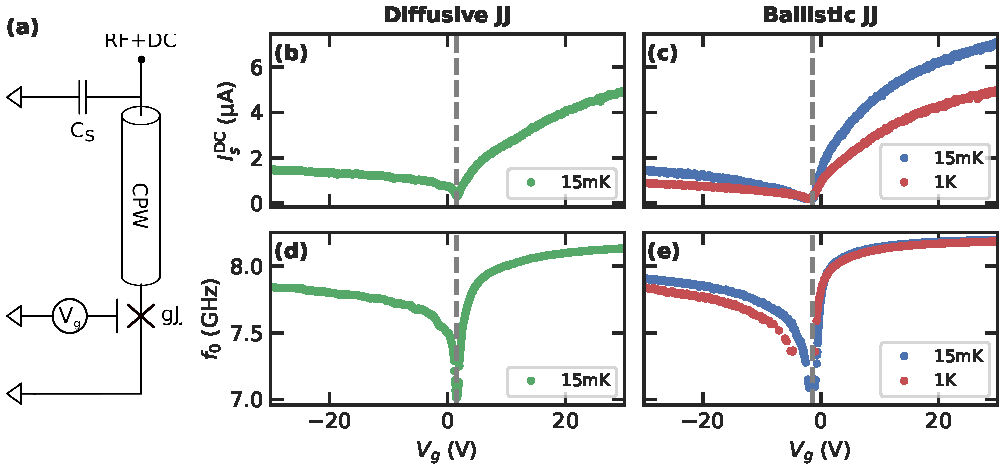
\includegraphics[width=\linewidth]{chapter-gJJ-CPR/figs/Figure1}
	\caption{
		\textbf{A graphene Josephson junction embedded in a DC bias microwave circuit.}
		%
		\textbf{(a)} Measurement schematic.
		%
		The gJJ shorts a coplanar waveguide transmission line to ground, which forms a gate-tunable $\lambda/2$-resonator.
		%
		\textbf{(b-e)} Switching currents (top row) for the diffusive \textbf{(b)} and ballistic Josephson junction \textbf{(d)}, at base-temperature of \SI{15}{\milli\kelvin} (blue) and at \SI{1}{\kelvin} (red).
		%
		Bottom row: Resonance frequencies versus gate voltage for the diffusive \textbf{(c)} and ballistic \textbf{(e)} device.
		%
		The gate-tunable Josephson inductance changes the boundary condition of the $\lambda/2$-resonator, thus changing the resonance frequency of the circuit.
		%
		Dashed grey lines indicate the charge neutrality point
	}
	\label{fig:figure1}
\end{figure}

\section{Measuring the Josephson inductance in DC and RF}

The resonance frequency of a $\lambda/2$-resonator shorted to ground by a Josephson inductance can be approximated by
\begin{align}
f_0\left(I_b,I_c\right) = f_{\lambda/2} \frac{L_r+L_J\left(I_b, I_c\right)}{L_r +  2L_J\left(I_b, I_c\right)}
\label{eq:Pogorzalek}
\end{align}
%
with $L_r$ the bare CPW inductance and $f_{\lambda/2}$ the resonance frequency of the CPW without the JJ, see Supplementary Material Sec.~\ref{sec:validity}.
%
$I_b$ is the bias current flowing through CPW and the JJ, $I_c$ the critical current of the JJ.
%
We can immediately see that for small $L_J$, $f_0=f_{\lambda/2}$, while for $L_J\gg L_r$, $f_0=f_{\lambda/2}/2$.
%
Assuming a purely sinusoidal current-phase relation,
%
\begin{align}
I_J(\delta) = I_c\sin\delta,
\label{eq:CPR-sin}
\end{align}
%
the Josephson inductance can be extracted from the current phase relation via
%
\begin{align}
L_J = \frac{\Phi_0}{2\pi I_c \cos\delta}.
\label{eq:LJsin}
\end{align}
%
Depending on the exact shape of the CPR however, $L_J$, and with it $f_0$ can significantly deviate from the above equations, cf. Supplementary Fig.~\ref{fig:SMinfluence}.
%
Specifically, the CPR of gJJ are known to exhibit forward-skewing, where the skew is defined as the deviation of the CPR maximum from phase $\pi/2$, $S=2\delta_{\rm max}/\pi -1$.

As depicted in Fig.\ref{fig:figure2}, we fit the RF-measured $f_0$ versus the DC-measured $I_s^{\rm DC}$ using Eq.~\ref{eq:Pogorzalek} assuming a sinusoidal CPR, shown by the black dashed line.
%
Here, we assumed $\delta=0$ because the DC bias port was shorted to ground during measurement, and the RF excitation merely oscillates the phase around zero.
%
The fit converges for both the diffusive and the “hot” ballistic device.
%
On the other hand, at \SI{15}{\milli\kelvin}, the ballistic device exhibits multi-valued $f_0\left(I_s\right)$, as the resonance frequency and switching current follow different trends for p- and n-doping.
%
This is a first indication of a deviation of the CPR from Eq.\ref{eq:CPR-sin}.

%% How to formulate this in a good way?
%% DC-Is and assumption of sinusoidal CPR leads us to an estimated DC-Lj.
%% This value is smaller than the actually measured Lj
%% This can only be if the CPR is forward skewed because this enhances the true Lj while keeping Ic the same for the two cases.
%% To get the same Lj as for a sinusoidal CPR, DC-Is would need to be smaller.? But according to Figs1.2, 1.3 it would need to be larger???
%% TODO!

\begin{figure}
	\centering
	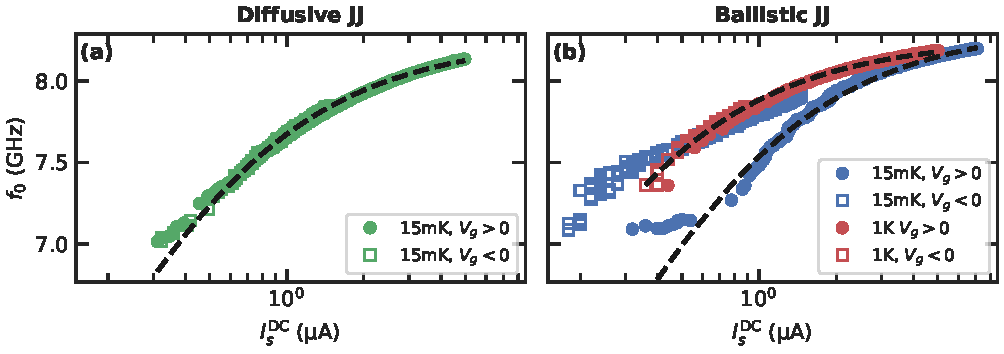
\includegraphics[width=0.583\linewidth]{chapter-gJJ-CPR/figs/Figure2}
	\caption{
		\textbf{Resonance frequency vs switching currents for two different gJJ devices.}
		%
		Both the diffusive device at low temperature \textbf{(a)} and the ballistic device at \SI{1}{\kelvin} (\textbf{(b)}, red) show monotonically increasing $f_0$ versus DC-extracted switching currents.
		%
		In contrast, for low temperatures, the ballistic gJJ (\textbf{(b)}, blue) exhibits multi-valued $f_0\left(I_s\right)$ for gate voltages larger (full circles) and smaller (empty squares) than the charge neutrality point.
		%
		The	multivalued behavior in the ballistic device at low temperature indicates a strong nonsinusoidal CPR and only allows for a fit for $V_g>0$, while this is not observed at higher temperature or for the diffusive device.
		%
		Dashed lines correspond to fits to Eq.~\ref{eq:Pogorzalek}.
	}
	\label{fig:figure2}
\end{figure}

We can additionally directly compare the estimates for the junction critical current from our DC measurement, $I_s^{\rm DC}$, with the value calculated from our RF measurement of the resonance frequency via Eq.~\ref{eq:LJsin}, $I_c^{\rm RF}=I_c\left(L_J\left(f_0\right)\right)$. 
%
As shown in Fig.~\ref{fig:figure3}, our devices exhibit tunable supercurrent over almost two orders of magnitude range.
%
In the diffusive device, $I_s^{\rm DC}$ and $I_c^{\rm RF}$ match closely, but small deviations at the low and high end are visible, with $I_c^{\rm RF}$ resulting in values larger than expected from DC.
%
Similarly, the DC measurements of the ballistic device at \SI{1}{\kelvin} underestimate the critical current as extracted from RF for small values of $I_s^{\rm DC}$, but match remarkably well everywhere else.
%
At first glance, any forward skew in the CPR should lead to a drop in CPR slope.
%
Therefore, for the same value of $I_c$, $L_J$ should increase and $I_s^{\rm RF}<I_s^{\rm DC}$.
%
However, our fit results in the opposite behavior, cf. Supplementary Fig.~\ref{fig:SMinfluence}:
%
The fit model returns a larger $I_c$ than expected for a sinusoidal CPR, given that the data to be fitted has an underlying forward-skewed CPR.
%% I think I have this written down somewhere in one of the ipynb files?

At a temperature of \SI{15}{\milli\kelvin}, the ballistic device deviates significantly from the DC-calculations, especially at low currents and $V_g<0$.
%
Deviations at large $I_c$ are less obvious, presumably due to the fact that in this regime, $L_J \ll L_r$ and the Josephson inductance has only minor effect on $f_0$. \textbf{TODO: ERROR PROPAGATION FOR FIG 1.3!!! IT DEPENDS ON df0, AND ALSO ON dfr AND dLr!!!}

This shows that extrapolation of a value for $L_J$ at microwave frequencies from DC measurements can lead to severe discrepancies.
%
In order to examine the underlying mechanisms further, we continue by studying the power and bias current dependence of our circuit.

\begin{figure}
	\centering
	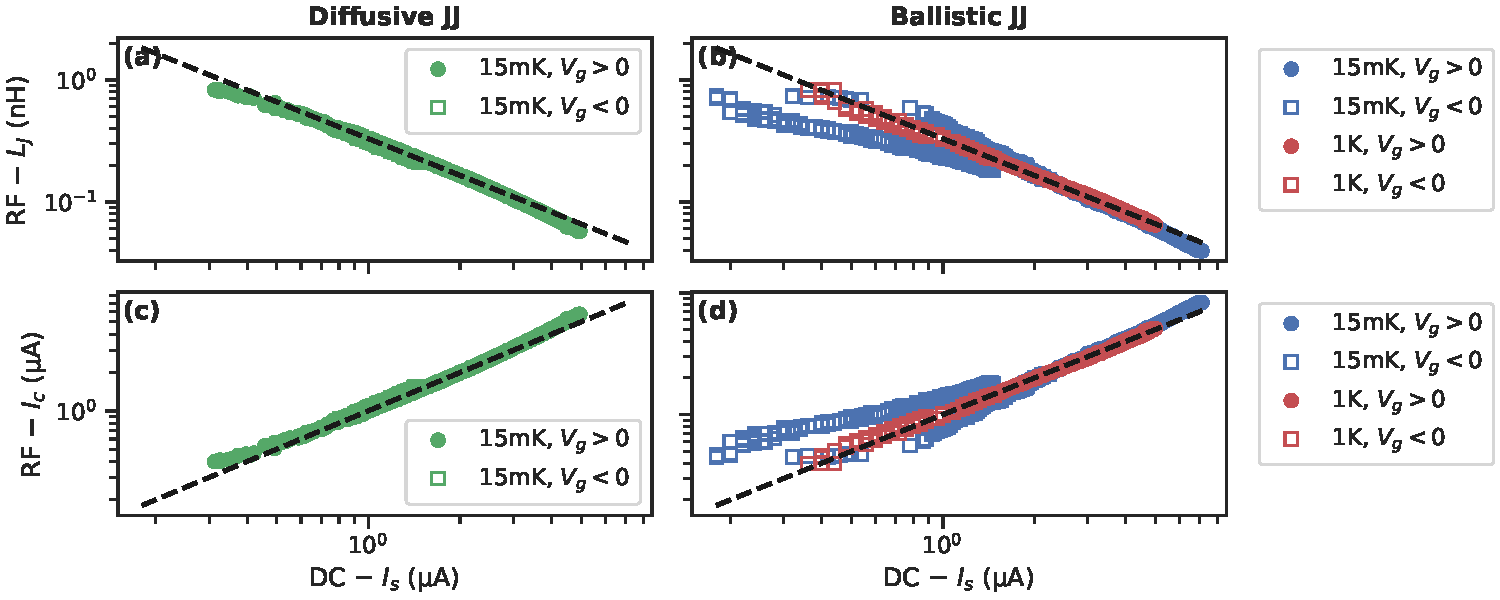
\includegraphics[width=0.583\linewidth]{chapter-gJJ-CPR/figs/Figure3}
	\caption{
		\textbf{Comparing switching and critical currents.}
		%
		RF-extracted critical current versus DC-measured switching current for the diffusive device at \SI{15}{\milli\kelvin} \textbf{(a)} and the ballistic device at \SI{15}{\milli\kelvin} and at \SI{1}{\kelvin} (\textbf{(b)}, blue and red, respectively).
		%
		Dashed line corresponds to DC-measured $I_s$.
		%
		Both scattering in the JJ as well as elevated temperatures reduce the deviation from RF and DC data.
		\textbf{TODO: ERROR PROPAGATION FOR FIG 1.3!!! IT DEPENDS ON df0, AND ALSO ON dfr AND dLr!!!}
	}
	\label{fig:figure3}
\end{figure}

\section{Anharmonicity of a gJJ RF circuit}

The nonlinear inductance of a Josephson junction consequently introduces nonlinear behaviour of the overall circuit.
%
Depending on the exact circuit design, this nonlinearity is more or less diluted, yet finite so-called anharmonicity, i.e. deviation from the ideal case of pure LC-resonator behavior, remains.

We can observe the anharmonicity of our gJJ-terminated DC bias circuit by performing $S_{11}$ measurements at high drive powers, as shown in Fig.~\ref{fig:figure4}.
\textbf{TODO: What was the drive power at which all the other measurements were performed?}
\textbf{TODO: Update arXiv references}

The anharmonicity of a CPW shorted to ground by a Josephson junction is given by~\cite{wilsonPhotonGenerationElectromagnetic2010b,zhouHighgainWeaklyNonlinear2014}
\begin{align}
\beta=-\frac{f_0}{2} \left(\frac{L_J}{L_r+L_J}\right)^3\ ,
\label{eq:anharmonicity}
\end{align}
%
where we have followed the same notation as in the earlier equations.
%
However, in the case of a non-sinusoidal CPR, the anharmonicity is reduced due to the increased CPR slope, resulting in
\begin{align}
\beta^\prime = \beta \left( 1-\frac{3}{4}\frac{\sum_i\tau_i^2}{\sum_i\tau_i}\right) \rightarrow \beta \left( 1-\frac{3}{4}\tau \right)
\label{eq:anh_nonsin}
\end{align}
%
where the limes holds for an average $\tau$ of the ensemble of transmission channels~\cite{kringhojAnharmonicitySuperconductingQubit2018}.

A more suitable measurement would have been to perform two-tone spectroscopy with a fixed-frequency pump tone with variable power, and a low-power swept probe tone, since this would avoid bifurcation and yield a direct measurement of the anharmonicity from the frequency shift per photon.
%
However, such a setup was not available at the time.


Non-linear dissipation is absent in SIS JJ circuits ~\cite{boakninDispersiveMicrowaveBifurcation2007}, but is necessary for our setup to get good agreement of data and model at high drive powers.
%
Dissipation mechanisms could include heating, dielectric losses, or subgap losses!
%
Maybe what we observe here are the subgap states!!~\cite{fuechsleEffectMicrowavesCurrentPhase2009,dassonnevilleDissipationSupercurrentFluctuations2013}
%
We populate them as we increase the drive power, resulting in an increase in internal loss rate, cf. Supplementary Fig.~\ref{fig:SMFig-lossrates}.
%
Difficult to separate from the dielectric circuit losses.
%
However, dielectric volume is only present at voltage nodes, where these effects should not play a significant role.
%
Heating of the circuit itself is unlikely due to the close match between data and model, and the fact that $f_0$ should tune significantly stronger, since $I_c$ should also be reduced by the heat which can have strong influence on $f_0$, c.f. Fig.~\ref{fig:figure1}.

\begin{figure}
	\centering
	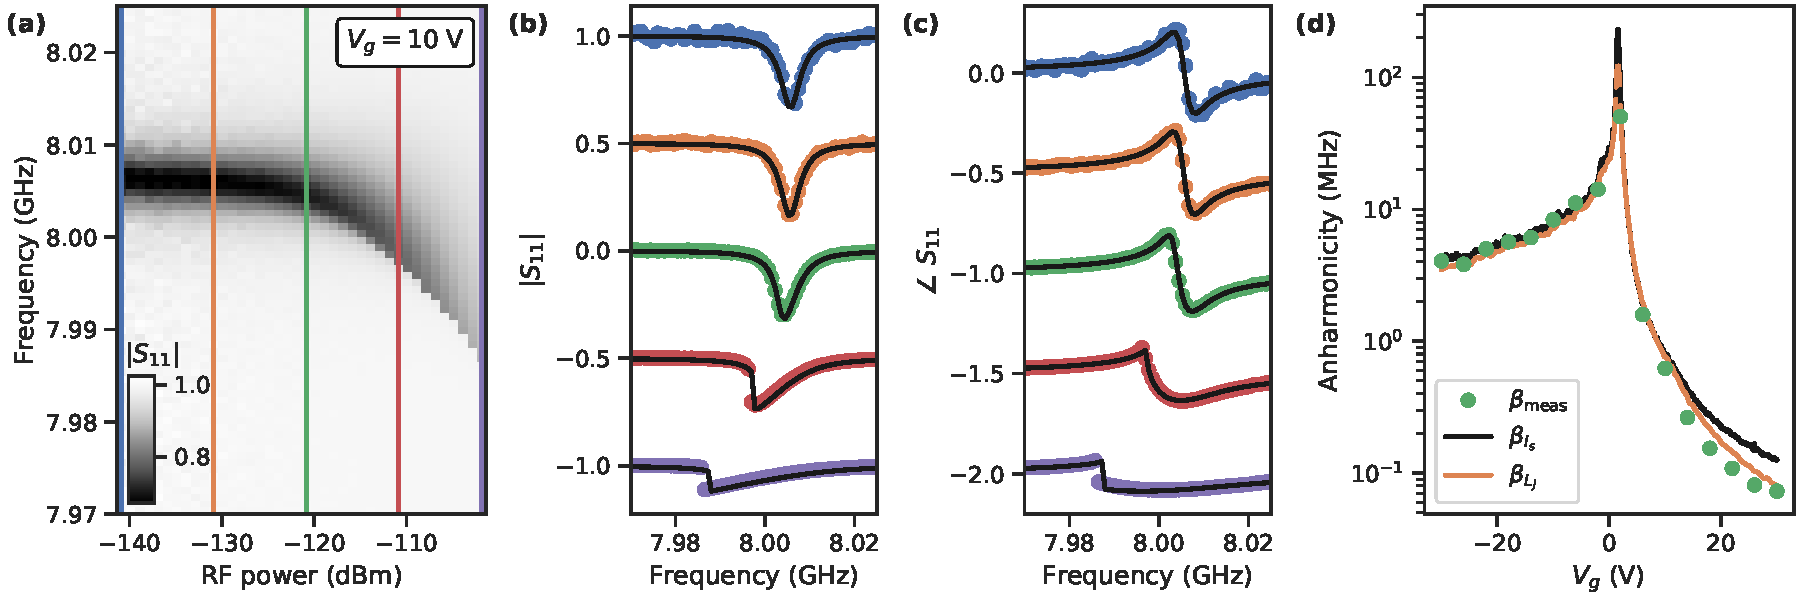
\includegraphics[width=\linewidth]{chapter-gJJ-CPR/figs/Figure4}
	\caption{
		\textbf{Power dependence of a nonlinear microwave device with diffusive gJJ.}
		%
		\textbf{(a)} Absolute value of the reflection coefficient $S_{11}$ versus frequency for increasing drive power.
		%
		Due to the Kerr nonlinearity, the resonator experiences a downshift and bifurcation at elevated drive powers.
		%
		Solid lines indicate linecuts in \textbf{(b)} and \textbf{(c)}.
		%
		\textbf{(b-c)} Absolute value \textbf{(b)} and phase \textbf{(c)} of $S_{11}$ for varying drive power as indicated in \textbf{(a)}.
		%
		Black lines are fits.
		%
		\textbf{(d)} Anharmonicity vs gate voltage.
		%
		Dots: data as extracted from fits as in \textbf{(b-c)}, orange line: model using $I_s^{\rm DC}$, green: model using $L_J$.
		%
		The overestimation of the anharmonicity of the $I_s^{\rm DC}$ for high gate voltages is consistent with and confirms a non-sinusoidal CPR.
	}
	\label{fig:figure4}
\end{figure}

\section{Reconstructing the current phase relation}

A more realistic model for the CPR of our devices than Eq.~\ref{eq:CPR-sin} is the one for a ballistic point contact as a function of transparency $\tau$ and temperature $T$:
%
\begin{align}
I_J(\delta,\tau,T) = \frac{\pi\Delta_0}{2 e R_n} \frac{\sin\delta}{\sqrt{1 - \tau \sin^2\delta / 2}} \tanh\left[\frac{\Delta_0}{k_B T} \sqrt{1 - \tau \sin^2\delta / 2}\right]\ ,
\label{eq:CPR-ball}
\end{align}
%
with the superconducting energy gap $\Delta_0$, the Boltzmann constant $k_B$ and normal state resistance $R_n= R_q/N = h/(Ne^2)\approx \SI{25.812}{\kilo\ohm} / N$~\cite{golubovCurrentphaseRelationJosephson2004a}.
%
Here, $R_q$ denotes the quantum Hall resistance and $N$ the number of conducting channels.
%
With a normal state resistance of or devices ranging between \SIrange{35}{350}{\ohm} (depending on gate voltage), we estimate around 74 to 740 conducting channels.
%
This justifies the use of a single transparency parameter $\tau$ that is the average of all the other channels.

average channel transmission 0.17 and 0.88
This corresponds to a forward skew of 0.03 and 0.34 for the diffusive and ballistic device, respectively, comparable to measurements from DC-measurements of the CPR~\cite{englishObservationNonsinusoidalCurrentphase2016,nandaCurrentPhaseRelationBallistic2017}.
%
%$I_c(\tau,T)=\underaccent{\delta}{\max} \left[I_J(\delta,\tau,T)\right]$
%

\begin{figure}
	\centering
	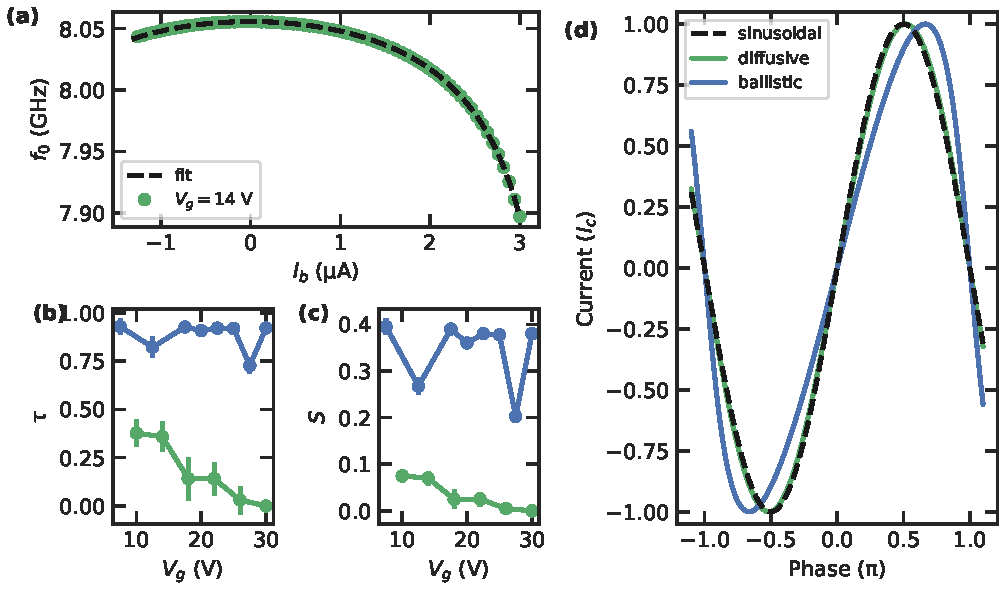
\includegraphics[width=\linewidth]{chapter-gJJ-CPR/figs/Figure5}
	\caption{
		\textbf{Extracting the current phase relation from current-biasing the gJJ microwave circuit.}
		%
		Fitting the bias current dependence \textbf{(a)}, we can extract the junction transparency \textbf{(b)} and corresponding CPR skew \textbf{(c)} for the diffusive (green) and ballistic (blue) gJJ device versus gate voltage.
		%
		\textbf{(d)} Reconstructed current-phase relation for the diffusive (green) and ballistic (blue) device.
		%
		The large transparency of the ballistic JJ leads to significant forward skewing, while the relatively low transparency of the diffusive JJ only results in minor skewing.
	}
	\label{fig:figure5}
\end{figure}

\section{Conclusion}

The influence of high microwave powers on the CPR: Bias current dependence as we shake the washboard a lot

Use a SQUID to measure the CPR in-situ: full circle

gJJ seem unfeasible for high-power cQED applications such as quantum-limited parametric amplification due to the intrinsic circuit losses.
%
Nevertheless, their application in lower power circuits, such as transmon qubits, should be investigated further.

%%%%%%%%%%%%%%%%%%%%%%%%%%%%%%%%%%%
% Insert SM.tex contents here

\pagebreak
\clearpage
%\widetext

%\setcounter{equation}{0}
%\setcounter{figure}{0}
%\setcounter{table}{0}
%\setcounter{page}{1}
%\setcounter{section}{0}

%\renewcommand{\thepage}{S\arabic{page}}
%\renewcommand{\thesection}{S\Roman{section}}
%\renewcommand{\thetable}{S\Roman{table}}
%\renewcommand{\thefigure}{S\arabic{figure}}
%\renewcommand{\theequation}{S\arabic{equation}}
%\renewcommand{\bibnumfmt}[1]{[S#1]}
%\renewcommand{\citenumfont}[1]{S#1}

\section{Supplementary Material: Current phase relations of graphene Josephson junctions in microwave circuits}

\subsection{Circuit parameters}

\begin{table}
	\centering
	\caption{\textbf{Circuit parameters as extracted for the various measurements}}
	\begin{tabular}{cccc}
		\hline\hline
		& Diffusive JJ & \multicolumn{2}{c}{Ballistic JJ}  \\
		Temperature & \SI{15}{\milli\kelvin} & \SI{15}{\milli\kelvin} & \SI{1}{\kelvin} \\
		\hline
		$f_{\lambda/2}$ (\si{\giga\hertz}) & $1.23\pm0.22$ & $1.23\pm0.22$ & $1.23\pm0.22$ \\
		$L_r$ (\si{\nano\henry}) & $1.23\pm0.22$ & $1.23\pm0.22$ & $1.23\pm0.22$ \\
		\hline\hline
	\end{tabular}
	\label{tab:frLr}
\end{table}

\begin{table}
	\centering
	\caption{\textbf{Circuit parameters as extracted for the various measurements}}
	\begin{tabular}{cccccc}
		\hline\hline
		& \multicolumn{2}{c}{Diffusive JJ} & \multicolumn{3}{c}{Ballistic JJ}  \\
		Temperature & \multicolumn{2}{c}{\SI{15}{\milli\kelvin}} & \multicolumn{2}{c}{\SI{15}{\milli\kelvin}} & \SI{1}{\kelvin} \\
		Measurement type & $I_b=0$ & $I_b\neq 0$ & $I_b=0$ & $I_b\neq 0$ & $I_b=0$ \\
		\hline
		$f_{\lambda/2}$ (\si{\giga\hertz}) & $1.23\pm0.22$ & $1.23\pm0.22$ & $1.23\pm0.22$ & $1.23\pm0.22$ & $1.23\pm0.22$ \\
		$L_r$ (\si{\nano\henry}) & $1.23\pm0.22$ & $1.23\pm0.22$ & $1.23\pm0.22$ & $1.23\pm0.22$ & $1.23\pm0.22$ \\
		\hline\hline
	\end{tabular}
	\label{tab:frLr2}
\end{table}

\subsection{Extraction of $I_s^{\rm DC}$ and $f_0$}\label{sec:extraction}

The DC switching current (Fig.~\ref{fig:figure1}(b,c)) is taken as the current at which $\partial V/\partial I_b$ is maximum, where $V$ is the measured voltage.
%
Noise or interference on the DC lines could lead to a reduction of the measured $I_s$ compared to the true $I_c$.
%
To get a more accurate estimation of $I_c$ together with a good understanding of the noise sources, switching histograms are the preferred measurement method.
%
The necessary setup was however not available at the time of measurement.

To extract resonance frequency and loss rates from the RF data, we fit the reflection coefficient to the following model (cf. Ref.~\cite{bosmanBroadbandArchitectureGalvanically2015c} for a derivation):
%
\begin{align}
S_{11}(\omega) = -1+\frac{2\kappa_e}{\kappa+2i\Delta},
\end{align}
%
where $\kappa=\kappa_e+\kappa_i$ denoting the total, external and internal loss rates, respectively, and $\Delta=\omega-\omega_0$ with resonance frequency $\omega_0=2\pi f_0$.
%
The measured $S_{11}$ is usually distorted by a setup-related microwave background of the following shape:
\begin{align}
B(\omega) = \left(a+b\omega+c\omega^2\right)e^{i\left(a^\prime+b^\prime\omega\right)},
\end{align}
%
and with additional rotation by angle $\theta$ in the complex plane, the measured $S_{11}^\prime$ is:
\begin{align}
S_{11}^\prime(\omega)=B(\omega)\left(e^{i\theta}\left(S_{11}(\omega)+1\right)-1\right)
\end{align}
%
The origin of the microwave background and phase rotations are impedance mismatches in the wiring originating from various non-ideal circuit elements (e.g. connectors, attenuators, directional couplers).
%
Standing waves can form in some segments of the wiring which interfere with the measured signal.

For the gate voltage sweeps (Fig.~\ref{fig:figure1}(d,e)), we pick the measurement trace at the CNP as the one with only background signal, as the RF resonance is extremely broad and effectively not present anymore.
%
We then divide the other traces by this background, resulting in a much cleaner signal.

For measurements based on bias current sweeps, cf. Fig~\ref{fig:figure5}(a), we take the RF background at $I_b>I_s$ at which the JJ switched to the normal state and the RF resonance is removed from the measurement and divide it off the cases at which there is a circuit resonance.

In order to remove RF background from the power dependence, we mask the regions in which there are resonances for the various powers and gate voltage setpoints, and average the remaining traces.
%
This way, we obtain a power and frequency map of the RF background, which we use for removing background signal from power traces, such as the one in Fig.~\ref{fig:figure4}(a).

\subsection{Derivation and validity of Eq.~\ref{eq:Pogorzalek}}\label{sec:validity}

\begin{figure}
	\centering
	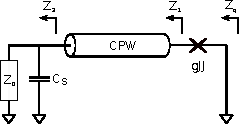
\includegraphics[width=0.5\linewidth]{chapter-gJJ-CPR/figs/rfderivation}
	\caption{
		\textbf{Derivation of resonance frequency.}
		%
		We define the three impedances $Z_1$, $Z_2$ and $Z_q$ as seen from the CPW towards the input port, from the gJJ towards the CPW, and as the parallel circuit impedance.
	}
	\label{fig:rfderivation}
\end{figure}

We can derive an expression for the circuit resonance frequency depending on the other parameters by using the impedances defined in Fig.~\ref{fig:rfderivation}.
%
The circuit impedance as seen from the JJ towards the CPW, $Z_1$, the input impedance as seen from the CPW towards the input port, $Z_2$, and the overall parallel circuit impedance $Z_q$ are defined as follows:
%
\begin{align}
Z_1 &= Z_0 \frac{Z_2+Z_0\tanh\gamma l}{Z_0+Z_2\tanh\gamma l} \\
Z_2 &= \left(\frac{1}{Z_{C_s}}+\frac{1}{Z_0}\right)^{-1} = \left(i\omega C_s+\frac{1}{Z_0}\right)^{-1} \\
Z_q &= \left(\frac{1}{Z_{JJ}}+\frac{1}{Z_1}\right)^{-1} = \left(\frac{1}{i\omega L_J}+\frac{1}{Z_1}\right)^{-1}\ ,
\end{align}
%
with the CPW length $l$, the complex CPW loss per unit length $\gamma=\alpha+i\beta$, and the transmission line impedance $Z_0$.
%
Assuming negligible losses in the CPW, $\gamma l\approx i\beta l = i\pi\omega_0/\omega_r$ (i.e. the CPW only acts as a phase shifter) on resonance.
%
Using $\tanh(iz)=i\tan(z)$, the resonance condition of the above circuit is for the imaginary part of the admittance $Y=1/Z_q=0$, which yields
%
\begin{align}
0 = \Im \left[ \frac{1}{i\omega_0 L_J} + \frac{1}{Z_0}\frac{Z_0+iZ_2\tan\left(\pi\omega_0/\omega_r\right)}{Z_2+iZ_0\tan\left(\pi\omega_0/\omega_r\right)}\right]
\label{eq:SolAnalytical}
\end{align}
%
The solution of this equation for $\omega_0$ is plotted as solid line in Fig.~\ref{fig:SMval}(a).
%
We can approximate the above by a similar method as the authors of Refs.~\cite{wallquistSelectiveCouplingSuperconducting2006a,wustmannParametricResonanceTunable2013,pogorzalekHystereticFluxResponse2017}:
%
Assuming $Z_2\approx 0$ and expanding the tangent, we arrive at the expression stated in Eq.~\ref{eq:Pogorzalek} which is plotted as dashed line in Fig.~\ref{fig:SMval}(a).
%
We find that for all values of $L_J$, including the range in our experiments, the approximation differs by no more than \SI{1}{\percent} from the analytical solution, regardless of JJ to CPW impedance, cf. Figs.~\ref{fig:SMval}(b-c).


\begin{figure}
	\centering
	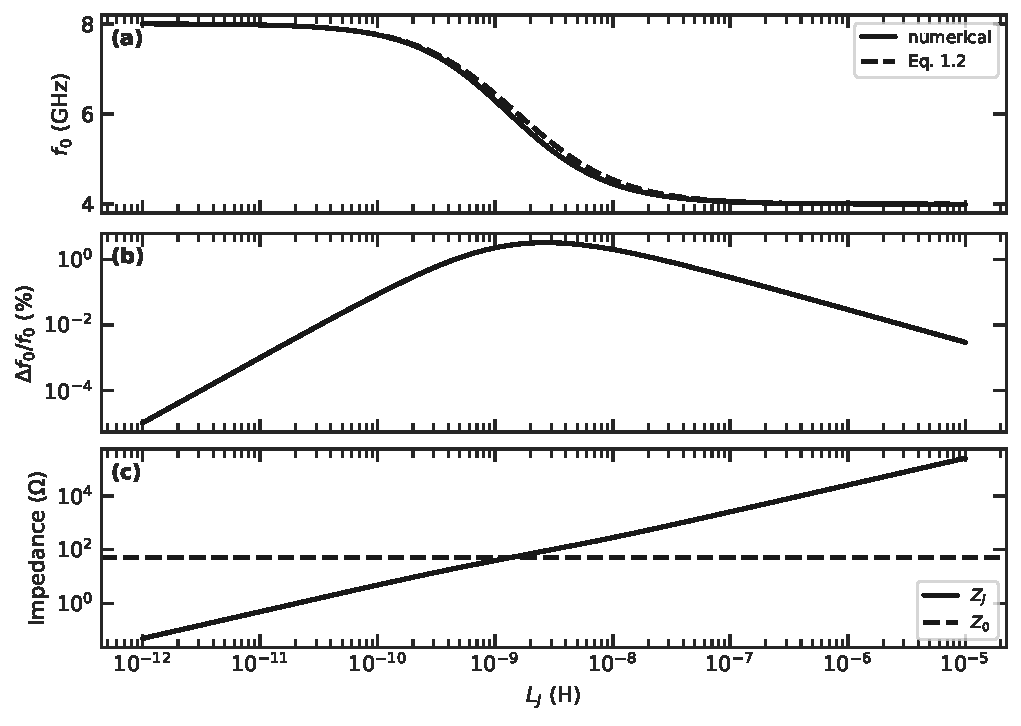
\includegraphics[width=0.5\linewidth]{chapter-gJJ-CPR/figs/SMFigure-validity}
	\caption{
		\textbf{Validity of Eq.~\ref{eq:Pogorzalek}.}
		%
		The equation used for modeling $f_0$ of the microwave circuit is an approximation to the true value.
		%
		\textbf{(a)} Resonance frequency as calculated using the  (solid) and using Eq.~\ref{eq:Pogorzalek} (dashed) for increasing Josephson inductance.
		\textbf{(b)} Relative difference between the two resonance frequencies.
		%
		\textbf{(c)} Impedance of the JJ (solid) and CPW impedance (dashed).
		%
		The approximation is in acceptable agreement with the full model regardless of $Z_J/Z_0$.
	}
	\label{fig:SMval}
\end{figure}


\subsection{Fitting procedure for extracting $\beta$}

Following the method described in Ref.~\cite{schmidtCurrentDetectionUsing2020}, the equation of motion of the amplitude field $\alpha(t)$ of a resonator with weak anharmonicity $\beta$ written in the frame rotating with the drive $S_{\rm in}$ is given by
%
\begin{align}
\dot{\alpha} = \left[ -i \left( \Delta+\beta\abs{\alpha}^2 \right)-\frac{\kappa}{2} \right]\alpha + \sqrt{\kappa_\text{e}} S_\text{in}\ ,
\label{eq:Duffing-EOM}
\end{align}
%
from which the steady-state solution $\dot{\alpha_0}=0$ results in the following polynomial function,
% 
\begin{align}
\beta^2 \alpha_0^6 + 2\Delta\beta\alpha_0^4 + \left(\Delta^2+\frac{\kappa^2}{4}\right)\alpha_0^2 - \kappa_\text{e} \abs{S_{\rm in}}^2 = 0\ ,
\label{eq:polynom}
\end{align}
%
which we can solve numerically and use to calculate the expected reflection coefficient,
\begin{align}
S_{11}=-1-\frac{\sqrt{\kappa_e}}{S_{\rm in}}\alpha_0\ .
\label{eq:S11anh}
\end{align}
%
We reduce the number of free parameters from five to two by fixing $\omega_0$ and $\kappa_e$ as the values extracted at lowest drive power and calculating $S_{\rm in}$ from the fridge attenuation, see Supplementary Section Sec.~\ref{sec:attenuation}.
%
The remaining parameters are $\beta$ and $\kappa_i$, where the internal loss rate can in fact depend on the drive power, $\kappa_i=\kappa_i(S_{\rm in})$.
%
Our algorithm first fits the measured data to return constant $\beta$ and $\kappa_i$, and uses these as initial values for a fit to extract the power dependent loss rate, shown in Fig.~\ref{fig:SMFig-lossrates}.

\subsection{Fitting procedure for extracting $\tau$}

\begin{figure}
	\centering
	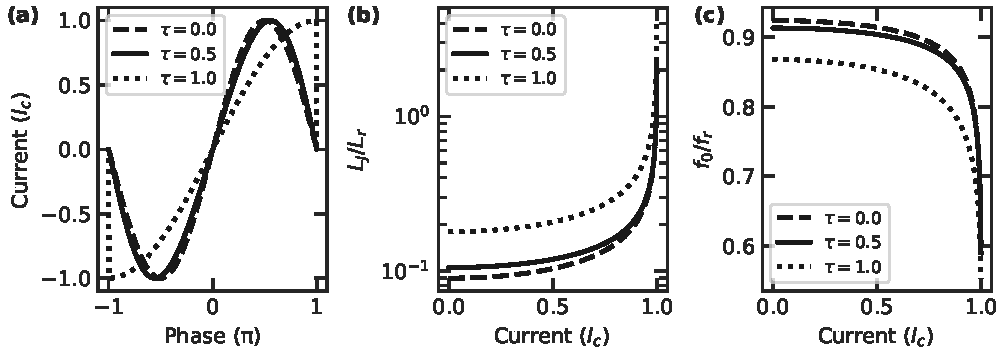
\includegraphics[width=\linewidth]{chapter-gJJ-CPR/figs/SMFigure-influence}
	\caption{
		\textbf{Predicted influence of the junction transparency on the bias current dependence.}
		%
		\textbf{(a)} CPR for various $\tau=0$ (solid), $\tau=0.5$ (dashed) and $\tau=1.0$	(dash-dotted).
		%
		\textbf{(b-c)} Josephson inductance \textbf{(b)} and resonance frequency \textbf{(c)} supercurrent for	same transparencies as in \textbf{(a)}.
		%
		Increased junction transmission leads to forward skewing of the CPR, thus a reduced slope and higher Josephson inductance, which in turn reduces the resonance frequency and increases the tuning.
	}
	\label{fig:SMinfluence}
\end{figure}

Without any knowledge on the junction transparency $\tau$, fitting data of a CPW cavity with JJ exhibiting a potentially nonsinusoidal CPR can lead to significant deviations from the true circuit parameters.
%
In Fig.~\ref{fig:SMtau}, we demonstrate the effect of $\tau$ on the extracted circuit parameters:
%
If the JJ shorting the CPW to ground has a forward skewed CPR, i.e. $\tau>0$, and Eq.~\ref{eq:Pogorzalek} is used to fit this data (dashed lines in Fig.~\ref{fig:SMtau}) under the assumption of a JJ with purely sinusoidal CPR, the extracted values (solid lines) for $f_r$ and $L_r$ will be too small compared with the true values, while $I_c$ will appear to be larger than expected, with consequently lower $L_J$.
%
Naively, one would assume the RF measurement to result in $L_J$ to be larger than the value expected from DC measurements due to the increased inverse CPR slope for identical $I_c$.
%
Nonetheless, the fit model accounting for the resonator tunability results in the opposite behavior.

To fit the bias current dependence data for extracting $\tau$, we first keep $\tau$ fixed and compare the fit residuals for various $\tau\in[0,1]$, cf. Fig.~\ref{fig:SMres}(a).
%
In a second step, we set $\tau$ as additional free parameter with the best results for $f_r$, $L_r$ and $I_c$, and set the initial value of $\tau$ as the one with previously determined minimum reduced $\chi^2$.
%
The fit converges more reliably than by setting $\tau$ as free parameter from the start, since this way the fit does not get trapped in a local minima.

Both current and frequency noise, however, can result in artificial global minima in $\chi^2(\tau)$, as shown in Fig.~\ref{fig:SMres}(b-c).
%
For a critical current of \SI{2}{\micro\ampere} and bias currents up to $0.9I_c$, already $\sigma_I\geq\SI{1}{\nano\ampere}$ is enough to significantly throw off the fit for low values of $\tau$.
%
Frequency noise of $\sigma_f<\SI{1}{\mega\hertz}$ has no influence on the fitting algorithm.
%
As the responsivity $\partial f_0/\partial I_b$ increases with $I_b$, so does the frequency noise for a fixed current noise, cf. Fig.~\ref{fig:SMres}(d).
%
From the average data fluctuations and comparing these with the expected $\sigma_f(\sigma_I)$, we estimate $\sigma_I<\SI{1}{\nano\ampere}$ in our setup.
%
We therefore conclude that our fitting algorithm should present a reliable way of extracting $\tau$. 

\begin{figure}
	\centering
	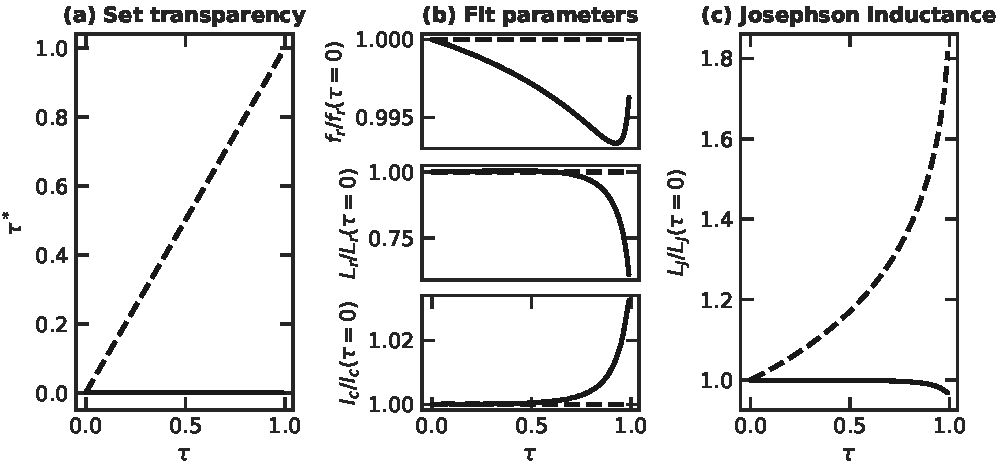
\includegraphics[width=\linewidth]{chapter-gJJ-CPR/figs/SMFigure-tauparams}
	\caption{
		\textbf{Influence of $\tau$ on extracted fit parameters with Eq.~\ref{eq:Pogorzalek}.}
		Increasing $\tau$ (dashed line in \textbf{(a)}) results in a larger $L_J$ (dashed line in \textbf{(e)}), while the other fit parameters (dashed lines in \textbf{(b-d)}) remain constant.
		%
		In order for a fit model using Eq.~\ref{eq:Pogorzalek} under the assumption of a sinusoidal CPR (solid lines) to reproduce the data (points), significant deviations from the true parameters occur.
		%
		Specifically, the fit model returns a larger critical current than expected which leads to a reduced calculated $L_J$, even though the real $L_J$ increases with $\tau$.
	}
	\label{fig:SMtau}
\end{figure}

\begin{figure}
	\centering
	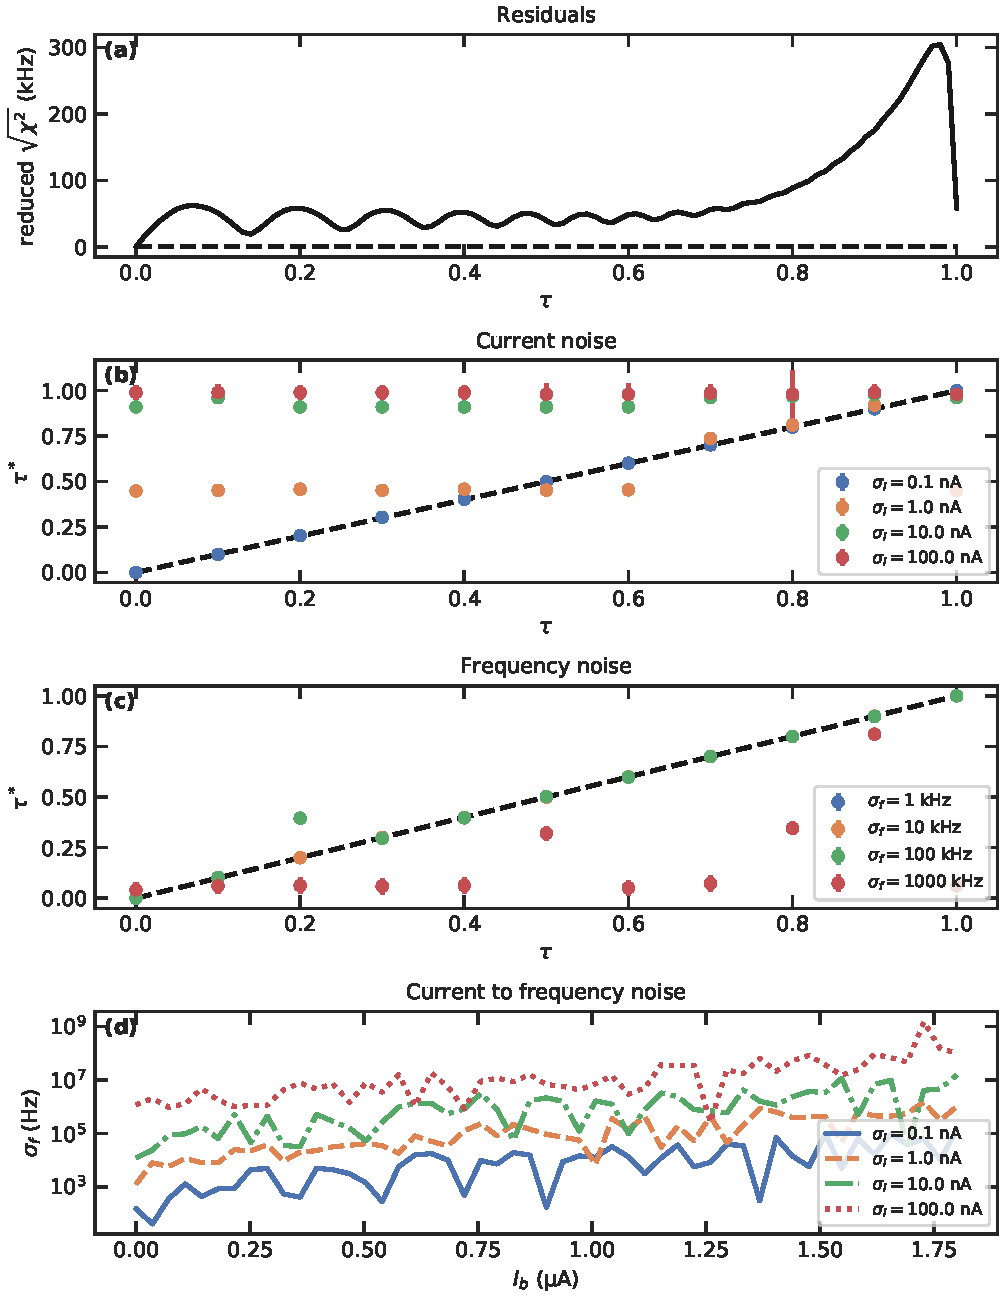
\includegraphics[width=\linewidth]{chapter-gJJ-CPR/figs/SMFigure-noise}
	\caption{
		\textbf{Influence of $\tau$ and noise on fit result.}
		\textbf{(a)} Assuming a sinusoidal CPR for Eq.~\ref{eq:Pogorzalek} to fit data originating from a forward skewed CPR results in minimum fit residuals for $\tau=0$ (solid line).
		%
		Assuming the correct $\tau$ however results in minimum residuals (dashed line).
		%
		\textbf{(b-d)} Both current and frequency noise can significantly throw off the fitting algorithm by creating artificially global residual minima.
		%
		Plotted are calculations for $I_c=\SI{2}{\micro\ampere}$.
		%
		We estimate $\sigma_I<\SI{1}{\nano\ampere}$ in our setup.
	}
	\label{fig:SMres}
\end{figure}

\subsection{Internal loss rate dependence on gate voltage, bias current and drive power}\label{sec:kintib}

The internal loss rate of our circuit depends on various parameters.

\begin{itemize}
	\item \textbf{Gate voltage dependence, cf. Fig~\ref{fig:SMFig-lossrates}(a)}
	\item \textbf{Bias current dependence, cf. Fig~\ref{fig:SMFig-lossrates}(b)}
	\item \textbf{Drive power dependence, cf. Fig~\ref{fig:SMFig-lossrates}(c)}
\end{itemize}

\begin{figure}
	\centering
	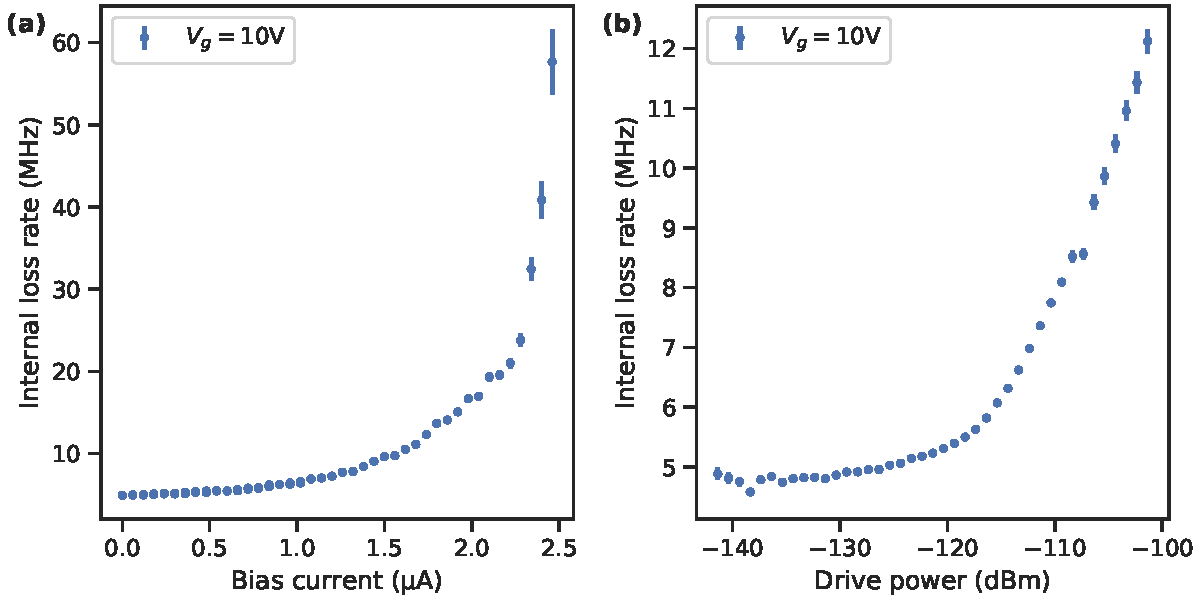
\includegraphics[width=0.583\linewidth]{chapter-gJJ-CPR/figs/SMFigure-lossrates}
	\caption{
		\textbf{Internal loss rate for varying gate voltage (a), increasing bias current (b) and drive power (c).}
		%
		Higher losses around the CNP and for $V_g<0$ are presumably due to a higher number of subgap states.
		%
		Increasing loss rate with bias current could originate from either low-frequency noise or phase slip events.
		%
		An increase in $\kappa_i$ with drive power could be due to subgap states in the gJJ.
	}
	\label{fig:SMFig-lossrates}
\end{figure}


\subsection{Estimation of the fridge attenuation}\label{sec:attenuation}
The HEMT noise power is given by
%
\begin{align}
P_{\rm HEMT}=10\log\left(\frac{k_B T_{\rm HEMT}}{\si{\milli\watt}}\right) + 10\log\left(\frac{\Delta f}{\si{\hertz}}\right)\ ,
\label{eq:HEMT}
\end{align}
%
with the Boltzmann constant $k_B$, the noise temperature of the HEMT $T_{\rm HEMT}=\SI{2}{\kelvin}$ as specified by the manufacturer and the measurement bandwidth $\Delta f=\SI{100}{\hertz}$ resulting in $P_{\rm HEMT}\approx\SI{-175.59}{dBm}$.

By averaging over a few $S_{11}$ traces taken with the VNA in an area unaffected by our DUT, i.e. off-resonant to the cavity and thus leaving the background unaltered in power, we extract an average signal and standard deviation which we use to define the signal-to-noise ratio at the VNA, $\text{SNR}_\text{VNA}=\SI{34.5}{\decibel}$ for a VNA output power of \SI{0}{dBm}.

attenuation of \SI{129.3}{dB} of our VNA input line, assuming $X=\SI{2}{dB}$ of cable loss between sample and HEMT

\references{dissertation}


%\newchapstyle
\chapter{Current detection using a Josephson parametric upconverter}
\label{chap:currentdetection}

%% The following annotation is customary for chapter which have already been
%% published as a paper.
\blfootnote{
	\color{title}
	A preprint of this chapter is available at arXiv:2001.02521~\cite{schmidtCurrentDetectionUsing2020}.
	%
	Data and code to reproduce the calculations and figures presented here can be found on Zenodo~\cite{schmidtDataProcessingCurrent2020}.
}

\begin{abstract}
	
	We present the design, measurement and analysis of a current sensor based on a process of Josephson parametric upconversion in a superconducting microwave cavity. 
	%
	Terminating a coplanar waveguide with a nanobridge constriction Josephson junction, we observe modulation sidebands from the cavity that enable highly sensitive, frequency-multiplexed output of small currents for applications such as transition-edge sensor array readout. 
	%
	We derive an analytical model to reproduce the measurements over a wide range of bias currents, detunings and input powers.
	% 
	Tuning the frequency of the cavity by more than \SI{100}{\mega\hertz} with DC current, our device achieves a minimum current sensitivity of \SI{8.9}{\pico\ampere\per\hertz\tothe{1/2}}.
	% 
	Extrapolating the results of our analytical model, we predict an improved device based on our platform, capable of achieving sensitivities down to \SI{50}{\femto\ampere\per\hertz\tothe{1/2}}, or even lower if one could take advantage of parametric amplification in the Josephson cavity.
	% 
	Taking advantage of the Josephson architecture, our approach can provide higher sensitivity than kinetic inductance designs, and potentially enables detection of currents ultimately limited by quantum noise.
\end{abstract}

%%%%%%%%%%%%%%%%%%%%%%%%%%%%%%%%%%%%%%%%%%%%%%%%%%%%%%%%%%%%%%%%%%%%%%%%%%%%%%%%%%%%%%%%%%%%%%%%%%%%%%%%%%%%%%%%%%%%%%%%%
%%%%%%%%%%%%%%%%%%%%%%%%%%%%%%%%%%%%%%%%%%%%%%%%%%%%%%%%%%%%%%%%%%%%%%%%%%%%%%%%%%%%%%%%%%%%%%%%%%%%%%%%%%%%%%%%%%%%%%%%%
%%%%%%%%%%%%%%%%%%%%%%%%%%%%%%%%%%%%%%%%%%%%%%%%%%%%%%%%%%%%%%%%%%%%%%%%%%%%%%%%%%%%%%%%%%%%%%%%%%%%%%%%%%%%%%%%%%%%%%%%%
%%%%%%%%%%%%%%%%%%%%%%%%%%%%%%%%%%%%%%%%%%%%%%%%%%%%%%%%%%%%%%%%%%%%%%%%%%%%%%%%%%%%%%%%%%%%%%%%%%%%%%%%%%%%%%%%%%%%%%%%%
\afterpage{\pagecolor{none}}\newpage
\section{Introduction}

Ultra-low noise radiation detection has applications in astronomy, particle physics, and quantum information processing.
% 
In particular, transition edge sensors (TES) allow for broadband radiation detection with exceptionally low noise equivalent power~\cite{goldieUltralownoiseMoCuTransition2011} and photon number resolution~\cite{cabreraDetectionSingleInfrared1998,millerDemonstrationLownoiseNearinfrared2003}.
% 
To read out the small changes in current of TES in response to radiation absorption, highly sensitive current amplifiers such as superconducting quantum interference devices (SQUIDs) can be used with sensitivities as low as \SI{4}{\femto\ampere\per\hertz\tothe{1/2}}~\cite{gayUltralowNoiseCurrent2000}.
% 
However, with the increasing number of TES to be read out simultaneously in multipixel detectors, SQUID amplifiers significantly increase system cost and complexity, especially when employing frequency-domain multiplexing to reduce the number of necessary amplifiers~\cite{hendersonReadoutTwokilopixelTransitionedge2016}.

An example of recently developed current detectors as a replacement of SQUIDs are kinetic inductance parametric upconverters (KPUPs), also referred to as microwave kinetic inductance nanowire galvanometers, which rely on the changing kinetic inductance $L_\text{k}$ of a narrow superconducting wire embedded in a microwave circuit in response to a DC bias current, with state of the art devices reaching current sensitivities $\mathcal{S}_I$ between \SIrange{5}{10}{\pico\ampere\per\hertz\tothe{1/2}}~\cite{kherKineticInductanceParametric2016,doernerCompactMicrowaveKinetic2018,kuzminTerahertzTransitionEdgeSensor2018}.
%
One could potentially achieve a higher response from such a cavity detector by replacing the nanowire kinetic inductance element with a Josephson junction (JJ), enabling detection of currents using a Jospheson parametric upconverter (JPUP). 
% 
This would also enable the incorporation of processes such as Josephson parametric amplification, which allows signals to be amplfied with quantum limited noise~\cite{stehlikFastChargeSensing2015}, directly in the readout cavity.

Typically, the integration of JJs in superconducting microwave circuits is technologically more demanding due to the additionally needed fabrication steps to avoid aging effects and low coherence at microwave frequencies~\cite{pavolotskyAgingAnnealinginducedVariations2011,gotetiReliabilityStudiesNb2019,gunnarssonDielectricLossesMultilayer2013,yanaiObservationEnhancedCoherence2019}.
% 
The intrinsically large Kerr-nonlinearity of JJs~\cite{wallraffStrongCouplingSingle2004e} can additionally place an upper limit on the device power allowed for circuit operation, which calls for either large critical current JJs with additional fabrication challenges~\cite{lecocqJunctionFabricationShadow2011b}, or appropriate circuit design for sufficiently diluting the nonlinearity to provide stable device operation.

Here, we provide experimental realisation of a JPUP based on a hybrid combination of a direct current (DC) accessible microwave cavity in coplanar waveguide (CPW) geometry~\cite{bosmanBroadbandArchitectureGalvanically2015c,schmidtBallisticGrapheneSuperconducting2018}.
% 
The design uses a constriction JJ fabricated in the same step and layer as the microwave cavity which simplifies the fabrication procedure and allows for high cavity drive powers~\cite{vijayOptimizingAnharmonicityNanoscale2009,kennedyTunableNbSuperconducting2019,rodriguesCouplingMicrowavePhotons2019,bothnerPhotonPressureStrongCouplingTwo2019}.
% 
We show device operation by converting \si{\kilo\hertz} current signals to the \si{\giga\hertz} range, and reproduce the data with an analytical model for a wide range of bias currents, drive detunings and drive powers.
%
Our device achieves performance comparable to KPUP technology, with the potential to provide enhanced current sensitivity with a more optimized design. Ultimately, by using Josephson parametric amplification in the same cavity as used for sensing, the JPUP could sense low frequency currents with a sensitivity limited by quantum noise.

%%%%%%%%%%%%%%%%%%%%%%%%%%%%%%%%%%%%%%%%%%%%%%%%%%%%%%%%%%%%%%%%%%%%%%%%%%%%%%%%%%%%%%%%%%%%%%%%%%%%%%%%%%%%%%%%%%%%%%%%%
%%%%%%%%%%%%%%%%%%%%%%%%%%%%%%%%%%%%%%%%%%%%%%%%%%%%%%%%%%%%%%%%%%%%%%%%%%%%%%%%%%%%%%%%%%%%%%%%%%%%%%%%%%%%%%%%%%%%%%%%%
%%%%%%%%%%%%%%%%%%%%%%%%%%%%%%%%%%%%%%%%%%%%%%%%%%%%%%%%%%%%%%%%%%%%%%%%%%%%%%%%%%%%%%%%%%%%%%%%%%%%%%%%%%%%%%%%%%%%%%%%%
%%%%%%%%%%%%%%%%%%%%%%%%%%%%%%%%%%%%%%%%%%%%%%%%%%%%%%%%%%%%%%%%%%%%%%%%%%%%%%%%%%%%%%%%%%%%%%%%%%%%%%%%%%%%%%%%%%%%%%%%%

\begin{figure*}[t]
	\centering
	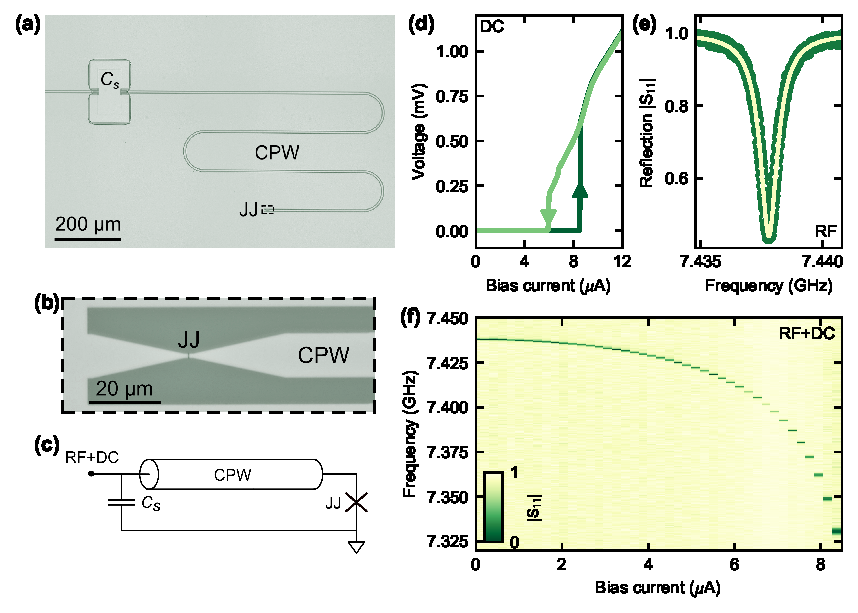
\includegraphics[width=\linewidth]{chapter-currentdetection/figures/Figure1}
	\caption{
		\textbf{A coplanar microwave Josephson circuit with direct current bias.}
		%
		(a) Optical image of the measured device.
		%
		It consists of a coplanar waveguide transmission line shunted to ground via a parallel plate capacitor $C_\text{s}$ on the input, and the Josephson junction shorting the CPW center conductor to ground on the far end.
		%
		(b) Optical close-up of the area around the JJ.
		%
		(c) Schematic circuit layout.
		%
		(d) Current-voltage characteristics of the JJ, measured by sweeping the bias current up and down (sweep direction indicated by arrows).
		%
		(e) Normalized and background-corrected reflection $\abs{S_{11}}$ of the device with zero bias current applied, cf. Sec.~\ref{sec:general-S11} of the Supplemental Material~\cite{SeeSupplementalMaterial}.
		%
		Circles: data, line: fit.
		%
		(f) Reflection coefficient $\abs{S_{11}}$ as a function of bias current.
		%
		Since the Josephson inductance increases with bias current, the resonance frequency of the circuit shifts towards lower values.
		%
		\label{fig:figure1}
	}
\end{figure*}

\section{The DC bias microwave circuit}

The device consists of a galvanically accessible microwave cavity, formed by a CPW that is shunted by an input capacitor $C_\text{s}$ and shorted to ground at its far end by a JJ, as depicted in Figs.~\ref{fig:figure1}(a-c).
% 
The JJ is formed by a narrow constriction in the superconducting base-layer, which allows us to fabricate it in the same step as the microwave circuit.
% 
For details on the fabrication procedure, see Sec.~\ref{sec:fabrication} of the Supplemental Material~\cite{SeeSupplementalMaterial}.
% 
Due to the shunt capacitor allowing low-frequency signals to pass through, but acting as a semi-transparent mirror for microwave frequencies, our circuit allows for simultaneous measurements in the DC and RF regimes.

% 
In the DC regime, the CPW center conductor acts as a long lead to the JJ, which we use to perform a current-voltage measurement to characterize the JJ.
% 
Upon applying an increasing DC bias current, the JJ switches from the superconducting to the voltage state and back again at switching and retrapping currents $I_\text{s}\approx\SI{8.5}{\micro\ampere}$ and $I_\text{r}\approx\SI{6.1}{\micro\ampere}$, as shown in Fig.~\ref{fig:figure1}(d).
% 
The observed hysteresis is most likely a combination of the capacitances of the CPW and shunt capacitor, and local heating in the junction area, cf. Refs.~\cite{tinkhamIntroductionSuperconductivity1996,skocpolSelfHeatingHotspots1974,hazraHysteresisSuperconductingShort2010,kumarReversibilitySuperconductingNb2015} and Sec.~\ref{sec:hysteresis} in the Supplemental Material~\cite{SeeSupplementalMaterial}.

In the RF regime, the JJ acts as a nonlinear inductor, with its inductance $L_\text{J}$ depending on the amount of bias current $I_\text{b}$ flowing through it, according to
% 
\begin{align}
L_\text{J}(I_\text{b})= \frac{\Phi_0}{2\pi \sqrt{I_\text{c}^2-I_\text{b}^2}}\ ,
\label{eq:Lj-of-I}
\end{align}
% 
with $I_\text{c}$ the critical current and $\Phi_0$ the magnetic flux quantum.
% 
For zero bias current, both the impedance of shunt capacitor and of the JJ are small compared to the characteristic impedance of the CPW, i.e. $\omega L_\text{J},1/\omega C_\text{s} \ll Z_0$.
% 
The CPW can thus host a fundamental half-wavelength ($\lambda/2$) mode with current antinodes at both ends.
% 
When recording the reflected signal of the device using single-tone RF spectroscopy, the reflection signal shows a dip in the spectrum as seen in Fig.~\ref{fig:figure1}(e).
% 
We fit the data using the reflection coefficient of our circuit,
% 
\begin{align}
S_{11} = \frac{\kappa_\text{e}-\kappa_\text{i}-2i\Delta}{\kappa_\text{e}+\kappa_\text{i}+2i\Delta}\ ,
\label{eq:general:S11}
\end{align}
% 
with $\Delta=\omega-\omega_0$ the detuning between a drive at $\omega$ and the resonance frequency $\omega_0$ and the external and internal loss rates $\kappa_\text{e}$ and $\kappa_\text{i}$, respectively~\cite{bosmanBroadbandArchitectureGalvanically2015c}.
% 
At zero bias current, we find a resonance frequency of $\omega_0=2\pi\times\SI{7.438}{\giga\hertz}$, and linewidths of $\kappa_\text{e}=2\pi\times\SI{624}{\kilo\hertz}$ and $\kappa_\text{i}=2\pi\times\SI{261}{\kilo\hertz}$.
%
Here, the external loss rate $\kappa_\text{e}$ describes how much signal leaks to the feedline, while $\kappa_\text{i}$ captures intracavity losses such as due to dielectrics or radiation, cf. Sec.~\ref{sec:general-S11} of the Supplemental Material.

% 
As we DC-bias the circuit, $L_\text{J}$ increases, effectively shifting the voltage antinode closer to the JJ.
% 
This results in a continuously decreasing resonance frequency, tuning over approximately \SI{108}{\mega\hertz}, cf. Fig.~\ref{fig:figure1}(f).
% 
We can approximate the bias current dependence of the cavity resonance frequency with a model describing a $\lambda/2$ CPW resonator terminated by a JJ via
% 
\begin{align}
\omega_0(I_\text{b})=\omega_{\lambda/2}\,\frac{L_\text{r} + L_\text{J}(I_\text{b},I_\text{c})}{L_\text{r} + 2L_\text{J}(I_\text{b},I_\text{c})}
\label{eq:f0vsI}
\end{align}
% 
with $\omega_{\lambda/2}$ the resonance frequency of the CPW directly shorted to ground and $L_\text{r}$ the total bare resonator inductance  (see Sec.~\ref{sec:resfit} of the Supplemental Material~\cite{SeeSupplementalMaterial} and Ref.~\cite{pogorzalekHystereticFluxResponse2017}).
% 
We use this model to fit the measured resonance frequencies in Fig.~\ref{fig:figure2}(a), from which we extract $\omega_{\lambda/2}=2\pi\times\SI{7.515}{\giga\hertz}$, $L_\text{r}=\SI{3.401}{\nano\henry}$ and $I_\text{c}=\SI{9.157}{\micro\ampere}$.
% 
The resonator inductance agrees with the value expected from our circuit design.
% 
The critical current as inferred from the microwave measurement is approximately \SI{8}{\percent} larger than the DC switching current.
% 
We suspect that current noise in the DC line leads to premature switching of the JJ in the IV measurements, resulting in $I_\text{s}<I_\text{c}$, as discussed in Sec.~\ref{sec:lossrates} of the Supplemental Material~\cite{SeeSupplementalMaterial} and Ref.~\cite{kautzNoiseaffectedIVCurves1990}.
% 
On the other hand, the RF measurement is sensitive to the Josephson inductance, from which we can infer the critical current in a less perturbative way.
% 
We note that current-biasing a superconducting wire will also change its kinetic inductance $L_\text{k}$~\cite{annunziataTunableSuperconductingNanoinductors2010b,vissersFrequencytunableSuperconductingResonators2015b}.
% 
However, while our device does possess a noticeable kinetic inductance fraction~\cite{gaoExperimentalStudyKinetic2006}, the changes in $L_\text{k}$ within the range of applied bias currents are negligible compared to $L_\text{J}$ and we thus attribute the resonance frequency shift completely to the latter, cf. Sec.~\ref{sec:Lk} of the Supplemental Material~\cite{SeeSupplementalMaterial}.

We note that upon increasing the DC bias current $I_\text{b}$, we observe an increase in internal loss rate $\kappa_\text{i}$ of our device.
%
We find that the dependence $\kappa_\text{i}(I_\text{b})$ can be approximated by a constant term and exponential growth, which we ascribe to a combination of low-frequency electrical interference of the DC bias current, and phase diffusion across the JJ, cf. Supplemental Material Sec.~\ref{sec:lossrates}.


%%%%%%%%%%%%%%%%%%%%%%%%%%%%%%%%%%%%%%%%%%%%%%%%%%%%%%%%%%%%%%%%%%%%%%%%%%%%%%%%%%%%%%%%%%%%%%%%%%%%%%%%%%%%%%%%%%%%%%%%%
%%%%%%%%%%%%%%%%%%%%%%%%%%%%%%%%%%%%%%%%%%%%%%%%%%%%%%%%%%%%%%%%%%%%%%%%%%%%%%%%%%%%%%%%%%%%%%%%%%%%%%%%%%%%%%%%%%%%%%%%%
%%%%%%%%%%%%%%%%%%%%%%%%%%%%%%%%%%%%%%%%%%%%%%%%%%%%%%%%%%%%%%%%%%%%%%%%%%%%%%%%%%%%%%%%%%%%%%%%%%%%%%%%%%%%%%%%%%%%%%%%%
%%%%%%%%%%%%%%%%%%%%%%%%%%%%%%%%%%%%%%%%%%%%%%%%%%%%%%%%%%%%%%%%%%%%%%%%%%%%%%%%%%%%%%%%%%%%%%%%%%%%%%%%%%%%%%%%%%%%%%%%%

\section{Current detection by frequency up-conversion}
% 
Figure~\ref{fig:figure2}(a) illustrates the principle of current detection using the DC biased Josephson cavity.
% 
To detect small modulation currents, we drive the cavity on resonance $\omega_0(I_\text{b})$ and simultaneously modulate the bias point $I_\text{b}$ with a low-frequency signal $\delta I=I_\text{LF}\cos{\Omega t}$, so that the total current is given by $I=I_\text{b}+I_\text{LF}\cos\Omega t$.
% 
The responsivity of the resonance frequency to bias current,
\begin{align}
G_1 = \frac{\partial\omega_0}{\partial I_\text{b}} \ ,
\end{align}
exceeds $2\pi\times\SI{100}{\mega\hertz\per\micro\ampere}$ for $I_\text{b}\gtrsim\SI{8}{\micro\ampere}$.
% 
As a consequence, once the resonance frequency is modulated by $I_\text{LF}$, phase modulation leads to the generation of sidebands in the microwave drive tone reflection with $\omega = \omega_\text{d} \pm n \Omega$, where $n \in \mathbb{Z}$.
% 
The reflected cavity field thus exhibits the drive tone together with the sidebands, as depicted in Fig.~\ref{fig:figure2}(b).

The general equation of motion for the amplitude field $\alpha$ of a harmonic high-$Q$ oscillator with small nonlinearity $\beta$, written in the frame rotating with the drive, is given by
% 
\begin{align}
\dot{\alpha} = \left[ -i \left( \Delta+\beta\abs{\alpha}^2 \right)-\frac{\kappa}{2} \right]\alpha + \sqrt{\kappa_\text{e}} S_\text{in}\ ,
\label{eq:Duffing-EOM}
\end{align}
% 
with $S_\text{in}$ the amplitude of the drive field in units of $\sqrt{\si{Photons\per\hertz}}$ at $\omega$, and $\beta$ a small nonlinearity~\cite{eichlerControllingDynamicRange2014d}.
% 
We consider the case in which the cavity resonance frequency is a function of an additional current given by $I = I_\text{b} + \delta I=I_\text{b}+I_\text{LF}\cos\Omega t$, such that
% 
\begin{align}
\begin{split}
\omega_0 &= \omega_0(I_\text{b}) + \sum_{m=1}^n \frac{\partial^m \omega_0}{\partial I^m}\delta I^m = \omega_I + \sum_{m=1}^n G_m \delta I^m \ .
\label{eq:omega_Taylor}
\end{split}
\end{align}
% 
The resulting field amplitude of the first order sidebands appearing at $\omega_0\pm1\Omega$ is
% 
\begin{align}
\abs{S_{\pm 1}}^2 = \frac{\kappa_\text{e}\alpha_0^2 G_1^2 I_\text{LF}^2}{\kappa^2+4(\Delta\pm\Omega)^2}\ .
\label{eq:first_amplitude}
\end{align}


\begin{figure}[t]
	\centering
	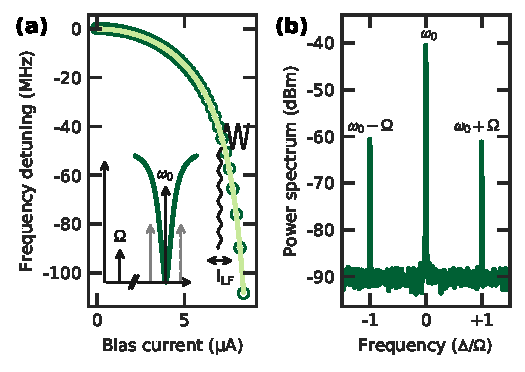
\includegraphics[width=.5\linewidth]{chapter-currentdetection/figures/Figure2}
	\caption{
		\textbf{Current detection by frequency up-conversion.}
		%
		(a) Cavity resonance frequency for increasing DC bias current, showing a total frequency shift of $\SI{108}{\mega\hertz}$.
		%
		Circles: measured data, line: fit to resonance frequency using Eq.\eqref{eq:f0vsI}.
		%
		Inset: sketched measurement scheme in the frequency domain.
		%
		By driving the cavity on resonance $\omega = \omega_0$ and simultaneously modulating with a low frequency current $\delta I = I_\text{LF}\cos\Omega t$, the cavity generates sidebands to the drive tone at $\omega_0 \pm \Omega$ (dashed grey arrows).
		%
		(b) The power spectrum of the reflected field at $I_\text{b}=\SI{2.5}{\micro\ampere}$, containing the input pump signal at $\omega_0$ and the first order sidebands due to mixing at $\omega_0 \pm \Omega$.
		%
		The noise floor sets a lower limit on the smallest detectable sideband amplitude.
		%
		The sideband amplitude allows us to directly calibrate the noise floor and thus the sensitivity from the signal-to-noise ratio, here $\text{SNR}\approx\SI{30}{\decibel}$.
		%
		\label{fig:figure2}
	}
\end{figure}


In our experiment, we chose $\Omega=2\pi\times\SI{1}{\kilo\hertz}$ and $I_\text{LF}=\SI{10}{\nano\ampere}$.
% 
In this case, $\Omega\ll\kappa$ and red ($S_{-}$) and blue ($S_{+}$) sidebands have approximately equal amplitudes, see Sec.~\ref{sec:bluered} of the Supplemental Material~\cite{SeeSupplementalMaterial}.
% 
Note that even higher order contributions from the current still contribute to the $\pm1\Omega$ sideband, but those contributions can be neglected for relatively weak modulation.



% \section{Parameter space exploration}
% 
To explore the parameter space of our device, we performed a series of current-mixing measurements for different values of bias current $I_\text{b}$, drive detuning $\Delta$ and drive amplitude $S_\text{in}$, for all of which we observe excellent agreement between experiment and theory:
% 
As can be seen in Fig.~\ref{fig:figure3}(a), for the case of varying bias current and as expected from Eqs.~\eqref{eq:f0vsI},\eqref{eq:first_amplitude}, the first order sideband vanishes for zero bias current.
% 
As we increase the DC bias current, the increasing Josephson inductance leads to an increased responsivity $\partial\omega_0/\partial I_\text{b}$, which in turn results in a growing sideband amplitude.
% 
Assuming all other parameters remain constant, the sideband amplitude should keep growing until the bias current reaches the critical current of the JJ, at which point the junction switches to the normal state, effectively destroying the device response.
% 
However, already at $I_\text{b} \approx 0.75 \,I_\text{c}$ the sideband amplitude exhibits a maximum value and begins to decrease subsequently.
% 
The origin for this phenomenon lies in the growth of $\kappa_\text{i}$ for increasing $I_\text{b}$ as described earlier, which limits the maximum achievable sideband amplitude, cf. Sec.~\ref{subsec:limitations} and Sec.~\ref{sec:lossrates} of the Supplemental Material~\cite{SeeSupplementalMaterial}.

Operating the device at constant bias current and drive power $P_\text{in}$ but sweeping the drive tone with respect to the cavity resonance similarly reduces the sideband amplitude, which is reflected in both the theoretical model and our measurements, cf. Fig.~\ref{fig:figure3}(b).
% 
We attribute deviations of the model from the data to an effectively increased cavity linewidth resulting from a noise-induced fluctuating cavity frequency.

Finally, when setting the detuning back to zero and sweeping the drive power, we initially observe a linear increase of the sideband amplitude, cf. Fig.~\ref{fig:figure3}(c).
% 
This is in good agreement with the intracavity field dependence with pump power of a linear cavity.
% 
However, due to the nonlinearity of the JJ and the resulting Kerr anharmonicity of the circuit, our device enters the Duffing regime for large input powers, resulting in the observable reduction of the sideband amplitude:
% 
The anharmonicity results in a down shifted resonance frequency given by $\omega_0' = \omega_0-\abs{\alpha_0}^2\beta$.
% 
In the measurement depicted in Fig.~\ref{fig:figure3}(c), the only varying parameter is the pump power, which means that in the Duffing regime the drive acquires an increase in detuning for increased power, resulting in a decreased sideband amplitude, as we saw earlier.

\begin{figure*}[]
	\centering
	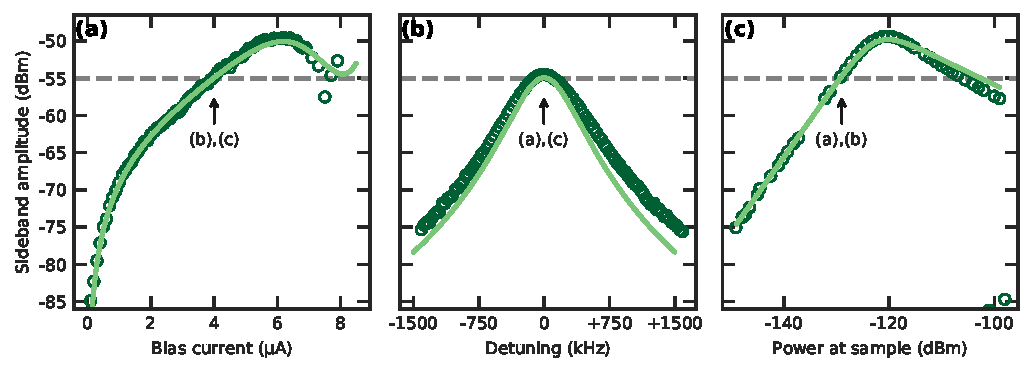
\includegraphics[width=\linewidth]{chapter-currentdetection/figures/Figure3}
	\caption{
		\textbf{Exploring the parameter space for the first order sideband amplitude.}
		% 
		(a) Sideband height for changing bias current setpoint at fixed input power and zero detuning. % approximately \SI{-129}{dBm}
		% 
		(b) Sideband height for changing drive detuning at fixed input power and bias current.
		% 
		(c) Sideband height for changing input power at fixed bias current and detuning. %\SI{4}{\micro\ampere}
		% 
		Circles: measured data, solid lines: calculated amplitude via input-output theory, dashed grey line: calculated sideband amplitude at $I_\text{b}=\SI{4}{\micro\ampere}$, $\Delta=0$ and $P_\text{in}=\SI{-129}{dBm}$.
		% 
		Arrows indicate the setpoints for the other respective panels.
		% 
		\label{fig:figure3}
	}
\end{figure*}

%%%%%%%%%%%%%%%%%%%%%%%%%%%%%%%%%%%%%%%%%%%%%%%%%%%%%%%%%%%%%%%%%%%%%%%%%%%%%%%%%%%%%%%%%%%%%%%%%%%%%%%%%%%%%%%%%%%%%%%%%
%%%%%%%%%%%%%%%%%%%%%%%%%%%%%%%%%%%%%%%%%%%%%%%%%%%%%%%%%%%%%%%%%%%%%%%%%%%%%%%%%%%%%%%%%%%%%%%%%%%%%%%%%%%%%%%%%%%%%%%%%
%%%%%%%%%%%%%%%%%%%%%%%%%%%%%%%%%%%%%%%%%%%%%%%%%%%%%%%%%%%%%%%%%%%%%%%%%%%%%%%%%%%%%%%%%%%%%%%%%%%%%%%%%%%%%%%%%%%%%%%%%
%%%%%%%%%%%%%%%%%%%%%%%%%%%%%%%%%%%%%%%%%%%%%%%%%%%%%%%%%%%%%%%%%%%%%%%%%%%%%%%%%%%%%%%%%%%%%%%%%%%%%%%%%%%%%%%%%%%%%%%%%
\section{Current sensitivity}

Having established the validity of our theoretical framework, we calculate the current sensitivity $\mathcal{S}_I$ of our device.
% 
This quantity captures the minimum current that the device is able to discriminate from the noise floor.
% 
We obtain this quantity by extracting the signal-to-noise ratio (SNR) of the first sideband amplitude:
% 
Since we know the amplitude of our ingoing LF current signal, we can convert the sideband amplitude and noise floor to currents as described in Sec.~\ref{sec:analysis} of the Supplemental Material~\cite{SeeSupplementalMaterial}.
% 
We obtain
% 
\begin{align}
\mathcal{S}_I = \frac{I_\text{LF}}{\sqrt{\text{ENBW}\times10^{(S-N)/10}}}\ ,
\label{eq:sensitivity}
\end{align}
% 
with $\text{ENBW}$ the equivalent noise bandwidth of the spectrum analyzer~\cite{rauscherFundamentalsSpectrumAnalysis2016}, and $S$ and $N$ the amplitudes of the sideband and the noisefloor in \si{dBm}, respectively.

\subsection{Measured device}
% 
We analyze $\mathcal{S}_I$ for a large range of bias currents and drive powers.
% 
The device sensitivities extracted via Eq.~\eqref{eq:sensitivity} are plotted in Figs.~\ref{fig:figure4}(a,b) for the measured and modeled data, respectively, showing good qualitative agreement.
% 
Linecuts through the 2D measured and simulated data at the best measured value of $\mathcal{S}_I$ show good quantitative agreement between theoretical model and measurement, cf. Figs.~\ref{fig:figure4}(c,d).

For a fixed bias current, the current sensitivity drops exponentially as a function of input power, reaching a minimum value of $\mathcal{S}_I=\SI{8.9}{\pico\ampere\per\hertz\tothe{1/2}}$ at $I_\text{b}=\SI{7.3}{\micro\ampere}$ and $P_\text{in}=\SI{-113}{dBm}$.
% 
Similarly, as a function of bias current and fixed input power, the current sensitivity drops rapidly over more than two orders of magnitude.
% 
Our theoretical calculations deviate from the measured data for very large input powers and bias currents, for which the model predicts sensitivity values larger than observed.
% 
This deviation might be due to minor differences in experimental and theoretical detuning:
% 
If the the pump tone $\omega_0$ is slightly below the value of $\omega_0'$ in the limit of $n_\text{ph}\rightarrow0$, the pump will initially be slightly red-detuned ($\Delta<0$) and move to blue-detuned ($\Delta>0$) as the resonance shifts downward due to the Kerr nonlinearity, instead of starting on-resonance and becoming only blue-detuned as we increase $P_\text{in}$.
% 
Depending on the pump power at which $\Delta=0$, the theory curve will underestimate the sideband amplitude for $\Delta>0$, resulting in too large values of $\mathcal{S}_I$, as in Fig.~\ref{fig:figure4}(c) for $P_\text{in}\geq\SI{-120}{dBm}$.

As detailed in Sec.~\ref{sec:deviation_power} of the Supplemental Material~\cite{SeeSupplementalMaterial}, the model follows the measured data more closely for high pump powers assuming an initially red detuned drive.
% 
This deviation is especially large for high bias currents because the anharmonicity grows with $I_\text{b}$.
% 
Thus, the cavity resonance shifts stronger with pump power and the drive is more likely to have a smaller detuning than expected for high $P_\text{in}$.


\begin{figure*}
	\centering
	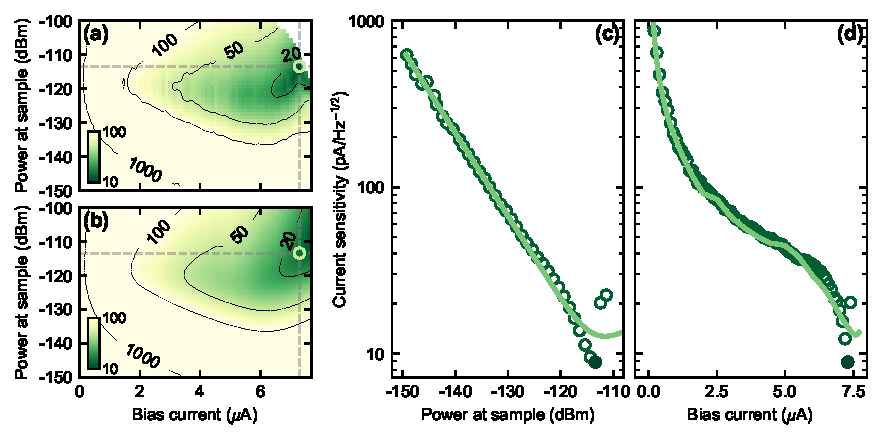
\includegraphics[width=\linewidth]{chapter-currentdetection/figures/Figure4}
	\caption{
		\textbf{Finding the best device sensitivity.}
		%
		Current sensitivity in \si{\pico\ampere\per\hertz\tothe{1/2}} versus bias current and input power, as measured (a) and calculated (b).
		%
		Dashed grey lines correspond to the linecuts in (c) and (d), circle marks the point of minimum measured sensitivity.
		%
		Color scale is logarithmic from 10 to 1000, black lines mark contour lines of sensitivity values as labeled.
		% 
		(b) Sensitivity at \SI{7.3}{\micro\ampere} versus pump power (vertical line in (a,b)).
		%
		We attribute discrepancies at high $P_\text{in}$ to differences in $\Delta$ between measurement and theory.
		%
		(c) Sensitivity at $P_\text{in}=\SI{-113}{dBm}$ versus bias current (horizontal line in (a,b)).
		%
		Circles: measured data, lines: model, full circle: minimum measured sensitivity.
		%
		\label{fig:figure4}
	}
\end{figure*}

\subsection{Limitations of present device and setup}\label{subsec:limitations}
% 
Optimum sensitivity would be achieved for zero pump detuning, maximum pump power and biasing the device close to $I_\text{c}$, cf. Fig.~\ref{fig:figure4}(a),(b).
% 
In our experiment we were unable to operate the device in a stable regime for bias currents greater than $0.9 \,I_\text{c}$, after which the JJ occasionally switched to the normal state, destroying the RF resonance.
% 
We attribute this to a significant ac current induced by the microwave drive on the order of \SI{1}{\micro\ampere}, cf. Supplemental Material Sec.~\ref{sec:accurrent}.
%
Together with the DC bias, the total current at the JJ reaches close to $I_\text{c}$, thus constraining the available parameter space.

Additionally, we observed exponential increase of the internal loss rate for large bias currents.
% 
These effects are presumably due to random phase diffusion across the junction and electrical interference in our setup, cf. Sec.~\ref{sec:lossrates} of the Supplemental Material~\cite{SeeSupplementalMaterial}.
% 
Most notably, at elevated bias currents spurious sidebands at integer multiples of \SI{50}{\hertz} appear in the measured spectra, which are due to insufficient isolation between the DC and RF electronics.
% 
Using the same approach as for the intended signal, we can quantify the current noise due to mains power to $\SI{170}{\pico\ampere}\approx I_\text{LF}/60$.
% 
Improving the setup should allow us to move to even higher bias currents, gaining in $\mathcal{S}_I$.
% 
In addition, the resonance frequency shift due to anharmonicity places an upper bound on the maximum input power.

In an optimized measurement, shifting the pump frequency with pump power in order to remain closer to resonance should allow us to gain more than \SI{10}{dB}, reaching a minimum of \SI{2.7}{\pico\ampere\per\hertz\tothe{1/2}}, cf. Sec.~\ref{sec:drive_shift} of the Supplemental Material~\cite{SeeSupplementalMaterial}.

\subsection{Modeled optimized device}

In order to improve $\mathcal{S}_I$, we propose a slightly changed circuit layout that follows naturally from the measured device and is immediately implementable:
% 
Instead of a transmission line shorted to ground by a single JJ, we propose to incorporate the Josephson inductance into the transmission line itself, by means of a diluted JJ metamaterial~\cite{planatUnderstandingSaturationPower2019}.
% 
The optimized design would then be a transmission line directly shorted to ground, with the CPW center conductor made up of a series of identical unit cells, each composed of a combination of linear and Josephson inductance ($L_0,L_\text{J}$) and a capacitance to ground ($C_0$), as depicted in Fig.~\ref{fig:figure5}(a).
% 
Following the approach to circuit quantization presented in Ref.~\cite{gelyQuCATQuantumCircuit2019} and methods from Refs.~\cite{noscheseTridiagonalToeplitzMatrices2013,niggBlackBoxSuperconductingCircuit2012,vool_introductionquantum_2017}, we derive the resonance frequency of this CPW as
% 
\begin{align}
\omega_0(I_\text{b})=\frac{\pi}{N\sqrt{C_0(L_\text{J}(I_\text{b})+L_0)}} \ ,
\end{align}
% 
in the limit of large $N$, as detailed in Sec.~\ref{sec:optimized} of the Supplemental Material~\cite{SeeSupplementalMaterial}.
% 
To maximize the responsivity $G_1$ of the device via maximizing the participation ratio $\eta_\text{J}=L_\text{J}/(L_0+L_\text{J})$ per unit cell, we propose a CPW with center conductor and gap sizes $1/10$ of the current design and a reasonably short unit cell length of \SI{1}{\micro\meter}.
% 
This would result in $L_0=\SI{842}{\femto\henry}$, $L_\text{J}=\SI{35.9}{\pico\henry}$ and $C_0=\SI{169}{\atto\farad}$ per unit cell, cf. Ref.~\cite{simonsCoplanarWaveguideCircuits2001} and Sec.~\ref{sec:optimized} of the Supplemental Material~\cite{SeeSupplementalMaterial}.
% 
For an initial resonance frequency at $\omega_0=2\pi\times\SI{7.5}{\giga\hertz}$, the device would require approximately 845 unit cells, resulting in a total device length of \SI{845}{\micro\meter}, much more compact than our present layout.
% 
Such an optimized device offers a significantly larger $G_1\approx\SI{4}{\giga\hertz\per\micro\ampere}$ with a relative frequency shift $\delta\omega_0/\omega_0\approx\SI{50}{\percent}$.
% 
Assuming the same internal losses as for our measured device and additionally increasing the external coupling, e.g. by reducing the shunt capacitor to $1/2$ of its current area, this device would be able to achieve sensitivities as low as \SI{0.17}{\pico\ampere\per\hertz\tothe{1/2}}, a factor of 54 improvement to our presented design, as shown in Fig.~\ref{fig:figure5}(b).

\begin{figure}[t]
	\centering
	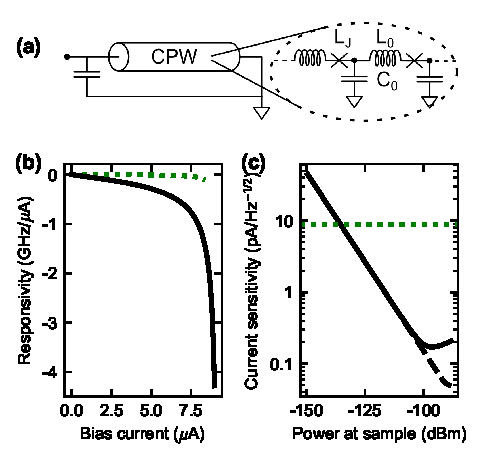
\includegraphics[width=.5\linewidth]{chapter-currentdetection/figures/Figure5}
	\caption{
		\textbf{Estimated sensitivities for optimized device design.}
		%
		(a) Instead of a linear CPW shorted to ground by a nonlinear Josephson junction, the optimized device is a diluted JJ meta material with a CPW center conductor based on a Josephson junction array, directly shorted to ground.
		%
		(b) Frequency responsivity $G_1$ for the optimized (solid line) and current device (dotted line).
		% 
		Due to the dominating Josephson inductance, the optimized device tunes further with bias current.
		% 
		(c) Predicted $\mathcal{S}_I$ for the optimized device.
		% 
		Dotted line indicates the minimum experimentally achieved sensitivity of \SI{8.9}{\pico\ampere\per\hertz\tothe{1/2}} with the present design.
		%
		For the JJ array CPW, we predict sensitivities as low as \SI{170}{\femto\ampere\per\hertz\tothe{1/2}} (solid line).
		%
		The sensitivity curves upwards for high pump powers due to the nonlinearity in the circuit.
		%
		Choosing the pump frequency to be continuously close to resonance for high drive powers, the predicted sensitivity would drop down to \SI{50}{\femto\ampere\per\hertz\tothe{1/2}} (dashed line).
		% 
		Parametric amplification could reduce the sensitivity one order of magnitude further by reducing the contribution of the noise of the cryogenic HEMT amplifier in the readout noise of the cavity.
		% 
		\label{fig:figure5}
	}
\end{figure}

We note that in an ideal experiment, the drive frequency should be tuned for increasing drive power in order to account for the Kerr-shift of the resonance to lower frequencies, thus minimizing $\Delta$ and maximizing $\alpha_0$.
% 
Implementing this measurement scheme would allow us to achieve sensitivities down to \SI{50}{\femto\ampere\per\hertz\tothe{1/2}}.
% 
Since this estimation does not take parametric amplification into account, we expect it to be an upper bound to the experimentally achievable $\mathcal{S}_I$:
% 
Utilizing quantum-limited parametric amplification built into the device would allow us to gain approximately \SI{20}{dB}~\cite{stehlikFastChargeSensing2015,pogorzalekHystereticFluxResponse2017,planatUnderstandingSaturationPower2019}, providing noise levels down to \SI{5}{\femto\ampere\per\hertz\tothe{1/2}}.

%%%%%%%%%%%%%%%%%%%%%%%%%%%%%%%%%%%%%%%%%%%%%%%%%%%%%%%%%%%%%%%%%%%%%%%%%%%%%%%%%%%%%%%%%%%%%%%%%%%%%%%%%%%%%%%%%%%%%%%%%
%%%%%%%%%%%%%%%%%%%%%%%%%%%%%%%%%%%%%%%%%%%%%%%%%%%%%%%%%%%%%%%%%%%%%%%%%%%%%%%%%%%%%%%%%%%%%%%%%%%%%%%%%%%%%%%%%%%%%%%%%
%%%%%%%%%%%%%%%%%%%%%%%%%%%%%%%%%%%%%%%%%%%%%%%%%%%%%%%%%%%%%%%%%%%%%%%%%%%%%%%%%%%%%%%%%%%%%%%%%%%%%%%%%%%%%%%%%%%%%%%%%
%%%%%%%%%%%%%%%%%%%%%%%%%%%%%%%%%%%%%%%%%%%%%%%%%%%%%%%%%%%%%%%%%%%%%%%%%%%%%%%%%%%%%%%%%%%%%%%%%%%%%%%%%%%%%%%%%%%%%%%%%
\section{Conclusion}

We presented a Josephson parametric upconverter and demonstrated current sensitivities down to \SI{8.9}{\pico\ampere\per\hertz\tothe{1/2}} which makes our compatible with TES readout, and derived an analytical model that accurately reproduces the measured data and is immediately applicable to other device architectures.
% 
We estimate that future devices using increased Josephson participation ratios, and using the intrinsic Kerr-nonlinearity for four-wave parametric amplification built into the detection cavity, should allow for an improved $\mathcal{S}_I\sim\SI{5}{\femto\ampere\per\hertz\tothe{1/2}}$, orders of magnitude better than state of the art KPUPs and limited by the fundamental quantum noise of the cavity.


%%%%%%%%%%%%%%%%%%%%%%%%%%%%%%%%%%%%%%%%%%%%%%%%%%%%%%%%%%%%%%%%%%%%%%%%%%%%%%%%%%%%%%%%%%%%%%%%%%%%%%%%%%%%%%%%%%%%%%%%%
%%%%%%%%%%%%%%%%%%%%%%%%%%%%%%%%%%%%%%%%%%%%%%%%%%%%%%%%%%%%%%%%%%%%%%%%%%%%%%%%%%%%%%%%%%%%%%%%%%%%%%%%%%%%%%%%%%%%%%%%%
%%%%%%%%%%%%%%%%%%%%%%%%%%%%%%%%%%%%%%%%%%%%%%%%%%%%%%%%%%%%%%%%%%%%%%%%%%%%%%%%%%%%%%%%%%%%%%%%%%%%%%%%%%%%%%%%%%%%%%%%%
%%%%%%%%%%%%%%%%%%%%%%%%%%%%%%%%%%%%%%%%%%%%%%%%%%%%%%%%%%%%%%%%%%%%%%%%%%%%%%%%%%%%%%%%%%%%%%%%%%%%%%%%%%%%%%%%%%%%%%%%%
\section*{Data availability}
All raw and processed data as well as supporting code for measurement libraries, data processing and figure generation is available in Zenodo~\cite{schmidtDataProcessingCurrent2020}.

\section*{Acknowledgements}
This project has received funding from the European Union Horizon 2020 research and innovation programme under grant agreement Nos. 681476 -- QOMD, 732894 -- HOT and 785219 -- GrapheneCore2.

%%%%%%%%%%%%%%%%%%%%%%%%%%%%%%%%%%%%%%%%%%%%%%%%%%%%%%%%%%%%%%%%%%%%%%%%%%%%%%%%%%%%%%%%%%%%%%%%%%%%%%%%%%%%%%%%%%%%%%%%%
%%%%%%%%%%%%%%%%%%%%%%%%%%%%%%%%%%%%%%%%%%%%%%%%%%%%%%%%%%%%%%%%%%%%%%%%%%%%%%%%%%%%%%%%%%%%%%%%%%%%%%%%%%%%%%%%%%%%%%%%%
%%%%%%%%%%%%%%%%%%%%%%%%%%%%%%%%%%%%%%%%%%%%%%%%%%%%%%%%%%%%%%%%%%%%%%%%%%%%%%%%%%%%%%%%%%%%%%%%%%%%%%%%%%%%%%%%%%%%%%%%%
%%%%%%%%%%%%%%%%%%%%%%%%%%%%%%%%%%%%%%%%%%%%%%%%%%%%%%%%%%%%%%%%%%%%%%%%%%%%%%%%%%%%%%%%%%%%%%%%%%%%%%%%%%%%%%%%%%%%%%%%%
%\appendix

\section{Input-output formalism}\label{app:inputoutput}

Starting from Eq.~\eqref{eq:Duffing-EOM}, with the steady-state solution $\alpha_0$, the reflection coefficient is given by
% 
\begin{align}
S_{11}=-1-\sqrt{\kappa_\text{e}}\frac{\alpha_0}{S_\text{in}}=-1+\frac{2\kappa_\text{e}}{\kappa+2i\Delta}
\end{align}
% 
where the second equality holds in the limit $\beta\rightarrow 0$ and which can be recognized as the usual reflection expression of circuit theory.

We now consider the case in which the cavity resonance frequency is a function of an additional current given by $I = I_\text{b} + \delta I$.
% 
With the resonance frequency given by Eq.~\eqref{eq:omega_Taylor}, the new equation of motion reads
% 
\begin{align}
\begin{split}
\dot{\alpha}=\left[ -i\left( \Delta -\sum_{m=1}^n G_m \delta I^m \right) - \frac{\kappa}{2} \right] \alpha \\
-i\beta\abs{\alpha}^2\alpha +\sqrt{\kappa_\text{e}}S_\text{in}\ .
\end{split}
\end{align}
% 
With the Ansatz for the intracavity field $\alpha(t)=\alpha_0+\delta\alpha(t)$ and assuming $\abs{\alpha}^2 \approx \alpha_0^2$ we get
% 
\begin{align}
\begin{split}
\delta\dot{\alpha}=\left[ -i\left( \Delta - \sum_{m=1}^n G_m \delta I^m \right) -\frac{\kappa}{2} \right] \delta\alpha \\
+i \alpha_0 \sum_{m=1}^n G_m \delta I^m \ .
\label{eq:delta-alpha-dot}
\end{split}
\end{align}
% 
Let the modulation in current be of the form
% 
\begin{align}
\delta I=I_\text{LF}\cos\Omega t = I_{-}e^{-i\Omega t} + I_{+}e^{+i\Omega t}
\label{eq:deltaIs}
\end{align}
% 
where $I_{-}=I_{+}=I_\text{LF}/2$.
% 
Our Ansatz for $\delta\alpha$ is consequently
% 
\begin{align}
\delta\alpha=\sum_{m=1}^n a_{-m}e^{-mi\Omega t} + a_{+m}e^{+mi\Omega t}\ .
\label{eq:deltaalpha}
\end{align}
% 
Inserting Eqs.~\eqref{eq:deltaIs},\eqref{eq:deltaalpha} into Eq.~\eqref{eq:delta-alpha-dot}, we can group the terms by their frequency components and equalize each component individually in order to solve for the sideband coefficients $a_{\pm m}$.
% 
Each sideband output field can then be calculated via
% 
\begin{align}
S_{\pm m} = \sqrt{\kappa_\text{e}} a_{\pm m}\ .
\end{align}
% 
We arrive at a compact result for the first order sidebands appearing at $\omega_0\pm1\Omega$:
% 
\begin{align}
S_{\pm 1} = \frac{\sqrt{\kappa_\text{e}}\alpha_0 G_1 I_\text{LF}}{-i\kappa+2(\Delta\pm\Omega)}\ .
\label{eq:input-output-first}
\end{align}

We calculated all $a_{\pm m}$ coefficients up to $m=3$ using \textit{Mathematica} v11.3.0.0 in the notebook \texttt{input-output formalism.nb}, which we subsequently converted to \textit{python3} code using the notebook \texttt{Export to Python.nb} located in Zenodo~\cite{schmidtDataProcessingCurrent2020}.

\section{Calculating the steady-state solution}\label{sec:Duffing}
% 
We can calculate $\alpha_0$ by solving Eq.~\eqref{eq:Duffing-EOM} for a large pump signal and treating the probe as a perturbation.
% 
Thus, let us assume that the solution has the form $\alpha(t)=\alpha_0 \exp [i\omega_\text{p} t]$ and the input signal $S_\text{in}(t) = S_\text{p}(t) =S_\text{p0} \exp [i(\omega_\text{p} t+\phi)]$ is the pump signal.
% 
Since we are only interested in the steady-state solution, let $S_\text{p0},\alpha_0 \in \mathbb{R}$.
% 
Inserting this into Eq.~\eqref{eq:Duffing-EOM}, we get
% 
\begin{align}
\left(i\Delta+\frac{\kappa}{2}\right)\alpha_0 + i\beta\alpha_0^3=\sqrt{\kappa_\text{e}}S_\text{p0}e^{i\phi}
\end{align}
% 
Multiplying this equation with its complex conjugate returns
% 
\begin{align}
\beta^2 \alpha_0^6 + 2\Delta\beta\alpha_0^4 + \left(\Delta^2+\frac{\kappa^2}{4}\right)\alpha_0^2 - \kappa_\text{e} S_\text{p0}^2 = 0\ .
\label{eq:polynom}
\end{align}
% 
While this third-order polynomial in $\alpha_0^2$ has multiple complex solutions, the ones relevant in our case are only real.
% 
In the high-power regime, our resonator will exhibit bifurcation and Duffing behavior, meaning there will be three real valued solutions to $\alpha_0^2$:
% 
The largest, median and smallest one corresponding to the high, middle and low amplitude branch, respectively.
% 
For a given input field $S_\text{p0}$ and detuning $\Delta$, the (up to three) solutions of this equation can be found either numerically or analytically.
% 
However, for the parameters used in our experiment, the solutions for $\alpha_0^2$ are identical because our drive remains outside of the bifurcation regime.
% 
We can then use the corrected intracavity field for obtaining the sideband amplitudes by replacing the value of $\alpha_0$ for the linear oscillator in Eq.~\eqref{eq:input-output-first}.

Furthermore, taking the resonance frequency as the point where $\partial\alpha_0/\partial\omega=0$, we can compute the frequency shift the cavity experiences as a result of the driving power by differentiating Eq.~\eqref{eq:polynom} with respect to $\omega$ as
% 
\begin{align}
\omega_0' = \omega_0 - \abs{\alpha_0}^2\beta\ .
\label{eq:Duffing-shift}
\end{align}


\section{Higher order terms}\label{app:higher-orders}
% 
Already for second order in $\delta I$, the prefactors are too complicated to write down in a short form, which is why we refer to the full analytical solutions in the \textit{Mathematica} notebook \texttt{input-output formalism.nb} located on Zenodo~\cite{schmidtDataProcessingCurrent2020}.
% 
We note that higher order corrections arising for terms in $\delta I^m$, have only negligible effects on the lower order forms.
% 
For the analysis in the main text, we therefore only make use of the closed form for the first order terms, and for the second order peaks in Fig.~\ref{fig:higher-order-peaks}(b-d), only the second order terms were used.

We observe higher order sidebands over a wide range of operating points, with an exemplary spectrum exhibiting both first and second order peaks plotted in Fig.~\ref{fig:higher-order-peaks}(a).
% 
Similar to Fig.~\ref{fig:figure3}(a), the second order sideband increases with DC bias current up to $I_\text{b}\approx 0.75\, I_\text{c}$ where the amplitude is limited by the increasing internal loss rate, cf. Fig.~\ref{fig:higher-order-peaks}(b).
%
As depicted in Fig.~\ref{fig:higher-order-peaks}(c), finite drive detuning strongly suppresses the sideband amplitude similar to the first order peaks.
% 
The power dependence, cf. Fig.~\ref{fig:higher-order-peaks}(c), also closely resembles the shape of the first order sideband, with maximum amplitude for high drive powers and subsequent decrease due to increasing drive detuning as a consequence of the downshift in resonance frequency due to the Kerr nonlinearity.

\begin{figure}[t]
	\centering
	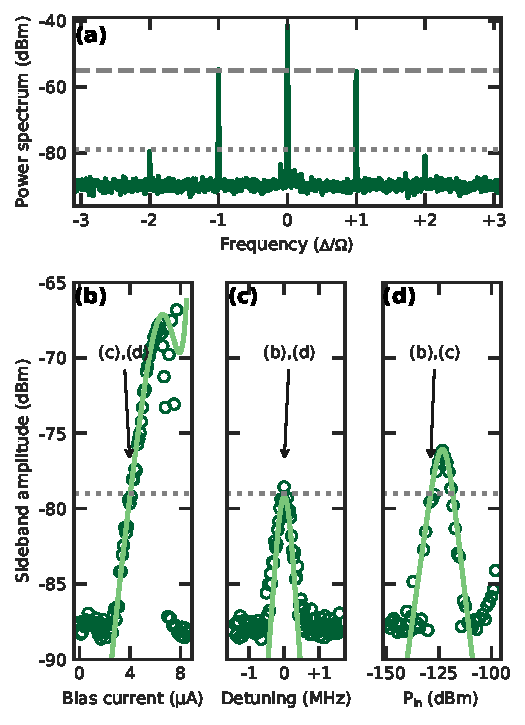
\includegraphics[width=.5\linewidth]{chapter-currentdetection/figures/SM_second_order_peak}
	\caption{
		\textbf{Exploring the parameter space for the second order sideband amplitude.}
		(a) Sideband height for changing bias current setpoint at fixed input power and zero detuning for varying bias current.
		(b) Sideband height for changing drive detuning at fixed input power and bias current.
		(c) Sideband height for changing input power at fixed bias current and detuning.
		Circles: measured data, solid lines: calculated amplitude via input-ouput theory, dotted grey line: calculated sideband amplitude at $I_0=\SI{4}{\micro\ampere}$, $\Delta=0$ and $P_\text{in}=\SI{-129}{dBm}$.
		Arrows indicate the setpoints for the other respective panels.
		(d) The power spectrum at the output at $I_0=\SI{4}{\micro\ampere}$, $\Delta=0$ and $P_\text{in}=\SI{-129}{dBm}$ containing the input pump signal at $\omega_0$ and the first and second order sidebands due to mixing at $\omega_0 \pm \Omega$ and $\omega_0 \pm 2\Omega$.
		Dotted grey line corresponds to the one in panels (a-c), dashed grey line corresponds to the one in Fig.~\ref{fig:figure3}.
	}
	\label{fig:higher-order-peaks}
\end{figure}

%%%%%%%%%%%%%%%%%%%%%%%%%%%%%%%%%%%
% Insert main.bbl contents here

%\input{main.bbl}


%%%%%%%%%%%%%%%%%%%%%%%%%%%%%%%%%%%
% Insert SM.tex contents here

\clearpage
\pagebreak
%\widetext

%\setcounter{equation}{0}
%\setcounter{figure}{0}
%\setcounter{table}{0}
%\setcounter{page}{1}
%\setcounter{section}{0}

%\renewcommand{\thepage}{S\arabic{page}}
%\renewcommand{\thesection}{S\Roman{section}}
%\renewcommand{\thetable}{S\Roman{table}}
%\renewcommand{\thefigure}{S\arabic{figure}}
%\renewcommand{\theequation}{S\arabic{equation}}
%\renewcommand{\bibnumfmt}[1]{[S#1]}
%\renewcommand{\citenumfont}[1]{S#1}

\section{Supplementary Material: Current detection using a Josephson parametric upconverter}

%\vspace{1em}

\section{Measurement setup}\label{sec:measurement}

\subsection{Wiring configuration}

All measurements were taken with the device mounted to the millikelvin stage of a \textit{Bluefors BF 400-D} dilution refrigerator with a base temperature of approximately \SI{15}{\milli\kelvin}.
% 
The measurement setup is sketched in Fig.~\ref{fig:setup}.
% 
We use in-house built, low-noise battery-powered electronics for DC measurements of the device: A voltage-controlled current source with an ideally infinite output impedance, and a voltmeter.
% 
For measurements involving current detection, we modulate the voltage controlled current source with an arbitrary waveform generator (AWG), model \textit{DG1022Z} from \textit{Rigol}.
% 
Microwave reflection measurements of the cavity are done using a vector network analyzer (VNA) from \textit{Agilent}, model \textit{PNA N5222A}.
% 
Signal generation and spectroscopy for current detection are done using signal generator \textit{SMB 100A} (SG) and analyzer \textit{FSV13} (SA), respectively, from \textit{Rohde \& Schwarz}.
% 
The VNA and SG paths are merged using directional couplers.
% 
Prior to the measurements on current detection, we calibrated the frequency dependent difference in attenuation between the signal paths VNA -- device under test (DUT) and SG -- DUT which we account for in all measurements and in the data analysis.

In order to minimize the influence of \SI{50}{\hertz} interference from mains powered equipment on our experiments, we place the DC electronics on an isolated rack and place all RF equipment on another one.
% 
We observed significant signal deterioration for elevated bias currents if the DC and RF electronics shared the same ground.
% 
For this reason, we placed additional DC blocks with separated inner and outer conductors on the RF input lines (PE8212 from \textit{Pasternack}).
% 
Note that for the LF current modulation, we need to galvanically connect the AWG to our current source, which in turn leads to a potential source of significant \SI{50}{\hertz} interference (see Sec.~\ref{sec:lossrates} for more elaborate discussion on this topic).

The DC lines are heavily filtered using $\pi$-filters inside the room-temperature electronics, and homemade copper powder and two-stage RC-filters on the baseplate of the dilution refridgerator.
% 
The \SI{-3}{dB} cut-off for these filters is at around \SI{30}{\kilo\hertz}, well above the chosen modulation frequency of \SI{1}{\kilo\hertz}.
%
To reduce the influence of stray magnetic fields, a passive $\mu$-metal shield surrounds the DUT and entire \SI{15}{\milli\kelvin} stage.

\begin{figure*}
	\centering
	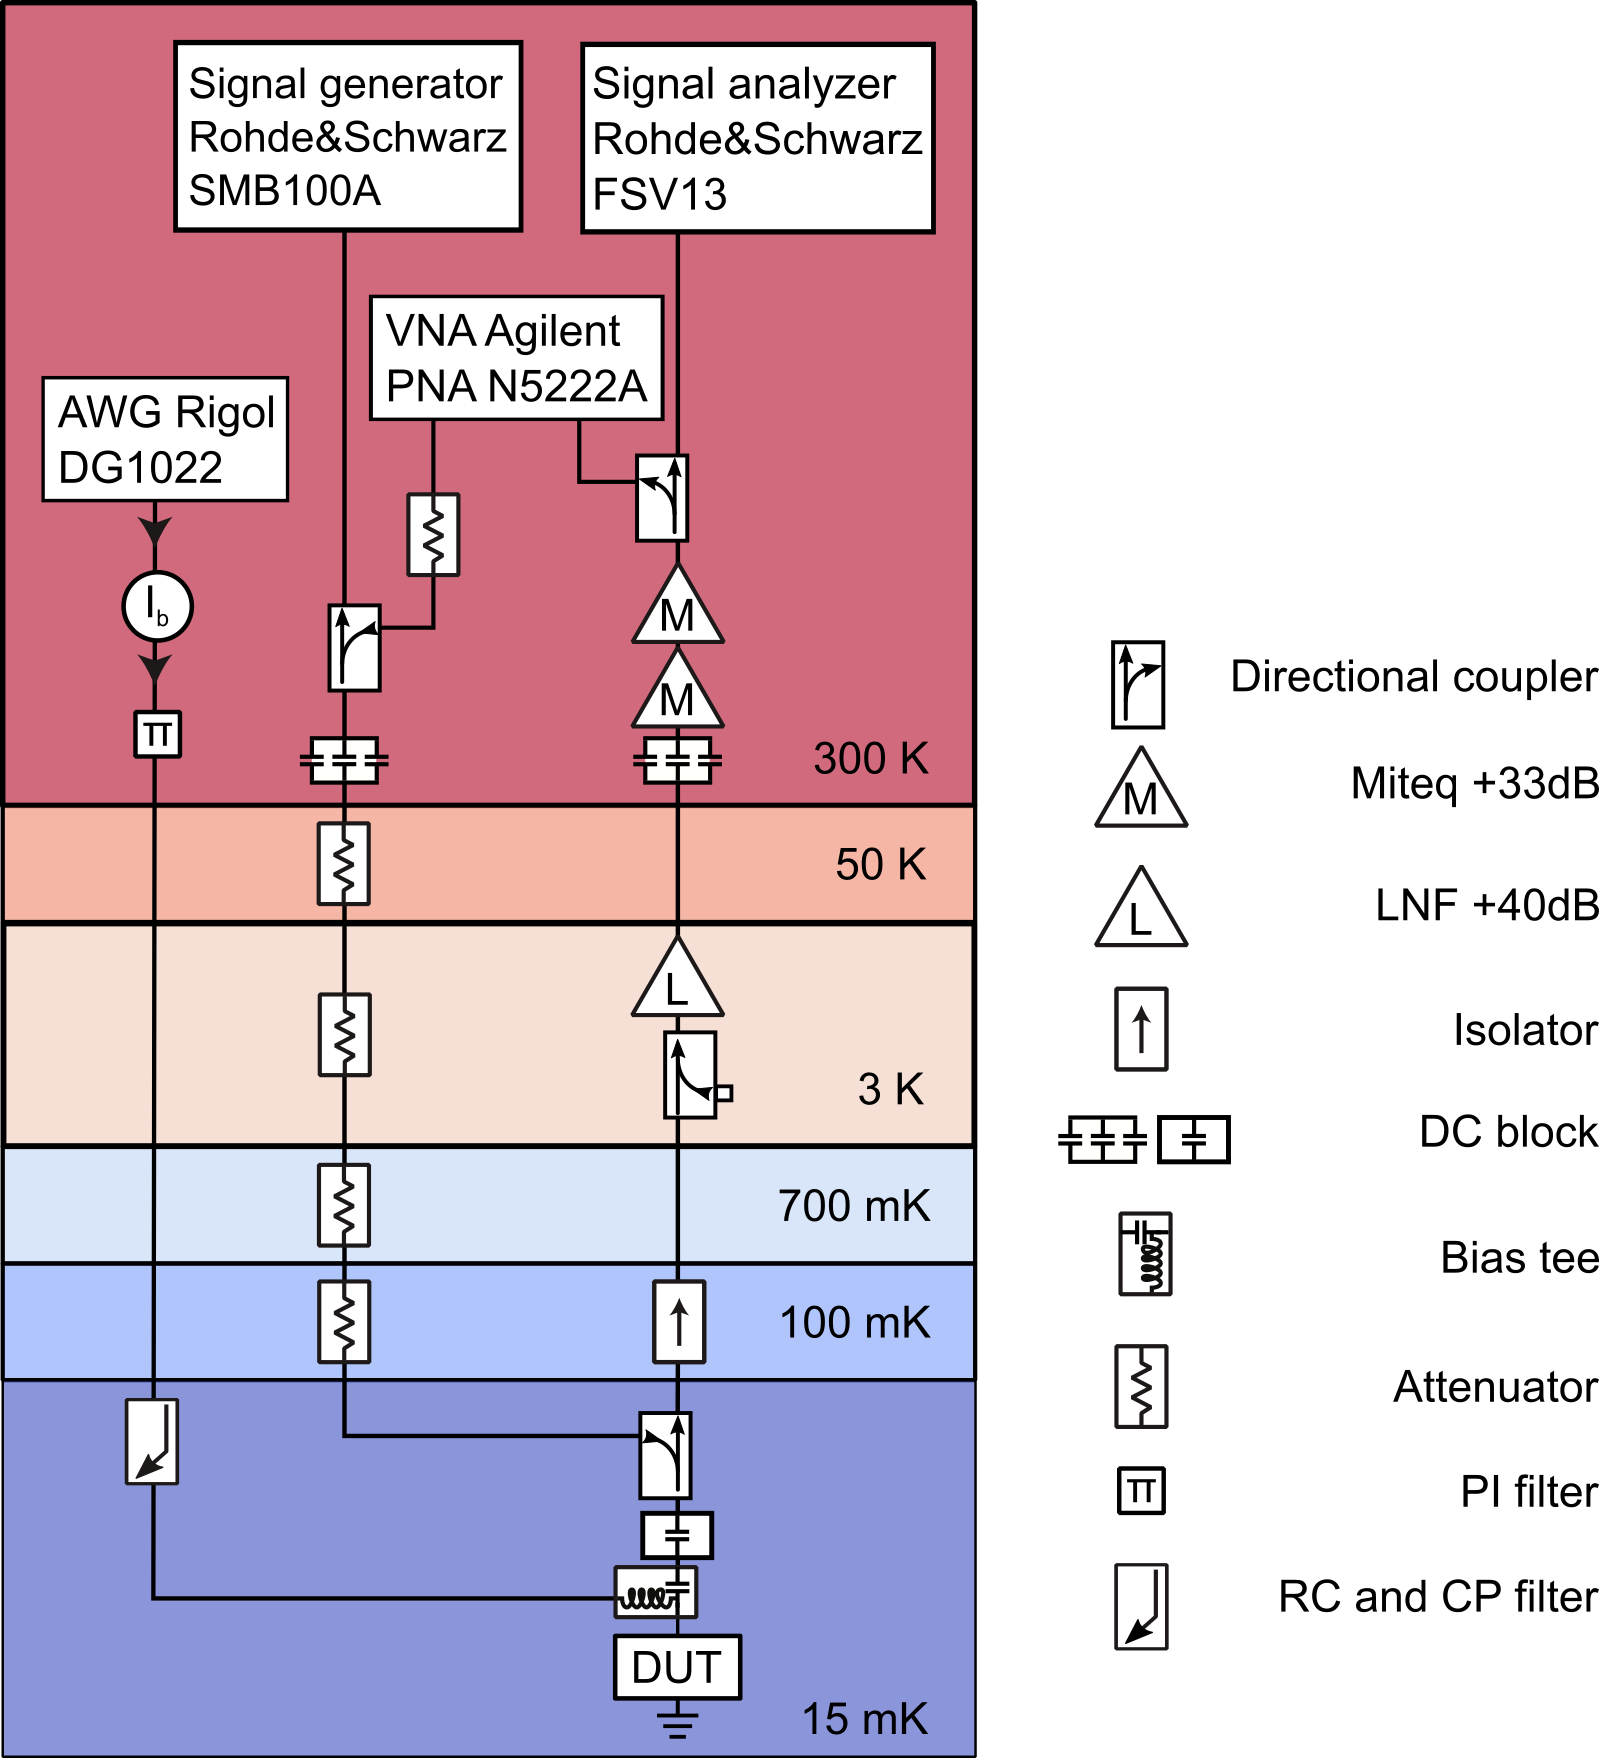
\includegraphics[width=\linewidth]{{chapter-currentdetection/figures/setup.svg}.png}
	\caption{
		\textbf{Measurement setup used for all measurements.}
		% 
		The directional coupler at the \SI{3}{\kelvin} stage was terminated by a \SI{50}{\ohm} load at the coupled port.
		% 
		The bias current source is battery powered and voltage controlled, while all other equipment is mains powered.
		% 
		DC blocks at room temperature isolate both center and outer conductor, while the ones at \SI{15}{\milli\kelvin} only isolate the center conductor.
		%
		From the millikelvin stage to the HEMT at \SI{3}{\kelvin}, we use superconducting cabling.
		%
		Not shown are a passive $\mu$-metal shield surrounding the millikelvin stage, as well as a cryogenic switch between DUT and bias-T to switch between the different samples on-chip, cf. Fig.~\ref{fig:fullchip}.
	}
	\label{fig:setup}
\end{figure*}

\subsection{Measurement protocol for current detection}
% 
The measurements on current detection were performed using the following measurement scheme:
% 
\begin{description}
	% 
	\item[1. Initialization and calibration] Turn off all outputs of RF instruments.
	%   
	Sweep the bias current back to zero and then to the next bias value.
	% 
	Set the VNA output power to low power and perform an $S_{11}$ measurement from \SI{7}{GHz} to \SI{8}{GHz}.
	% 
	From this measurement, determine the resonance frequency $f_0$ as the frequency at which $\abs{S_{11}}$ is minimum.
	\item[2. Current detection for fix pump power and detuning] Turn off the output of the VNA.
	% 
	Set the RF drive from the SG to low power and the drive frequency to $f_0$.
	% 
	Turn on the LF modulation ($I_\text{LF}=\SI{10}{\nano\ampere}$, $\Omega=2\pi\times\SI{1}{\kilo\hertz}$).
	% 
	Trigger the SA to perform one measurement.
	\item[3. Current detection for variable detuning] Keep the RF pump power at the same value and sweep the RF modulation frequency from $f_0-\SI{3}{\mega\hertz}$ to $f_0+\SI{3}{\mega\hertz}$ and for each detuning record the output signal using the SA.
	\item[4. Current detection for variable pump power] Set the RF frequency back to $f_0$.
	%   
	Sweep the RF pump power and for each pump power record the output signal using the SA.
	% 
	After each pump power measurement, reinitialize the bias current and find the resonance frequency again in order to reduce the number of "dead" cases in which the Josephson junction switched to the voltage state prematurely.
\end{description}

\subsection{Estimation of the attenuation and amplification chain}\label{sec:attenuation}

To estimate the attenuation chain, we use the thermal noise of our cryogenic high electron mobility transistor (HEMT) as a calibration source.
% 
The noise power due to the effective noise temperature $T_{\rm e}\approx2{\,\rm K}$ of the HEMT as given by the manufacturer is
% 
\begin{align}
P_{\rm N,in}'=k_{\rm B}T_{\rm e}\Delta f \approx \SI{2.761e-23}{\watt\per\hertz} \times \SI{1}{\kilo\hertz} \approx \SI{2.761e-20}{\watt} \approx \SI{-165.6}{dBm}\ ,
\label{eq:HEMTnoise}
\end{align}
% 
where $\Delta f=\SI{1}{\kilo\hertz}$ is the measurement bandwidth of our setup.
% 
By averaging over a few $S_{11}$ traces taken with the VNA in an area unaffected by our DUT, i.e. off-resonant to the cavity and thus leaving the background unaltered in power, we extract an average signal and standard deviation which we use to define the signal-to-noise ratio at the VNA, $\text{SNR}_\text{VNA}=\SI{34.5}{\decibel}$ for a VNA output power of \SI{0}{dBm}.

In our setup, the added noise from the HEMT dominates over other noise sources, which we deduce from an increase in noise level when powering up the HEMT with the room temperature amplifiers already on.
% 
Therefore, the SNR at the VNA is identical to the one at the HEMT output, and we deduce the power arriving at the HEMT input to be $P_{\rm in}=\SI{-131.3}{dBm}$. 
% 
Between DUT and HEMT, the signal travels a certain distance of cabling and passes through additional microwave components, cf. Fig.~\ref{fig:setup}.
% 
On the way, the signal will have been reduced by $X {\,\rm dB}$ due to the mentioned components, hence the power arriving at the HEMT will be $P_{\rm in}' = 10^{-X/10} P_{\rm in}$, which results in an estimated attenuation of \SI{129.3}{dB} of our VNA input line, assuming $X=\SI{2}{dB}$ of cable loss between sample and HEMT.

We deduce the total gain of our amplification chain by calculating the average noise power measured with the SA, $P_\text{N,SA}=\SI{-97.5}{dBm}$ in a \SI{1}{\hertz} bandwidth, and substracting from it the HEMT noise power $P_{\rm N,in}'=\SI{-195.6}{dBm}$ corresponding to the same bandwidth and the cable loss $X=\SI{2}{\decibel}$, resulting in a total gain of \SI{96.1}{\decibel} for the amplifier chain.

\section{Device fabrication}\label{sec:fabrication}

% 
The device is fabricated in a four-step process in the \textit{Kavli Nanolab} cleanroom of TU Delft, using a combination of electron beam lithography (EBL, EBPG5000+ from \textit{Raith}), liftoff, sputtering (AC450 from \textit{Alliance}), PECVD (PlasmaPro 80 from \textit{Oxford Instruments}) and dry-etching (Fluorine reactive ion etcher from \textit{Leybold Hereaus}).
% 
An optical micrograph of the fully packaged chip is shown in Fig.~\ref{fig:fullchip}.
% 
The geometric device parameters are given in Table~\ref{tab:geometry}.
% 
In the following we describe the fabrication step by step.
\begin{description}
	\item[Substrate] We use a double-side polished high-resistivity ($>\SI{6}{\kilo\ohm\centi\meter}$, light P/Boron doping, \SI{550}{\micro\meter} thickness) \SI{4}{inch} silicon wafer from \textit{IWS} as substrate for our device.
	% 
	The wafer is covered in positive electron beam resist (AR-P 6200.13, approximate thickness \SI{550}{\nano\meter}) and exposed to define the pattern for alignment and dicing markers.
	% 
	We sputter-deposit \SI{50}{\nano\meter} of Molybdenum-Rhenium (MoRe, RF magnetron sputtering in argon atmosphere from a \SI{60}{\percent} Mo-\SI{40}{\percent} Re target) and lift off the resist-protected areas using an anisole bath and strong ultrasonication, followed by multiple acetone and isopropanol baths.
	% 
	We subsequently cover the wafer with photoresist (HPR 504, \SI{1.2}{\micro\meter} thick) and dice it into \SI{14x14}{\milli\meter} chips for easier handling during fabrication.
	\item[Base layer] We pattern the Josephson junction together with the base layer and ground planes in a single lift-off step using AR-P 6200.09 (\SI{200}{\nano\meter}) and \SI{20}{\nano\meter} of sputtered Aluminum-Silicon (AlSi, reactive DC magnetron sputtering in argon atmosphere from a \SI{99}{\percent} Al-\SI{1}{\percent} Si target).
	% 
	Lift-off is done by placing the chip in the bottom of a beaker with room-temperature anisole and strong ultrasonication for a few minutes.
	\item[Dielectric layer] For the shunt dielectric layer, we deposit \SI{140}{\nano\meter} amorphous silicon at \SI{90}{\celsius} using PECVD.
	% 
	Patterning is done with EBL of a double-layer resist (PMMA 950K A4 and AR-N 7700.18) and reactive ion etching in a \ce{SF6 + He} atmosphere.
	% 
	The resist layers are in-situ removed using \ce{O2} plasma.
	\item[Top shunt plate] The top plate of the shunt capacitor is fabricated with an additional lift-off step using the same resist as for the alignment markers, and sputtering \SI{100}{\nano\meter} \ce{AlSi}.
	\item[Packaging] To fit our printed circuit board (PCB), the chip is again covered in photoresist and trimmed down to \SI{10x10}{\milli\meter}.
	% 
	After washing off the photoresist in a series of acetone and isopropanole baths, the chip is glued to our copper sample holder, to which the PCB is mounted, using cryogenic GE varnish.
	% 
	Electrical connections to the device are made using wedge-bonding on a Westbond wirebonder with aluminum wire bonds.
	% 
	We place a small copper lid on the chip to protect it from dirt and to suppress box modes of a bigger copper lid screwed onto the copper base, which accomodates the SMA connectors.
\end{description}

\begin{table}
	\caption{Geometric device parameters\label{tab:geometry}}
	\begin{tabular}{ccc}
		\hline \hline
		Symbol       & Description                                                                 & Value                            \\
		\hline
		$s$          & CPW center conductor                                                        & \SI{10}{\micro\meter}            \\
		%	\hline 
		$w$          & CPW gaps to ground                                                          & \SI{6}{\micro\meter}             \\
		%	\hline 
		$t$          & Base layer thickness                                                        & \SI{20}{\nano\meter}             \\
		%	\hline 
		$L_\text{g}'$ & Geometric inductance per length \cite{simonsCoplanarWaveguideCircuits2001}  & \SI{424}{\nano\henry\per\meter}  \\
		$C_0'$ & Geometric capacitance per length \cite{simonsCoplanarWaveguideCircuits2001} & \SI{169}{\pico\farad\per\meter}  \\
		$l$          & CPW length, from end of shunt to JJ                                         & \SI{6382}{\micro\meter}          \\
		%	\hline 
		$A_\text{s}$        & Shunt capacitor area                                                        & \SI{57800}{\micro\meter\squared} \\
		%	\hline 
		$t_\text{d}$        & Dielectric layer thickness                                                  & \SI{140}{\nano\meter}            \\
		\hline\hline
	\end{tabular}
\end{table}

\begin{figure}
	\centering
	\includegraphics[width=\linewidth]{{chapter-currentdetection/figures/fullchip-stitch.tif.resized}.png}
	\caption{
		\textbf{The full chip.}
		% 
		Microscope image of the full chip, wirebonded to the PCB used for measurements.
		% 
		The chip hosts four different devices:
		% 
		The CPW with single JJ discussed in the main text (bottom left), a reference cavity with the same geometry shorted to ground (top left), and two devices shorted to ground by superconducting interference devices (SQUIDs) with loop sizes \SI{8x9}{\micro\meter} (top right) and \SI{5x5}{\micro\meter} (bottom right).
		% 
		Structures in the chip center are used for room-temperature DC tests.
		% 
		Chip size is \SI{10x10}{\milli\meter}.
	}
	\label{fig:fullchip}
\end{figure}

\section{General device parameters}\label{sec:general}

\subsection{Reflection coefficient}\label{sec:general-S11}
% 
The reflection coefficient of a transmission line with a shunt capacitor to ground on the input side and shorted to ground on the far end is given by
% 
\begin{align}
S_{11}(\omega,\kappa_\text{i},\kappa_\text{e}) = \frac{\kappa_\text{e}-\kappa_\text{i}-2i\Delta}{\kappa_\text{e}+\kappa_\text{i}+2i\Delta} = -1+\frac{2\kappa_\text{e}}{\kappa+2i\Delta}
\label{eq:S11simple}
\end{align}
% 
with the detuning from resonance, $\Delta=\omega-\omega_0$ and the internal, external and total loss rates $\kappa_\text{i}$, $\kappa_\text{e}$ and $\kappa=\kappa_\text{e}+\kappa_\text{i}$.
%
Broadly speaking, the external loss rate describes signal loss of the DUT to the feedline, while the internal loss rate describes losses due to effects like radiation or dielectrics.
%
Following Ref.~\cite{bosmanBroadbandArchitectureGalvanically2015c}, we infer $\kappa_\text{e} = 2/(\pi\omega_0 Z_0^2 C_\text{s}^2)$ for a CPW with impedance $Z_0$ matched to that of a feedline.
%
There is no analytical expression for $\kappa_\text{i}$.

% 
The real response function is however distorted by the complex microwave background which arises due to impedance mismatches in our measurement setup, as can be seen in Fig.~\ref{fig:s11fitabs}(a).
% 
For this reason, we model the measured $S_{11}$ spectra using the above model for an ideal device multiplied by a complex microwave background and a rotation in the complex plane:
% 
\begin{align}
S_{11}'(\omega,\kappa_\text{i},\kappa_\text{e},\theta) & = \left( a+b\omega+c\omega^2 \right) e^{i(a' + b' \omega)}  \left\{e^{i\theta}\left[S_{11}(\omega,\kappa_\text{i},\kappa_\text{e})+1\right]-1\right\}
\label{eq:S11full}
\end{align}
% 
Our fitting algorithm first detects the resonance as frequency corresponding to the maximum phase derivative and fits the background signal by removing a certain window around the resonance frequency.
% 
In a second step, it fits the modified model to the full data set keeping the background parameters fixed, and finally refits all background and model parameters once more starting from the previously fitted values.
% 
A result of this fitting procedure, with background removed, is shown in Fig.~\ref{fig:s11fitabs}(b,c).

\begin{figure}
	\centering
	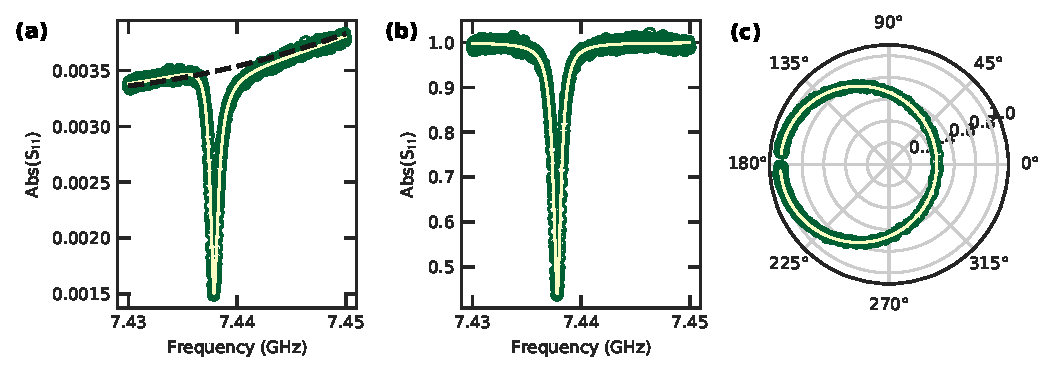
\includegraphics[width=\linewidth]{chapter-currentdetection/figures/SM_reflection_coefficient}
	\caption{
		\textbf{Data and fit of the reflection coefficient.}
		%
		(a) Absolute value of $S_{11}$ as measured (markers) with fit (solid line) taking into account background (dashed line).
		%
		(b) Absolute value of the reflection coefficient $S_{11}$ versus frequency after removing the oscillating background.
		%		
		(c) Polar plot of the absolute value of $S_{11}$ versus phase, without background and rotation in the complex plane.
		% 
		Markers: data, solid lines: fits according to Eq.~\eqref{eq:S11simple}.
		\label{fig:s11fitabs}
	}
\end{figure}


\subsection{Kinetic inductance estimation}\label{sec:Lk}

% 
Our AlSi films have a significant kinetic inductance contribution due to their small thickness of only \SI{20}{nm}.
% 
We estimate the kinetic inductance fraction by performing a finite element electromagnetic simulation using \textit{Sonnet} v16.56 (Sonnet Software Inc., 2018) of the reference device (shorted to ground on the same chip, thus excluding the Josephson inductance) which results in an expected resonance due to only geometry at $\omega_\text{g}=2\pi\times\SI{8.83}{\giga\hertz}$.
% 
We compare this value with the measured value of $\omega_\text{k}=2\pi\times\SI{7.56}{\giga\hertz}$.
% 
The kinetic inductance fraction is given by~\cite{gaoExperimentalStudyKinetic2006}
% 
\begin{align}
\eta_\text{k} = \frac{L_\text{k}'}{L_\text{k}'+L_\text{g}'}=1-\left(\frac{\omega_\text{k}}{\omega_\text{g}}\right)^2
\end{align}
% 
which has a value of $0.267$ in our device, hence $L_\text{k}'=\SI{154}{\nano\henry\per\meter}$.
%
This changes the characteristic impedance of our CPW from the geometric value of \SI{50.1}{\ohm} to \SI{58.5}{\ohm}.
% 
Kinetic inductance also increases as a function of DC bias current via $L_\text{k}(I)=L_\text{k}(0)\left[1+(I/I_*)^2\right]$ with the characteristic current $I_*$ \cite{annunziataTunableSuperconductingNanoinductors2010b}.
% 
The resulting downshift of the resonance frequency can be described by
% 
\begin{align}
\omega_0(I_\text{b}) = \frac{\omega_0(0)}{\sqrt{1+\eta_\text{k}I_\text{b}^2/I_*^{2}}} \ .
\label{eq:kinetic-tuning}
\end{align}
% 
We emphasize however that in the JJ device, the sheet kinetic inductance is not the relevant tuning parameter:
% 
Biasing the reference device up to \SI{10}{\micro\ampere} does not show a trend; instead the fluctuations in $f_0$ remain within the fitting errors, cf. Fig.~\ref{fig:reference-current}(a).
% 
Only when applying bias currents up to \SI{200}{\micro\ampere}, well beyond the values used for the measurements presented in the main text, does the resonance frequency of the reference device shift to lower frequencies, as shown in Fig.~\ref{fig:reference-current}(b).
% 
We fit the data using Eq.~\eqref{eq:kinetic-tuning}, extracting $I_*\approx\SI{7.35}{\milli\ampere}$.
% 
This supports our claim that we can exclude kinetic inductance as an additional source of tuning the resonance frequency via applied bias currents and instead identify the Josephson inductance as the relevant tuning parameter.


\begin{figure}
	\centering
	\includegraphics[width=\linewidth]{chapter-currentdetection/figures/SM_frequency_shift_ref}
	\caption{
		\textbf{Frequency shift of the reference CPW shorted to ground.}
		% 
		(a) Within the bias range for the device in the main text, $I_\text{0,max}=\SI{8}{\micro\ampere}$, the fluctuations in resonance frequency of the reference device are not due to kinetic inductance but remain within the range of our fit errors for the resonance frequency.
		% 
		(b) Biasing the reference resonator up to \SI{200}{\micro\ampere} allows us to extract the characteristic current for the kinetic inductance of the superconductor, $I_*\approx\SI{7.35}{\milli\ampere}$.
		% 
		Markers: data with error bars, solid line: fit to Eq.~\eqref{eq:kinetic-tuning}, dashed lines: range of applied bias currents for JPUP experiments in main text.
	}
	\label{fig:reference-current}
\end{figure}

% \subsection{Josephson inductance versus current}\label{sec:LJ}

% Assuming the Josephson junction can be described by a sinusoidal current phase relation (CPR), we can obtain an analytical expression for the phase drop across the Josephson junction $\delta$ for a given critical current $I_\text{c}$ and bias current $I_\text{b}=I_\text{c}\sin\delta$, which we can insert into the expression for the Josephson inductance,
% \begin{align}
% 	L_\text{J}(\delta)=\frac{\Phi_0}{2\pi} \left( \frac{\partial I_\text{b}}{\partial \delta} \right)^{-1} = \frac{\Phi_0}{2\pi I_\text{c} \cos\delta} \\
% 	\Rightarrow L_\text{J}(I_\text{b}) = \frac{\Phi_0}{2\pi \sqrt{I_\text{c}^2-I_\text{b}^2}}
% 	\label{eq:Lj-of-I}
% \end{align}
% with the flux quantum $\Phi_0=\frac{h}{2e}$ where $h$ is Planck's constant and $e$ the elementary charge.

\subsection{Resonance frequency versus current due to Josephson inductance}\label{sec:resfit}

% 
Adapting the calculation for a Josephson terminated transmission line cavity given in Ref.~\cite{pogorzalekHystereticFluxResponse2017} to our device, we find for the current dependence of the cavity resonance frequency
% 
\begin{align}
\omega_0(I_\text{b})=\omega_{\lambda/2}\,\frac{L_\text{r}+L_\text{J}(I_\text{b},I_\text{c})}{L_\text{r} + 2L_\text{J}(I_\text{b},I_\text{c})}\ ,
\end{align}
% 
with $L_\text{r}$ the total device inductance, $\omega_{\lambda/2}$ the resonance frequency without the JJ and $L_\text{J}$ the Josephson inductance given in Eq.~\eqref{eq:Lj-of-I} of the main text.
% 
We use this model to fit the measured resonance frequencies and extract $\omega_{\lambda/2}=2\pi\times\SI{7.515}{\giga\hertz}$, $L_\text{r}=\SI{3.401}{\nano\henry}$ and $I_\text{c}=\SI{9.157}{\micro\ampere}$.
% 
From the device geometry and kinetic inductance estimation, we expect $L_\text{r}=(L_\text{g}'+L_\text{k}')l=\SI{3.689}{\nano\henry}$, which is in acceptable agreement with the fit value.

\section{On the hysteresis of switching currents in our DC measurements}\label{sec:hysteresis}
% 
Accodring to a simple RCSJ model, hysteresis in Josephson junctions should occur only for JJ quality factors $Q=R\sqrt{2eI_\text{c} C_\text{J}/\hbar} > 1$, with the junction capacitance $C_\text{J}$~\cite{tinkhamIntroductionSuperconductivity1996}.
% 
We perform finite element simulations with \textit{Sonnet} v16.56 (Sonnet Software Inc., 2018) to estimate the stray capacitance of the metal leads in direct vicinity of the JJ (two \SI{1x1}{\micro\meter} pads separated by \SI{200}{\nano\meter}) to be $C_\text{J}=\SI{5.2}{\femto\farad}$.
% 
Together with $R=\SI{108}{\ohm}$ and $I_\text{c}=\SI{9.157}{\micro\ampere}$, the junction would have $Q\approx1.3$.
% 
For $Q \gtrsim 1$, the ratio between retrapping and critical current can be approximated as $I_\text{r}/I_\text{c}=4/\pi Q$.
% 
Hence, in order to satisfy our measured values, $Q=4/\pi\times I_\text{c}/ I_\text{r}\approx1.91$, which would be reached for $C_\text{J}\approx\SI{11}{\femto\farad}$.
% 
Likely, the geometric capacitance of the CPW and the surrounding ground planes significantly contributes and dominates the circuit capacitance:
% 
Already including a \SI{50}{\micro\meter} portion of the CPW increases $C_\text{J}$ to \SI{14}{\femto\farad}, satisfying this requirement.
% 
Additionally, we note that local heating in the junction area can also play a significant role, reducing $I_\text{r}$ further~\cite{skocpolSelfHeatingHotspots1974,hazraHysteresisSuperconductingShort2010,kumarReversibilitySuperconductingNb2015}.

\section{On the increased loss rates for increased bias current}\label{sec:lossrates}

% 
We observed an increase in the internal and external loss rates of the JJ terminated device for increased bias current, as can be seen in Fig.~\ref{fig:lossratesvscurrent}(a).
% 
We can fit the loss rates quite accurately with a phenomenological exponential model of the form
% 
\begin{align}
\kappa(I_\text{b}) = \kappa_0 + \kappa_1 \exp\left[\frac{I_\text{b}}{I_{\sim}}\right]\ .
\label{eq:lossrates}
\end{align}
% 
The extracted parameters for the device presented in the main text are given in Tab.~\ref{tab:lossrates}.
% 
While $\kappa_\text{e}$ should not directly depend on bias current, we do observe a slight increase, possibly due to changes in the impedance, linewidth broadening due to the increased $\partial\omega_0/\partial I_\text{b}$ or shifting the cavity through cable resonances.
% 
Regarding the increase in internal loss rate, we identified the following mechanisms as most likely:
% 
\begin{description}
	\item[Electrical interference] While we physically disconnect all mains-powered equipment from our battery powered DC electronics, and placed DC blocks for both inner and outer conductors on the RF inputs to the fridge, we still notice a significant amount of \SI{50}{\hertz} interference on the measured spectra for high bias currents, cf. Fig.~\ref{fig:50hzinterference}(a).
	%   
	We calculate the magnitude of the spurious signals to be approximately \SI{170}{\pico\ampere}, which corresponds to \SI{1.7}{\percent} of $I_\text{LF}$ or $1.86\times 10^{-5}\, I_\text{c}$.
	% 
	We assume that this interference is always present but only has noticeable effects for large $\partial\omega_0/\partial I_\text{b}$.
	% 
	Since our RF spectroscopy measurement takes more than \SI{1}{\second}, the measured linewidth is effectively broadened by the moving cavity, induced by small-scale \SI{50}{\hertz} modulations.
	%
	While more insight could potentially have been gained by performing switching histogram measurements, the small magnitude of the spurious interference compared to the JJ switching current should only slightly affect DC measurements.
	
	Note that the situation is significantly worse for an unoptimized setup, when noise couples to the DC electronics via a shared ground.
	%
	This is the case when bolting the power strip (into which the VNA and SA are plugged in) to the metal housing of the rack on which the battery-powered DC electronics sit.
	% 
	In this case, the cavity spectrum is extremely broadened and starts to resemble two dips for high $I_0$, severely limiting the tuning range (c.f. Fig.~\ref{fig:50hzinterference}(b) without, and Fig.~\ref{fig:figure1}(f) of the main text with isolation of the battery electronics from mains powered equipment).
	% 
	We estimate the interfering current signal for this case to be \SIrange{150}{250}{\nano\ampere}, significantly limiting any device operation in either DC or RF.
	% 
	The measurement setup could be further improved by choosing a LF modulation frequency which is not a higher order multiple of \SI{50}{\hertz}, such as \SI{1111}{\hertz}, instead of \SI{1000}{\hertz}.
	
	We note that there might be other frequencies at which interfering signals couple into our device.
	%		
	For example, the acoustic vibrations of the pulse tube needed to provide continuous cooling power in a dry dilution refrigerator have been shown to induce periodic current spikes in the \SIrange{5}{10}{\kilo\hertz} range of up to a few \si{\nano\ampere}~\cite{kalraVibrationinducedElectricalNoise2016b}, which would lead to a significant increase in $\kappa_\text{i}$.
	%
	Since our DC lines use only a small portion of coaxial cable at the mK stage and are otherwise twisted loom pairs up to room temperature, we expect this contribution to be small.
	% 
	Nevertheless, current noise by itself cannot completely account for the observed increased loss rates with bias current because $\kappa_\text{i}(I_\text{b})$ is not simply proportional to $\partial\omega_0/\partial I_\text{b}(I_\text{b})$.
	\item[Phase diffusion] The shorted reference device exhibits constant $\kappa_\text{i}$ and $\kappa_\text{e}$ upon DC bias up to \SI{200}{\micro\ampere}, at which point the mixing chamber starts to heat as we surpass the cooling power  of \SI{14}{\micro\watt} for the \textit{LD400 Bluefors} since the power dissipated in our \SI{2.7}{\kilo\ohm} low-pass filters reaches up to \SI{108}{\micro\watt}.
	% 
	In contrast, the temperature did not increase when measuring the JJ device.
	% 
	We therefore rule out quasiparticles (due to radiation or thermal excitations \cite{tinkhamIntroductionSuperconductivity1996}) in the CPW as a significantly contributing loss mechanism.
	% 
	Instead, phase diffusion across the JJ can play a significant role as the bias current approaches $I_\text{c}$.
	% 
	Applying a DC bias current tilts the Josephson energy potential, enhancing the chance of phase-slip and quantum tunneling events, which can lead to dissipation even without switching to the normal state, as long as the phase particle is able to settle in the next washboard-potential minimum \cite{kiviojaWeakCouplingJosephson2005}.
	%	\item [Fano interference] Due to impedance mismatches between the directional coupler and our sample, there can be interference between incoming and outgoing waves.
	%	These show up in the microwave spectroscopy as Fano lineshapes, which makes extracting the internal and external device linewidths notoriously difficult.
\end{description}

\begin{table}
	\caption{Extracted loss rate parameters for the main text device.\label{tab:lossrates}}
	\begin{tabular}{cccc}
		\hline \hline
		Loss rate         & $\kappa_0/2\pi$ (\si{\kilo\hertz}) & $\kappa_1/2\pi$ (\si{\hertz}) & $I_{\sim}$ (\si{\nano\ampere}) \\
		\hline
		Internal & $256.16 \pm 3.74$             & $78.41 \pm 11.86$      & $777.89 \pm 11.96$             \\
		%	\hline 
		External & $537.41 \pm 2.11$             & $0.021 \pm 0.035$      & $487.43 \pm 52.40	$             \\
		\hline \hline
	\end{tabular}
\end{table}

\begin{figure}
	\centering
	\includegraphics[width=\linewidth]{chapter-currentdetection/figures/SM_lossrates}
	\caption{
		\textbf{Bias current dependent cavity loss rates.}
		% 
		(a) Internal ($\bigcirc$) and external ($\square$) loss rates versus bias current of the JJ terminated device. The measured values can be described by the exponential model (lines) from Eq.~\eqref{eq:lossrates}.
		% 
		(b) Internal ($\bigcirc$) and external ($\square$) loss rates of the reference device.
		% 
		We do not observe an increase in loss rate up to \SI{200}{\micro\ampere}.
		% 
		(c) Base temperature during measurement of (b).
		% 
		As we exceed the fridge cooling power, the mixing chamber plate heats up, but without any clear effect on $\kappa_\text{i}$ and $\kappa_\text{e}$.
	}
	\label{fig:lossratesvscurrent}
\end{figure}

\begin{figure*}
	\centering
	\includegraphics[width=\linewidth]{chapter-currentdetection/figures/SM_50Hz_interference}
	\caption{
		\textbf{Mains power interference.}
		% 
		(a) Current-mixing output spectrum taken at \SI{7.1}{\micro\ampere} bias current for the device in the main text.
		% 
		Peaks at zero frequency and $\pm\SI{1}{\kilo\hertz}$ correspond to the cavity-resonant continuous wave pump tone and the mixing sidebands, respectively.
		% 
		Even with mains powered equipment separated from battery electronics, spurious peaks appear at integer multiples of \SI{50}{\hertz}, corresponding to current signals of approximately \SI{170}{\pico\ampere}.
		% 
		(b) $\abs{S_{11}}$ measurements of the same device in the same cooldown, but with \SI{50}{\hertz} interference coupling to the DC electronics via a common ground.
		% 
		(c) Linecuts through (b) at various bias currents as indicated in (b).
		% 
		For high bias currents, the resonance splits into two dips, clearly hinting at significant current noise, which we estimate to be \SIrange{150}{250}{\nano\ampere}.
	}
	\label{fig:50hzinterference}
\end{figure*}

\section{Estimating the AC current at the junction}\label{sec:accurrent}

The current along a $\lambda/2$ resonator shorted to ground on both ends is given by
%
\begin{equation}
I(x) = I_0\cos{\left(\pi\frac{x}{l_0}\right)}
\end{equation}
%
where $l_0$ is the physical length of the cavity on the chip, $I_0$ is the current amplitude in the current antinodes and $x$ is the coordinate along the resonator with $0 \leq x \leq l_0$.
%
To find the peak current for a given intracavity energy $\alpha_0^2$, we equalize the total energy related to the current with the intracavity energy
%
\begin{equation}
\alpha_0^2 = \frac{1}{2}\int_0^{l_0}L' I^2(x)\text{d}x = \frac{l_0}{4}L' I_0^2
\end{equation}
%
The peak microwave current in the antinode is therefore given by
%
\begin{equation}
I_0 = \sqrt{\frac{4 \alpha_0^2}{L' l_0}}.
\end{equation}
%
The intracavity energy for a resonant drive on the other hand is given by
%
\begin{equation}
\alpha_0^2 = 4P_\text{in} \frac{\kappa_\text{e}}{\kappa^2}
\end{equation}
%
in the linear regime.
%
For an input power of \SI{-110}{dBm}, we then get a microwave current of $I_0\approx\SI{1.86}{\micro\ampere}$ using $\kappa_\text{e} = 2\pi\times\SI{0.5}{\mega\hertz}$ and $\kappa = 2\pi\times\SI{1}{\mega\hertz}$ as observed for about $I_\text{b} \approx \SI{7}{\micro\ampere}$.
%
From the impedance of the junction at this operation point $Z_\text{J} \approx \SI{3i}{\ohm}$, we estimate that the actual current through the junction is reduced to about 0.8 to 0.9 of the antinode current due to the boundary condition being not an ideal short.
%
The intracavity microwave current is therefore capable of explaining the suppression of the DC critical current (premature switching) with increasing microwave power.


\section{Difference between first order red and blue sidebands}\label{sec:bluered}
% 
As derived in the main text, to first order in $\delta I$, the coefficients describing the sideband amplitudes are
% 
\begin{align}
a_{\pm 1} & = \frac{\alpha_0 G_1 I_\text{LF}}{-i\kappa+2(\Delta\pm\Omega)} \ .
\label{eq:input-output-first}
\end{align}
% 
Without changing the device, our peak height will increase if we modulate the current stronger ($I_\text{LF}\uparrow$) or slower ($\Omega\downarrow$), and by pumping harder ($S_\text{in}\uparrow$).
% 
With the same setup, increasing the current responsivity ($G_1\uparrow$) would likewise enhance the peak height.
% 
Moreover, for small LF modulations $\Omega\ll\kappa$, the peaks for red and blue sidebands should be equal in amplitude.
% 
In fact, the absolute difference between the two sidebands scales with
% 
\begin{align}
\abs{a_{-1}}^2-\abs{a_{+1}}^2 &\propto \frac{16 \Delta \Omega}{\left( \kappa^2+4(\Delta+\Omega)^2 \right)\left( \kappa^2+4(\Delta-\Omega)^2 \right)} \rightarrow 0 \ ,
\end{align}
for $\kappa \gg \Omega$.
% 
Our experiments with $\kappa \gtrsim 2\pi\times\SI{750}{\kilo\hertz} \gg \Omega = 2\pi\times\SI{1}{\kilo\hertz}$ support this statement, as we did not observe systematic differences between red and blue sidebands (cf Fig.~\ref{fig:plusminus}) over the entire parameter space.

\begin{figure}
	\centering
	\includegraphics[width=\linewidth]{chapter-currentdetection/figures/SM_plusminus}
	\caption{
		\textbf{Comparison of blue and red sideband.}
		% 
		Current sensitivity in \si{\pico\ampere\per\hertz\tothe{1/2}} versus bias current and input power, as measured for $-\Omega$ (a, cf. Fig.~\ref{fig:figure4} of the main text) and $+\Omega$ (b).
		% 
		Dashed grey lines correspond to the linecuts in (c) and (d), circle marks the point of minimum measured sensitivity.
		% 
		(b) Sensitivity at \SI{7.3}{\micro\ampere} versus pump power (vertical line in (a,b)).
		% 
		(c) Sensitivity at \SI{-113}{dBm} versus bias current (horizontal line in (a,b)).
		% 
		$\circ$: $-\Omega$ sideband, $\star$: $+\Omega$ sideband.
		% 
		Minimum sensitivities are \SI{8.90}{\pico\ampere\per\hertz\tothe{1/2}} and \SI{9.52}{\pico\ampere\per\hertz\tothe{1/2}}, respectively.
		% 
		Within the traced out parameter space, we observed no systematic differences between red and blue first order sidebands.
	}
	\label{fig:plusminus}
\end{figure}


\section{Current detection in the high power regime}\label{sec:high_powers}

\subsection{Driving the cavity on resonance for high powers}\label{sec:drive_shift}
To counteract acquired detuning from the downshift in resonance frequency for high pump powers due to the device nonlinearity, in an ideal measurement configuration the drive tone would also be shifted correspondingly.
% 
As depicted in Fig.~\ref{fig:Duffing-on-res}, in such a situation, the sideband amplitude would keep increasing by more than \SI{10}{\decibel}, resulting in a minimum $\mathcal{S}_I=\SI{2.6}{\pico\ampere\per\hertz\tothe{1/2}}$.

\begin{figure}
	\centering
	\includegraphics[width=\linewidth]{chapter-currentdetection/figures/SM_Duffing_on_resonance}
	\caption{
		\textbf{Driving the cavity on resonance.}
		% 
		(a) Data (circles) and model with (solid line) and without (dashed line) detuning of the first order sideband amplitude at $I_0=\SI{4}{\micro\ampere}$, cf. Fig.~\ref{fig:figure3}(c) of the main text.
		% 
		Tuning the drive to be matched to the resonance results in a further increased sideband amplitude of more than \SI{10}{\decibel}.
		% 
		(b) Data (circles) and model (solid line) of the first order sideband amplitude at $P_\text{in}=\SI{-113}{dBm}$, cf. Fig.~\ref{fig:figure4}(d) of the main text.
		% 
		Dashed line corresponds to modelled sensitivity at maximum drive power with shifted drive frequency.
	}
	\label{fig:Duffing-on-res}
\end{figure}



\subsection{Deviations between data and theory for high powers}\label{sec:deviation_power}

We observe deviations between the measured and modelled current sensitivity at high drive powers.
% 
As stated in the main text, assuming an initially red-detuned drive, i.e. $\Delta<0$ in the limit of $\abs{\alpha}\rightarrow 0$ could explain this behavior.
% 
In Figure~\ref{fig:deviation_power}, we plot the data with the original model, and add an initial detuning of \SI{-600}{\kilo\hertz} to the drive tune.
% 
While in this case the sensitivity is overestimated for small drive powers, the model follows the measured data closer for high powers than the calculations for zero initial detuning.

\begin{figure}
	\centering
	\includegraphics[width=.5\linewidth]{chapter-currentdetection/figures/SM_Pin_detuning}
	\caption{
		\textbf{Deviations between data and theory for high powers.}
		% 
		(a) Data (circles) and model (lines) for current sensitivity versus input power for the first order sideband amplitude at $I_0=\SI{7.3}{\micro\ampere}$, cf. Fig.~\ref{fig:figure4}(c) of the main text.
		% 
		Solid line corresponds to the same model as in the main text, dashed line has \SI{-600}{\kilo\hertz} extra detuning added, corresponding to an initially red-detuned drive.
		% 
		This way, better matching between data and theory is achieved for high pump powers
	}
	\label{fig:deviation_power}
\end{figure}


\section{Calculating the current sensitivity}\label{sec:analysis}

% 
The current sensitivity is defined by
% 
\begin{align}
\mathcal{S}_I & = \frac{\sigma_I}{\sqrt{\text{ENBW}}}\ ,
\end{align}
% 
with $\sigma_I$ the magnitude of the current noise and ENBW the equivalent noise bandwidth of the spectrum analyzer.
% 
In our experiment, the DUT converts the current modulation $I_\text{LF}$ into an up-converted voltage signal, which we detect as the amplitude of the sidebands as $P_\text{LF}=10^{S/10}$ in \si{\watt}, with $S$ the signal height in \si{dBm}.
% 
Additionally, we record the noise floor amplitude $P_\text{N}=10^{N/10}$ which sets the minimum detectable power, and the signal to noise ratio $\text{SNR}=10^{(S-N)/10}$.
% 
Since the detected power is proportional to the square of the voltage field, which in turn is proportional to the input current, $P \propto V^2 \propto I_\text{LF}^2$, we can infer the equivalent white current noise level of the HEMT and the sensitivity via
% 
\begin{align}
\sigma_I &= \frac{I_\text{LF}}{\sqrt{10^{(S-N)/10}}} \\
\mathcal{S}_I &= \frac{I_\text{LF}}{\sqrt{\text{ENBW}\times10^{(S-N)/10}}}\ .
\end{align}
% 
For a Gaussian filter such as the one used in our setup, $\text{ENBW}=1.065 \times \text{RBW}$, with RBW the resolution bandwidth of the spectrum analyzer which was set to \SI{5}{\hertz} for all measurements \cite{rauscherFundamentalsSpectrumAnalysis2016}.
% 
In practice, we extract the sideband amplitude from the measured spectra as the peak power value at the expected $\omega_0 \pm m\Omega$ and compute the noise floor as the average of the remaining data points.

\section{Data visualization}

Our raw measurements include a significant number of outliers in current sensitivity, visible as bright spots and streaks in Fig.~\ref{fig:fig4aclipnointerp}(a).
% 
These are due to absent sidebands of all integer multiples of $\Omega$, resulting in apparent negligible SNR and $\mathcal{S}_I > \SI{1000}{\pico\ampere\per\hertz\tothe{1/2}}$ for these operating points.
% 
The streaks between \SIrange{7}{8}{\micro\ampere} are due to the pump frequency not correctly adjusted to compensate for the shift due to changing bias current, resulting in very large detuning and undetectable sidebands.
% 
For the remaining outliers, the pump was adjusted correctly, yet still no sidebands appear in the measurement spectra.
%
We attribute this to the AWG output randomly not being turned on, thus no input modulation was applied and no sidebands produced.
% 
To exclude these outliers from further analysis, we chose to discard data points differing by more than \SI{50}{\percent} from the value expected from theory, and subsequently interpolated the missing experimental data from the surrounding remaining data points.

\begin{figure}
	\centering
	\includegraphics[width=\linewidth]{chapter-currentdetection/figures/SM_interpolation}
	\caption{
		\textbf{Interpolating the dataset.}
		% 
		Raw (a) and interpolated (b) measured current sensitivities in \si{\pico\ampere\per\hertz\tothe{1/2}} of the $-1\Omega$ sideband for all applied bias currents and pump powers.
		% 
		Outliers with large values of $\mathcal{S}_I$ are due to off-resonant drive tones (streaks) or absent LF modulation (speckles) due to errors in the measurement setup, resulting in no mixing at all (see text for details).
		% 
		The data in (b) corresponds to Fig.~\ref{fig:figure4}(a) of the main text, with modified colorscale for enhanced visibility.
	}
	\label{fig:fig4aclipnointerp}
\end{figure}

\section{Modeling the Josephson array CPW}\label{sec:optimized}

To model a Josephson junction array transmission line resonator, we use $N$ unit cells of length $l$, a transmission line inductance per unit length $L'$, a capacitance per unit length $C'$ and a lumped element Josephson inductance $L_\text{J}$, as depicted in Fig.~\ref{fig:JJCPW-sketch} and Fig.~\ref{fig:figure5}(a) of the main text.
%
Each unit cell has the inductance $L_n = L' l + L_\text{J}=L_0+L_\text{J}$ and the capacitance $C_n = C'l = C_0$.

\begin{figure}[h]
	\centering
	\includegraphics[width=.5\linewidth]{chapter-currentdetection/figures/SM_anharmonicity_circuit}
	\caption{
		\textbf{The JJ array CPW.}
		% 
		Circuit schematic of a transmission line resonator consisting of $N$ unit cells based on series and parallel combinations of lumped linear inductors $L_0$, capacitors $C_0$ and Josephson junctions $L_\text{J}$, used for deriving an analytical expression for the resonance frequency and anharmonicity.
		% 
		The $\phi_n$ indicate the flux at the individual circuit nodes.
		% 
		Colors mark different unit cells, with unit cell number indicated below each element group.
		% 
		Note that while there are $N$ unit cells, there are only $N-1$ circuit nodes.
	}
	\label{fig:JJCPW-sketch}
\end{figure}

\subsection{Full analytical model}\label{sec:analytical}

In order to derive an analytical model, we follow the approach to circuit quantization presented in Ref.~\cite{gelyQuCATQuantumCircuit2019}.
%
The admittance matrix $\mathbf{Y}$ which relates voltages $v_n$ of a node $n$ to the current injected by a hypothetical infinite impedance source $i_n$ following 
\begin{align}
\mathbf{Y}\mathbf{v} = \mathbf{i}
\label{eq:v_to_i_relation}
\end{align}
explicitly writes
\begin{align}
\underbrace{\begin{pmatrix} 
	2Y_\text{s}(\omega)+Y_\text{g} (\omega) & - Y_\text{s}(\omega) &  & 0 \\
	- Y_\text{s}(\omega) & \ddots & \ddots &  \\
	& \ddots & \ddots & -Y_\text{s}(\omega)  \\
	0 &  & -Y_\text{s}(\omega) & 2Y_\text{s}(\omega)+Y_\text{g} (\omega)
	% a_{K1} &        & a_{KK} 
	\end{pmatrix}}_{\mathbf{Y}}
\begin{pmatrix}
v_{1} \\
v_{2} \\
\vdots \\
%		v_{N-2} \\
v_{N-1}
\end{pmatrix}
=
\begin{pmatrix}
i_{1} \\
i_{2} \\
\vdots \\
%		i_{N-2} \\
i_{N-1}
\end{pmatrix}
\label{eq:admittance_matrix}
\end{align}

where we have defined the admittances of the series and parallel blocks of the chain by $Y_\text{s}(\omega)  = 1/(i \omega (L_\text{J}+L_0))$ and $Y_\text{g}(\omega)  = i \omega C_0$ respectively.
%
Such a tridiagonal Toeplitz matrix \cite{noscheseTridiagonalToeplitzMatrices2013} has well known eigenvalues $\zeta_m$ and eigenvectors $e_m$, given here by
\begin{align}
\zeta_m(\omega) &=  2 \left[ 1 - \cos \left(\frac{\pi m}{N}\right) \right] + \frac{Y_\text{g}(\omega)}{Y_\text{s} (\omega)} \\
e_{m}(n) &= \sqrt{\frac{2}{N}} \sin\left(\frac{\pi m \, n}{N}\right)
\end{align}
for $m\in[1,N-1]$.
%
Normal mode frequencies $\omega_m$ are those which cancel the determinant of $\textbf{Y}$.
%
Since the determinant is proportional to the product of eigenvalues $\zeta_m(\omega)$, the frequencies of the $N-1$ modes satisfy $\zeta_m(\omega_m) = 0$,
\begin{align}
\omega_m = \sqrt{\frac{2-2\cos\left(\frac{\pi m}{N}\right)}{(L_\text{J}+L_0)C_0}}\ .
\label{eq:anh-wm}
\end{align}


The zero-point fluctuations in flux across the first inductive element (series combination of junction and inductor) for a mode $m$ is determined by the imaginary part of the derivative of the admittance $Y_1 = \left(i_1/v_1\right)_{i_n = 0, n\ne 1}$, evaluated at $\omega_m$.
%
To obtain $Y_1$, we write the admittance matrix as $\mathbf{Y} = \mathbf{U} \mathbf{D} \mathbf{U}^{T} $ where $  \mathbf{D} $ is the diagonal matrix with  $m$-th diagonal element $\zeta_m$,  and $ \mathbf{U}$ is a matrix whose $m$-th row is $e_m$.
%
Using this form to invert Eq.~\eqref{eq:v_to_i_relation} leads to
\begin{align}
%
\left(
\begin{array}{c}
v_{1} \\
v_{2} \\
\dots \\
v_{N-1}
\end{array}
\right)
=
\mathbf{U} \mathbf{D}^{-1} \mathbf{U}^{T}
\left(
\begin{array}{c}
i_1   \\
0     \\
\dots \\
0
\end{array}
\right)
\end{align}
leading to
\begin{align}
\begin{split}
Y_{1}(\omega)&=  \frac{N Y_\text{s} (\omega)}{\sum_{m=0}^{N-1}\frac{1}{a_m(\omega)}}\\
a_0(\omega) &= 1\\
a_{m}(\omega) &= \frac{1+2\frac{Y_\text{s}(\omega)}{Y_\text{g}(\omega)}(1 - \cos (\pi m/ N))}{ 1 + \cos (\pi m/ N) })\text{ for }m>0\ .
\end{split}
\end{align}
To compute its derivative, evaluated at $\omega_m$, we rewrite $Y_1$ as
\begin{align}
Y_{1}(\omega)=  a_m(\omega)\frac{N Y_\text{s}(\omega) }{1+\sum_{m'=0}^{N-1}\frac{a_m(\omega)}{a_{m'}(\omega)}\delta_{mm'}}
\end{align}
with $\delta_{mm'}$ the Kronecker delta, such that
\begin{align}
\frac{\partial Y_{1}(\omega)}{\partial\omega}=  \frac{\partial a_m(\omega)}{\partial\omega}\frac{N Y_\text{s}(\omega) }{1+\sum_{m'=0}^{N-1}\frac{a_m(\omega)}{a_{m'}(\omega)}\delta_{mm'}}+ a_m(\omega)\frac{\partial }{\partial\omega}\left[\frac{N Y_\text{s}(\omega) }{1+\sum_{m'=0}^{N-1}\frac{a_m(\omega)}{a_{m'}(\omega)}\delta_{mm'}}\right]\ .
\end{align}
Since $a_{m'}(\omega_m)\propto \lambda_{m'}(\omega_m) = 0$ if $m'\ne m$, evaluating the derivative at $\omega_m$ and taking its imaginary part yields
\begin{align}
\begin{split}
\text{Im}Y_1'(\omega_m)&=\text{Im}\left(\left.\frac{\partial Y_{1}(\omega)}{\partial\omega}\right|_{\omega = \omega_m}\right)\\
&=  \text{Im}\left(NY_\text{s}(\omega_m)\left. \frac{\partial a_m(\omega)}{\partial\omega}\right|_{\omega = \omega_m}\right)\\
&=\frac{N C_0}{1-\cos^2 (\pi m/ N)}\ .
\label{eq:anh-y1p}
\end{split}
\end{align}
The zero-point fluctuations in flux across the first inductive elements for a mode $m$ is then given by \cite{gelyQuCATQuantumCircuit2019,niggBlackBoxSuperconductingCircuit2012}
\begin{align}
\phi_{\text{zpf},1,m} = \sqrt{\frac{\hbar}{\omega_m~\text{Im}Y_1'(\omega_m)}}\ .
\end{align}
The definition of flux \cite{vool_introductionquantum_2017} $\phi_n(t) = \int_{-\infty}^tv_n(\tau)d\tau$ translates in the frequency domain to $\phi_n(\omega) = i\omega v_n(\omega)$.
%
So knowing the relation between the node voltage amplitudes at a frequency $\omega_m$, given by the coefficients $e_m(n)$, is sufficient to convert the fluctuations in flux at the first node to another.
%
We are interested in the fluctuations in flux across the $n$th inductive element which is given by
\begin{align}
\phi_{\text{zpf},n,m} = \phi_{\text{zpf},1,m}\frac{e_m(n)-e_m(n-1)}{e_m(1)}
\end{align}
for $n\in[1,N]$.
%
The fluctuations in flux across the $n$th junction are then
\begin{align}
\left(\frac{L_\text{J}}{L_\text{J}+L_0}\right)\phi_{\text{zpf},n,m}
\end{align}
%
This leads to the total anharmonicity $A_m$ for a mode $m$
\begin{align}
A_m = \frac{1}{2\phi_0^2L_\text{J}}\left(\frac{L_\text{J}}{L_\text{J}+L_0}\right)^4\sum_{n=1}^{N}\phi_{\text{zpf},n,m}^4
\label{eq:anh-qucat}
\end{align}
where $\phi_0 = \hbar/2e$ is the reduced flux quantum.

Given an initial resonance frequency for zero bias current of \SI{7.5}{\giga\hertz} and the CPW parameters as specified in the main text for a \SI{1}{\micro\meter} wide CPW, we can use Eq.~\eqref{eq:anh-wm} to calculate the relation between unit cell length and number of unit cells, cf. Fig.\ref{fig:JJCPW}(a).
% 
Compared to the device in the main text, the JJ CPW can be significantly shorter, e.g. $l_0=\SI{845}{\micro\meter}$ for a unit cell length $l=\SI{1}{\micro\meter}$.
% 
The higher the number of unit cells, the shorter the individual unit cells, which leads to an increase in the participation ratio of the Josephson inductance to the total inductance per unit cell, 
% 
\begin{align}
\eta_\text{J} = \frac{L_\text{J}}{L_\text{J}+L_0} \ ,
\end{align}
% 
and the smaller the contribution of normal inductance $1-\eta_\text{J}$, cf. Fig.\ref{fig:JJCPW}(b).
% 
The anharmonicity has a maximum of \SI{6.8}{\kilo\hertz} for a unit cell number $N=154$ which corresponds to $\eta_\text{J}=2/3$, but drops rapidly for larger $N$.

\begin{figure}
	\centering
	\includegraphics[width=\linewidth]{chapter-currentdetection/figures/SM_JJarrayCPW_vs_N}
	\caption{
		\textbf{Device parameters for the JJ CPW.}
		% 
		(a) Unit cell length $l$ (solid, left) and total CPW length $l_0$ (dashed, right) for varying unit cell number $N$.
		% 
		(b) Normal inductance per unit cell (solid, left) and device anharmonicity (dashed, right) for varying unit cell number $N$.
		% 
		All quantities are calculated with the full analytical model for a resonance frequency at \SI{7.5}{\giga\hertz}.
	}
	\label{fig:JJCPW}
\end{figure}

Motivated by a larger current responsivity for large $\eta_\text{J}$, our proposed device has 845 unit cells and $\eta_\text{J}=\SI{97.7}{\percent}$.
% 
All parameters are detailed in Tab.~\ref{tab:arraygeometry}.
% 
We plot the calculated resonance frequency and anharmonicity for the proposed device design in Fig.~\ref{fig:figure5} from the main text as a function of bias current in Fig.~\ref{fig:JJCPW-anh}.
% 
Since Josephson inductance dominates, resulting in the resonance frequency tuning by more than \SI{55}{\percent}.

\begin{table}
	\caption{Device parameters for the proposed JJ CPW\label{tab:arraygeometry}}
	\begin{tabular}{ccc}
		\hline \hline
		Symbol       & Description                           & Value                            \\
		\hline
		$s$          & CPW center conductor                  & \SI{1}{\micro\meter}            \\
		%	\hline 
		$w$          & CPW gaps to ground                    & \SI{0.6}{\micro\meter}             \\
		%	\hline 
		$t$          & Base layer thickness                  & \SI{80}{\nano\meter}             \\
		%	\hline 
		$l$          & Unit cell length                  & \SI{1}{\micro\meter}             \\
		%	\hline 
		$N$          & Number of unit cells                 & 845             \\
		%	\hline  
		$l_0$        & total CPW length   & \SI{845}{\micro\meter}          \\
		%	\hline
		$L_\text{J}$ & Josephson inductance per unit cell         & \SI{35.9}{\pico\henry} \\
		%	\hline 
		$L_0$ & Normal inductance per unit cell         & \SI{842}{\femto\henry} \\
		%	\hline 
		$C_0$ & Geometric capacitance per unit cell      & \SI{169}{\atto\farad}  \\
		\hline\hline
	\end{tabular}
\end{table}

\begin{figure}
	\centering
	\includegraphics[width=.5\linewidth]{chapter-currentdetection/figures/SM_JJarrayCPW_vs_I}
	\caption{
		\textbf{Bias current tuning of the \SI{1}{\micro\meter} JJ CPW.}
		% 
		Solid line: Resonance frequency versus bias current for the proposed JJ CPW device.
		% 
		Dashed line: Anharmonicity versus bias current for the proposed JJ CPW device.
		% 
		Arrows indicate corresponding axes.
	}
	\label{fig:JJCPW-anh}
\end{figure}

\subsection{Analytical model in the limit of large $N$}\label{sec:analytical-largeN}

We now study the fundamental mode ($m=1$) of an array with many unit-cells ($N\gg 1$).
%
By Taylor expanding the cosine of Eqs.~\eqref{eq:anh-wm} and \eqref{eq:anh-y1p}, the fundamental mode frequency and derivative of the admittance are then given by
\begin{align}
\omega_1 &\simeq \frac{\pi}{N\sqrt{C_0(L_\text{J}+L_0)}} \label{eq:omega-limit}\\
\text{Im}Y_1'(\omega_1) &\simeq\frac{N^3}{\pi^2}C_0\ .
\end{align}
% 
The quantity which relates zero-point fluctuations in phase accross the $n$th unit cell to the zero-point fluctuations of the first unit-cell can be simplified to
\begin{align}
\frac{e_m(n)-e_m(n-1)}{e_m(1)}\simeq \frac{\sin(\frac{\pi n}{N})-\sin(\frac{\pi n}{N}-\frac{\pi}{N})}{\frac{\pi}{N}}\simeq \cos\left(\frac{\pi n}{N}\right)
\end{align}
Plugging these quantities into the expression of the anharmonicity, leads to
\begin{align}
A_1 &\simeq \frac{\hbar^2}{2\phi_0^2L_\text{J} }\frac{N^2C_0(L_\text{J}+L_0)}{\pi^2}\left(\frac{L_\text{J}}{L_\text{J}+L_0}\right)^4 \frac{\pi^2}{N^4C_0^2} \sum_{n=1}^{N}\cos^4\left(\frac{\pi n}{N}\right) \\
&= \frac{3\pi^2}{4N^3}\left(\frac{L_\text{J}}{L_\text{J}+L_0}\right)^3 \frac{e^2}{C_0}
\label{eq:anh-limit}
\end{align}
where $\phi_0 = \hbar/2e$ is the reduced flux quantum and we made use of the relation $\sum_{n=1}^N \cos(n\pi/N)^4=3N/8$.

\subsection{Alternative derivation}

We assume that the fundamental cavity mode $m=1$ of the JJ array CPW has current antinodes at both ends, i.e. we are dealing with a $\lambda/2$ cavity such that the resonator length $l_1 = \lambda_1/2$ with the resonance wavelength $\lambda_1$.
%
The resonance frequency of the fundamental mode dependent on $N$ and $l$ is given by
%
\begin{align}
\omega_1 = \frac{\pi}{N\sqrt{C'l\left(L'l + L_\text{J}\right)}} \ ,
\end{align}
%
which is equivalent to Eq.~\eqref{eq:omega-limit}.
% 
For given $C'$, $L'$, $L_\text{J}$, $\omega_1$ and $N$, this allows for the calculation of the needed unit cell length $l$.

As we are working with a half-wavelength mode, the basic relation between the resonance frequency and the zero-point fluctuation flux per length in the limit of a continuous flux distribution is given by
%
\begin{align}
\frac{1}{2}\hbar \omega_1 = \int_0^{\lambda_1/2} \frac{\Phi_\text{zpf}'^2}{L_n'} dx
\end{align}
%
where $L_n' = L_n/l$ and $\Phi_\text{zpf}' = \Phi_z'\cos\left(\frac{2\pi}{\lambda_1}x\right)$ is the flux per length of transmission line.
%
This corresponds to
%
\begin{align}
\Phi_z' = \sqrt{\frac{\hbar \omega_1 L_n'}{l_1}}\ .
\end{align}
%
Hence, the flux of the $n$th junction is approximately given by
%
\begin{align}
\Phi_n = \frac{L_\text{J}}{L_n}\Phi_z' l \cos{\left(\frac{2\pi}{\lambda_1}\left[n-\frac{1}{2}\right]l\right)}
\end{align}
%
where the first factor takes into account that only part of the flux is across the junction.
%
With the Josephson energy $E_\text{J} = \frac{\Phi_0^2}{4\pi^2 L_\text{J}}$, the anharmonicity is given by
%
\begin{align}
A &= \frac{12\pi^2}{6L_\text{J}\Phi_0^2}\sum_{n=1}^N \Phi_n^4 \\
&= \frac{2e^2 \omega_1^2}{N^2} \frac{L_\text{J}^3}{L_n^2}\sum_{n=1}^{N}\cos^4\left(\frac{\pi}{N}\left[n-\frac{1}{2}\right] \right) \\
&= \frac{3\pi^2}{4N^3}\left(\frac{L_\text{J}}{L_\text{J}+L_0}\right)^3 \frac{e^2}{C_0} \ ,
\label{eq:anh-closed}
\end{align}
%
where we have used the fact that the cosine sum for values $N>2$ is equal to $3N/8$, which is identical to the result of the full analytical model in the limit of large $N$, cf. Eq.~\eqref{eq:anh-limit}.


%\clearpage
%\references{dissertation}


\chapter{Conclusion}
\label{conclusion}

This is a concluding chapter explaining the scientific and technical
implications for society of the research findings in considerable detail.

\section{Future of graphene}

With current technology and fabrication, encapsulated graphene Josephson junctions are not a scalable option for quantum Josephson devices.
The following pitfalls would need to be solved in order to improve this:

- Dry-etching using CHF3+O2 in order to make galvanic contacts with the graphene layer can add surface defects in the silicon area close to the junction, providing a number of loss channels.
It would therefore be beneficial to pre-pattern graphene or at least remove residual stacks, but this significantly adds to fabrication complexity
- BN encapsulation remains non-scalable as long as it cannot be done on a wafer scale.
Especially the hydrogen bubbles at BN/G interfaces limit device usability, since annealing in forming gas at \SI{400}{\celsius} degrades the RF properties of the superconducting layer used for the RF circuitry and can potentially lead to surface defects in the silicon layer

A more viable route could be Josephson junctions based on CVD-grown single layer graphene.
It remains to be seen if the device quality would be sufficient, since AlOx JJs are also not ballistic.
A possible fabrication scheme could look like this:

1. Pre-pattern all metal layers including bottom gate
1. Cover bottom gate by local sputtering of dielectric
1. Transfer SLG on wafer scale
1. Pattern SLG using O2 plasma
1. Contact SLG using Ti/Al evaporation

\section{Usefulness of current bias cavities}

Josephson laser


%%%%% Use letters for the chapter numbers of the appendices.
%\appendix
%\newchapstyle
\chapter{Collection of DC data of graphene Josephson devices}
%\chapter{Miscellaneous data on gJJs embedded in microwave circuits}
\label{chap:gJJ-misc}

%\epigraph[0pt]{
%	Something.
%}{Someone}
%
%
\begin{abstract}
	\color{title}
	Here, we provide additional data of current-voltage curves of graphene Josephson junctions and SQUIDs embedded in DC bias microwave cavities.
\end{abstract}

%% Start the actual chapter on a new page.
\afterpage{\pagecolor{none}}\newpage

\section{JJ self-oscillations}\label{sec:fiske}
In the IV traces of all gJJ devices embedded in MW cavities, we found peculiar oscillations for bias currents exceeding $I_c$, in particular on the retrapping branch, as shown in Fig.~\ref{fig:IVoscillations}.
%
These oscillations occured without any MW probe tone applied, and seemed to be largely independent of gate voltage or magnetic field.
%
Upon closer inspection of the IV curves, we found that these oscillations stem from steps in the measured voltage, as shown in Fig.~\ref{fig:IVsteps}.

We attribute these to Fiske-like oscillations, due to the JJ probing its electromagnetic environment~\cite{fiskeTemperatureMagneticField1964,eckSelfDetectionAcJosephson1964,coonJosephsonAcStep1965}:
%
A voltage-biased Josephson junction is known to emit radiation according to the second Josephson relation,
%
\begin{align}
\frac{\partial \delta}{\partial t}=\frac{2e}{\hbar}V(t)
\end{align}
%
where $\delta$ is the phase across the junction.
%
This Josephson radiation can resonantly excite any present cavity modes with frequency $\omega_n=n2eV/\hbar$, $n\in\mathbb{Z}$.
%
In a current-voltage trace of a JJ, this results in steps at voltages
%
\begin{align}
V_n=\frac{\hbar}{2e}\omega_n=\frac{v_{ph}\pi}{L}n
\end{align}
%
with the phase velocity $v_{ph}$ and the cavity length $L$.

Fiske steps are usually known to occur as a result of standing electromagnetic waves in a cavity formed by the Josephson junction itself, and are hence prominent in large-area JJ~\cite{krasnovFiskeStepsIntrinsic1999,kimFiskeStepsStudied2005,yabukiSupercurrentVanWaals2016b,liHighQualityEpitaxialMgB2017}.
%
However in our devices, there is a patterned $\lambda/2$ MW cavity surrounding the gJJ which can form a pronounced cavity mode.


In Fig.~\ref{fig:IVsteps}, we show a subset of IVs that exhibit such voltage steps as a function of gate voltage and magnetic field, respectively.
%
Steps occur at integer multiples of approximately \SI{16.7}{\micro\volt}, which corresponds to a resonance frequency of \SI{8.1}{\giga\hertz}, deviating by about \SI{2}{\percent} from the expected resonance frequency $f_r\approx\SI{8.3}{\giga\hertz}$ our MW circuits are designed for (cf. Chapter~\ref{chap:gJJ-CPR}).
%
We note that specifically in the device shown here, we were unable to detect a cavity resonance when performing spectroscopy using a vector network analyzer due to large internal losses from residual normal metal around the JJ.
%
Nevertheless, the DC data shows the sensitivity of the JJ to its environment, even if internal losses are high.

\begin{figure}
	\centering
	\includegraphics[width=0.45\linewidth]{appendix/gJJ-misc-figs/2x1}
	\hfill
	\includegraphics[width=0.45\linewidth]{appendix/gJJ-misc-figs/2x1_1K}
	\hfill
	\includegraphics[width=0.45\linewidth]{appendix/gJJ-misc-figs/2x1_B}
	\hfill
	\includegraphics[width=0.45\linewidth]{appendix/gJJ-misc-figs/processing_DC_dVdI_2D_Bfield}
	\caption{IVoscillations}
	\label{fig:IVoscillations}
\end{figure}

\begin{figure}
	\centering
	\includegraphics[width=0.45\linewidth]{appendix/gJJ-misc-figs/processing_DC_IsVm_Fiske_Vg}
	\hfill
	\includegraphics[width=0.45\linewidth]{appendix/gJJ-misc-figs/processing_DC_IsVm_Fiske_Bfield}
	\hfill
	\caption{
		IVsteps
	}
	\label{fig:IVsteps}
\end{figure}


\section{Shapiro steps}\label{sec:shapiro}

In addition to voltage steps arising from self-oscillations of the JJ due to its electromagnetic environment, irradiating the JJ with microwaves can also lead to steps in the measured voltage, the so-called Shapiro steps~\cite{shapiroJosephsonCurrentsSuperconducting1963,kautzNoiseChaosJosephson1996,tinkhamIntroductionSuperconductivity1996,heerscheBipolarSupercurrentGraphene2007a,leeUltimatelyShortBallistic2015,shellyExistenceShapiroSteps2020,larsonZerobiasCrossingsPeculiar2020}.
%
We recorded several IV traces of graphene Josephson devices under MW radiation with varying frequency and power.
%
Here, we noted significant differences between power sweeps of a gJJ embedded in a low-loss MW cavity (Fig.~\ref{fig:Shapiro2x1}), and a gSQUID inside a MW cavity with high internal losses (Fig.~\ref{fig:ShapiroHero}).

\begin{figure}
	\centering
	\includegraphics[width=0.45\linewidth]{appendix/gJJ-misc-figs/processing_Shapiro_2x1_5GHz}
	\hfill
	\includegraphics[width=0.45\linewidth]{appendix/gJJ-misc-figs/processing_Shapiro_2x1_onres}
	\caption{
		Shapiro steps of a gJJ in a low-loss MW cavity at \SI{5}{\giga\hertz} (off-resonant) and at \SI{8.1}{\giga\hertz} (on-resonance).
		%
		Oscillations in the differential resistance in \textbf{(b)} above $I_c$ are due to Fiske-like steps (see section~\ref{sec:fiske})
	}
	\label{fig:Shapiro2x1}
\end{figure}

\begin{figure}
	\centering
	\includegraphics[width=0.3\linewidth]{appendix/gJJ-misc-figs/processing_Shapiro_Hero_3GHz}
	\hfill
	\includegraphics[width=0.3\linewidth]{appendix/gJJ-misc-figs/processing_Shapiro_Hero_5GHz_2}
	\hfill
	\includegraphics[width=0.3\linewidth]{appendix/gJJ-misc-figs/processing_Shapiro_Hero_8GHz_2}
	\caption{
		Shapiro steps of a gSQUID in a high-loss MW cavity at \SI{3}{\giga\hertz}, \SI{5}{\giga\hertz} and \SI{8}{\giga\hertz}.
	}
	\label{fig:ShapiroHero}
\end{figure}

Shapiro steps of the gSQUID as a function of drive frequency are shown in Fig.~\ref{fig:Shapirofreq}.
%
Clearly, the voltage steps occur at multiple integer heights of $V=2e\omega/\hbar$.

\begin{figure}
	\centering
	\includegraphics[width=0.45\linewidth]{appendix/gJJ-misc-figs/processing_Shapiro_Hero_freq_linecuts}
	\hfill
	\includegraphics[width=0.45\linewidth]{appendix/gJJ-misc-figs/processing_Shapiro_Hero_freq_peaks}
	\hfill
	\caption{
		Shapiro steps of a gSQUID in a high-loss MW cavity at varying drive frequency.
		%
		The voltage steps follow multiple integer values of $2e\omega/\hbar$.
	}
	\label{fig:Shapirofreq}
\end{figure}

%\clearpage
%\references{dissertation}


%\chapter{Tips for operating the TU Delft Kavli Nanolab EBPGs}
\label{app:ebeam}
\clearpage

\section{Height adjustment}
%
When mounting chips on the EBPG sample holder, the chip needs to be held in place by clamps, while the holder height, tilt and rotation can be adjusted using micrometer screws.
%
Naturally, the substrate never ends up completely horizontal due to manual errors, but in addition to surface tilt, bending also occurs regularly:
%
Clamping the chip down with the holder clamps leads to tension and bending of the chip of up to several micrometers per mm, see Fig.~\ref{fig:heightmap}.
%
These height differences can lead to distortions or stitching in the exposed pattern if not accounted for: 
%
The electron beam is focused only at one height. 
%
If height measurement is deactivated in cjob, the EBPG will not adjust the focus and patterns exposed this way can exhibit gaps reminiscent of stitching errors, or become overexposed.
%
For this reason, activating beam height adjustment should be standard practice and can lead to significant improvements in patterning quality.

\begin{figure}
	\centering
	\includegraphics[width=0.3\linewidth]{{appendix/figs/160831_resonator_negative_sapphire_marker_2016-08-31_17_24_37.log3D}.png}
	\hfill
	\includegraphics[width=0.3\linewidth]{{appendix/figs/160908_negative_alpha_5MoReplates_2016-10-21_10_50_25.log3D}.png}
	\hfill
	\includegraphics[width=0.3\linewidth]{{appendix/figs/160908_negative_alpha_3resonator_2016-09-18_10_09_13.log3D}.png}	
	\\
	\includegraphics[width=0.3\linewidth]{{appendix/figs/HSQ_resolution_fine_2017-07-31_12_40_21.log3D}.png}
	\hfill
	\includegraphics[width=0.3\linewidth]{{appendix/figs/1807_1_4onchip_v5_fillgaps_layer5_2018-07-05_12_43_12.log3D}.png}	
	\hfill
	\includegraphics[width=0.3\linewidth]{{appendix/figs/1703_Gr_JJ_XxY_stamping_holes_2017-03-16_12_59_48.log3D}.png}
	\\
	\includegraphics[width=0.3\linewidth]{{appendix/figs/180827_leads_pattern_resolution_PMMA_2018-09-20_18_20_09.log3D}.png}
	\hfill
	\includegraphics[width=0.3\linewidth]{{appendix/figs/final_22mm_1809-3-4_PMMA_2018-10-01_17_18_19.log3D}.png}
	\hfill
	\includegraphics[width=0.3\linewidth]{{appendix/figs/1809-3_shapingARP_2018-11-13_17_18_21.log3D}.png}
	\caption{
		\textbf{A selection of heightmaps of different samples and different substrates, exposed on the EBPG 5000+ and the EBPG 5200.}
		%
		Sample heights are aligned with three height screws with which tilt can be adjusted for.
		%
		Substrate bending can be due to the clamps holding the chip in place.
	}
	\label{fig:heightmap}
\end{figure}


\section{Stitching errors}

We occasionally encountered stitching errors in our patterns, especially on the EBPG5000+, as shown in Fig.~\ref{fig:stitching}.
%
These defects manifest themselves as cuts or offsets at the main field borders, between parts of the pattern written by the ebeam.
%
Each part of a pattern within a main field, approximately \SI{700x700}{\micro\meter}, will be exposed without any stage movement or height adjustment.
%
Stitching errors thus usually occur at the borders between main fields.
%
Aside from the beam being out of focus, as discussed above, these can also be due to unusually large drifts over time in the piezoelectronics of the EBPG.
%
To minimize the risk of encountering these issues, the following points should always be checked when setting up a job file:
%
\begin{description}
	\item[Height measurements]
	%
	To eliminate errors due to the beam being out of focus, enable automatic height adjustment in cjob.
	%
	Note that the job will fail if the measured height is out of range.
	\item[Exposure time]
	%
	Minimizing exposure time can reduce the susceptibility to drift errors.
	%
	Techniques to consider are to change to a bigger beam, or to switch pattern polarity, e.g. by switching between a negative and a positive resist, or patterning with lift-off versus dry-etching.
	%
	\item[Main field placement]
	%
	Choosing the main field placement such that the most critical parts of a pattern are not crossing main field borders can limit the effect of stitching.
	%
	This can be achieved e.g. by changing the mainfield size to a more a suitable value, choosing \textit{floating} main field placement, and selecting \textit{follow geometry} as writing order.
	%
	\item[Separate exposures]
	%
	Stitching-sensitive parts of a pattern can be split off from those that are less susceptible to stitching errors, and be exposed separately within one job.
	%
	For example, the holey ground used in superconducting microwave circuits for flux trapping should be split off from the coplanar waveguides, since CPWs should not have stitching errors, while defects in the ground plane are not critical.
\end{description}

\begin{figure}
	\centering
	\includegraphics[width=0.3\linewidth]{{appendix/figs/stitching/Image_2019}.png}
	\hfill
	\includegraphics[width=0.3\linewidth]{{appendix/figs/stitching/Image_21071}.png}
	\hfill
	\includegraphics[width=0.3\linewidth]{{appendix/figs/stitching/Image_21825}.png}	
	\caption{
		\textbf{Stitching errors encountered on the EBPG5000+.}
		%
		Parts of the pattern are offset from each other, leading to severe defects in the circuit pattern.
	}
	\label{fig:stitching}
\end{figure}

\section{Ebeam alignment}
We here provide information, tips and tricks on how ebeam alignment works and how to implement it reliably on the Raith EBPG 5000+ and 5200 in the TU Delft Kavli cleanroom.
%
This is important because when writing patterns onto a chip, you will need to specify the location of where on the chip you want your pattern to be.
%
In the case of single-layer exposure, you can simply note down the coordinates of two opposite corners of your chip, from which you can calculate the chip center.
%
This point can then be forwarded to the EBPG as location for the exposure.

\subsection{Alignment of various layers to each other}
It is good practice to add alignment marks to your pattern in case you will want to do another ebeam step on your sample. 
%
Note that even combining ebeam and photolithography steps are possible is suitable markers are chosen.
%
Obviously, for multiple steps you will want to have a very good alignment of the individual steps with respect to the previous layers. 
%
There are various types of ebeam markers available in cjob. 
%
In our group we usually make use of rectangular markers that are \SI{20x20}{\micro\meter}. 
%
Depending on the polarity, i.e. whether these will be elevated (positive) or holes (negative), these markers are called RP20 or RN20, respectively.
%
Depending on how good your alignment needs to be you might do with just one set of markers

\subsubsection{How marker search works}
There are two ways for searching for and aligning to markers:
\begin{enumerate}
	\item Manually: 
	%
	This is only possible in \lstinline|operator| mode: 
	%
	Move to the marker positions (e.g. via \lstinline|almic2ebpg| or directly via \lstinline|mpos|, turn on the SEM and align to the markers. 
	%
	This way you can align to any recognizable structure with known position. 
	%
	You should only use this if the machine cannot recognize your markers, e.g. due to dirt on top.
	%
	\item Automatically: 
	%
	This method should be used preferably because the EBPG's software algorithm is much better than a human.
	%
	In your cjob file you need to tell the ebeam which marker type (RECT for rectangular metallic, TOPO for topographic makers), POSitive or NEGative tone and what size they are. 
	%
	Rectangular markers can have lengths ranging from \SIrange{20}{100}{\micro\meter}.
\end{enumerate}

The default markers, as they are on the sample holders, are \lstinline|RECT POS 20,20|, or \lstinline|RP20|.
%

For an automatic marker search, the EBPG starts at the specified position and scans outwards in a rectangular spiral, while at the same time measuring the contrast. 
%
In the end, once it measures a step of significant contrast and length that matches the specified marker type, it will stop. 
%
If it doesn't find anything, it will abort after a certain radius.
%
The marker search parameters are:
\begin{itemize}
	\item expected contrast \lstinline|CONTRA| (default \SI{97}{\percent})
	\item maximum radius \lstinline|ISRAD| (default \SI{50}{\micro\meter}, at most half a scan field)
	\item step \lstinline|ISXSTP, ISYSTP| (default \SI{30}{\percent} marker size)
\end{itemize}
 
\subsubsection{General rules for good alignment}

Note that you should keep a free area (recommended are >\SI{100x100}{\micro\meter}) around each marker.
%
This will help to avoid search failures due to confusion with other features. 
%
Also note that your markers should not be too close to your patterns, since marker search exposes the sample at a very high dose.

At least three markers are needed for correcting rotation, shift and scaling. 
%
However, it is recommended to use four markers to also account for shear and perspective distortion because the SEM detector is placed at an angle, which can lead to image distortions.

For most precise alignment (specs of the EBPG5000 and 5200 are below \SI{10}{\nano\meter}) these steps should be followed:
%
\begin{itemize}
	\item Do not use manual marker search.
	%
	The EBPG is usually better than a human.
	%
	\item Never use markers twice. 
	%
	Especially small beams can be extremely sensitive to any dirt on your markers, so make sure you have enough backup markers (at least one set per step).
	%
	Scanning markers during alignmnt leads to contamination from carbon deposition, potentially rendering them useless for future steps.
	%
	\item Do both rough and fine alignment: 
	%
	Do one alignment on R20 at the exposure level, one R20 alignment at the layout level, and one R10 alignment at the pattern level
	%
	\item Use small markers for fine alignment (i.e. RN10/RP10 as the last alignment step)
	%
	\item Put all patterns to be exposed inside the area enclosed by the markers.
	%
	\item The pattern should be within \SI{500}{\micro\meter} of each marker, meaning markers should not be spaced further apart than \SI{1}{\milli\meter} from each other.
\end{itemize}

\subsubsection{Rough alignment}
\begin{itemize}
	\item If the EBPG cannot find your markers, you might consider manual marker search (set marker type to \lstinline|JOY| and run job as \lstinline|operator|). 
	%
	Alignment will be significantly worse in this case, but at least you might be able to expose
	%
	\item Dirt on your markers can lead to the EBPG not recognizing them or, worse, misinterpreting edges, so that your pattern will be scaled or even misaligned.
	%
	\item For alignment down to approximately \SI{1}{\micro\meter}, it is not necessary to put all of your pattern inside an area enclosed by your markers. 
	%
	For a \SI{10x10}{\milli\meter} chip, you can for example place your markers at $\pm$\SI{3000}{\micro\meter},$\pm$\SI{4000}{\micro\meter} and still expose and align all the way to the outside of the chip edge (with worse alignment the further outside the marker area you expose)
\end{itemize}

\subsection{Example workflow of high-accuracy alignment on a big chip}
%
This is an example workflow from Felix' device \textit{1809.3} exposed on 14 November 2018 at 17:04:55.
%
The pattern to be exposed is located on a \SI{22x22}{\milli\meter} chip, further divided into four \SI{10x10}{\milli\meter} chips, each with three DC bias cavities. 
%
At the end of two of each cavities per chip, there is a graphene JJ with several ebeam steps, which require high-accuracy alignment to each other. 
%
As an example we will cover the alignment for the third exposure, \textit{shapingARP}. 
%
Note that every single pattern is different from the others, so we cannot simply use the same patterns for each junction, but require individual patterns, hence the large number of patterns and colors, cf. Fig.~\ref{fig:ebeam1}.

\begin{figure}
	\centering
	\includegraphics[width=\linewidth]{appendix/figs/ebeam1}
	\caption{
	\textbf{Cjob file for device 1809.3}
	}
	\label{fig:ebeam1}
\end{figure}


\subsubsection{First step: Alignment at the exposure level}
%
Since we have several chips on the big one, we will first get the mapping of the entire big chip. 
%
For this, we find the four outermost markers, which in this case is RN20 at ($\pm6500,\pm8100$), cf. Fig.~\ref{fig:ebeam2}.

\begin{figure}
	\centering
	\includegraphics[width=\linewidth]{appendix/figs/ebeam2}
	\caption{\textbf{First step: Alignment at the exposure level}}
	\label{fig:ebeam2}
\end{figure}

\subsubsection{Second step: Alignment at the layout level}
%
Now that we have the general orientation of our big chip, we go into each of the four sub-chips and align the beam to four chip-markers. 
%
For the bottom-left chip, this is for example RN20 at (-6500,-8100), (-6500,-1900), (-3500,-1900), (-3500,-8100), cf. Fig.~\ref{fig:ebeam3}.
%
Note that we also use keystone correction here.

\begin{figure}
	\centering
	\includegraphics[width=\linewidth]{appendix/figs/ebeam3}
	\caption{\textbf{Second step: Alignment at the layout level}}
	\label{fig:ebeam3}
\end{figure}

\subsubsection{Third step: Alignment at the pattern level}
%
On each chip we will do two exposures with different patterns for two bias cavities. 
%
Since the patterns are spaced far apart, we choose to do a separate alignment for each exposure with very closely spaced markers. 
%
We now also switch to RN10 markers, since these are smaller and therefore the marker search is less likely to expose too much resist around our sample. 
%
Here for example the marker group of RN10 is (-1900,-2200), (-1200,-2200), (-1200,-1250), (-1900,-1250), cf. Fig.~\ref{fig:ebeam4}.
%
The xdistance between two markers is \SI{700}{\micro\meter}, the ydistance \SI{950}{\micro\meter}. 
%
Note that we also use keystone correction here.

\begin{figure}
	\centering
	\includegraphics[width=\linewidth]{appendix/figs/ebeam4}
	\caption{\textbf{Third step: Alignment at the pattern level}}
	\label{fig:ebeam4}
\end{figure}


\subsubsection{How did the job go?}
Let's take a look at the log file, located on the ebpg5200 under \texttt{pg/users/schmidt/log/}, filename \texttt{1809-3\_shapingARP\_2018-11-14\_170455.log}.
%
Marker search starts in line 1831:
%
\lstinputlisting[firstline=1831,lastline=1842,firstnumber=1831,numbers=left]{appendix/1809-3_shapingARP_2018-11-14_170455.log}
%
Clearly, there was some misalignment between the actual marker position and the one specified for the job (\SI{10}{\micro\meter} in x, \SI{0.3}{\micro\meter} in y).
%
Next, the marker search continues with the other three markers (ll. 1875-1909):
%
\lstinputlisting[firstline=1875,lastline=1909,firstnumber=1875,numbers=left]{appendix/1809-3_shapingARP_2018-11-14_170455.log}
%
We can see that the EBPG found all three markers, but it detected significant shifts:
\begin{itemize}
	\item Marker 1 was found at -6522.129, 8099.725 versus at -6500.000, 8100.000 (\SI{17.8}{\micro\meter}, \SI{0.3}{\micro\meter})
	\item Marker 2 was found at 6477.666, 8117.098 versus at 6500.000, 8100.000 (\SI{22.4}{\micro\meter},\SI{17.1}{\micro\meter})
	\item Marker 3 was found found at 6499.656, -8083.052 versus at 6500.000, -8100.000 (\SI{0.4}{\micro\meter}, \SI{17}{\micro\meter})
\end{itemize}
This implies nonnegligible scaling and rotation.
%
Good thing we did marker search! 
%
These shifts can be reduced if you do the rotation alignment very precise. 
%
I seemed to have been a bit sloppy here, but the EBPG can still account for this without any problems.

The EBPG then continues with searching the markers in the second step, at the layout patterns (ll. 2744-2801):
%
\lstinputlisting[firstline=2744,lastline=2801,firstnumber=2744,numbers=left]{appendix/1809-3_shapingARP_2018-11-14_170455.log}
%
Obviously, the first alignment on the exposure level was already quite good, since we now already have alignment precision to our marker positions on the sub-micron level. 
%
This is good enough for most cases, but not for multi-step patterns at with submicron dimension which require very precise feature alignment, in this case below \SI{100}{\nano\meter}.

As a last step, we search for the RN10 markers at the pattern level (ll. 2840-2895):
%
\lstinputlisting[firstline=2840,lastline=2895,firstnumber=2840,numbers=left]{appendix/1809-3_shapingARP_2018-11-14_170455.log}
%
At this stage, the misalignment is below \SI{100}{\nano\meter} for each marker. 
%
This is sufficient and the EBPG continues by exposing the pattern.


%\clearpage
%\references{dissertation}


%\chapter{How to make copper-powder filters}
\label{app:copperpowder}

This is the detailed recipe we used to make our own copper-powder filters.

TODO: Copy information from wiki

\references{dissertation}


%\chapter{Useful source code}

\clearpage

All source code presented here can also be found on my gist github profile under \url{https://gist.github.com/feschmidt}

\section{Matplotlib colormaps for spyview}\label{app:spyview}
Spyview is a very useful piece of software for quick data visualization and exploration.
It does however come with only a limited set of outdated colormaps.
The following source code describes how to generate \texttt{.ppm} files based on the matplotlib colormaps that can be used for spyview:

\lstinputlisting[language=python,caption=ppm\_for\_spyview.py]{appendix/ppm_for_spyview.py}

Sources:

* [Stackexchange](https://stackoverflow.com/questions/25408393/getting-individual-colors-from-a-color-map-in-matplotlib)

* [Solarian programmer](https://solarianprogrammer.com/2017/10/25/ppm-image-python-3/)

\section{Ebeam height map visualization}
TODO: Fill with useful info

\lstinputlisting[language=python,breaklines=true,caption=all\_logs\_to\_png.py]{appendix/all_logs_to_png.py}

\references{dissertation}


%
%%%%%% Turn off thumb indices for unnumbered chapters.
%\thumbfalse
%%%%
%\chapter*{Acknowledgements}
\addcontentsline{toc}{chapter}{Acknowledgements}
\label{acknowledgements}

This is an optional chapter containing acknowledgements.

%\chapter*{Curriculum Vit\ae}
\addcontentsline{toc}{chapter}{Curriculum Vit\ae}
\setheader{Curriculum Vit\ae}

%% Print the full name of the author.
\makeatletter
\authors{\@firstname\ {\titleshape\@lastname}}
\makeatother

%\color{black}
\noindent
\begin{tabular}{p{4\parindent}l}
    12-11-1991 & Born in Köln, Germany.
\end{tabular}

\section*{Education}

\begin{tabular}{p{4\parindent}l}
    2002--2010 & Secondary School \\
    & Heinrich-Böll Gymnasium Troisdorf, Germany (2002-2007)\\
    & Bev Facey Community High School, Sherwood Park, Canada (2007-2008)\\
    & Heinrich-Böll Gymnasium Troisdorf, Germany (2008-2010)\\
    \\
    2010 & Military Service as IT soldier\\
    & Sector for Information Technology, Airforce Base Köln-Wahn\\
    \\
    2011--2016 & BSc and MSc Nanostructure Technology \\
    & Julius-Maximilians-Universität Würzburg \\
    &
    \begin{minipage}{\textwidth-4\parindent-4\tabcolsep}
    	%% We divide the minipage 20/80.
    	\begin{tabular}{@{}p{0.2\linewidth}@{}p{0.8\linewidth-\tabcolsep}}
    		\textit{BSc Thesis:} & Optimization of Tunnel Barriers for Spin Injection in Graphene \\
    		\textit{MSc Thesis:} & Graphene -- Hexagonal Boron Nitride Heterostructures \\
    		\textit{Supervisor:} & Prof.~Dr.~C.~Gould
    	\end{tabular}
    \end{minipage}\\
    \\
    2016-2020 & PhD Physics \\
    & Technische Universiteit Delft \\
    &
    %% The width of the second column is the width of the page, minus the width
    %% of the first column (4\parindent) minus four times the separation between
    %% the start of the column and its contents.
    \begin{minipage}{\textwidth-4\parindent-4\tabcolsep}
        %% We divide the minipage 20/80.
        \begin{tabular}{@{}p{0.2\linewidth}@{}p{0.8\linewidth-\tabcolsep}}
            \textit{Thesis:} & Josephson junctions in superconducting coplanar DC bias cavities: Fundamental studies and applications \\
            \textit{Promotor:} & Prof.~Dr.~G.A.~Steele
        \end{tabular}
    \end{minipage}
\end{tabular}

%\section*{Awards}
%
%\begin{tabular}{p{4\parindent}l}
%    1922 & Nobel Prize in Physics \\
%    \\
%    1925 & Copley Medal \\
%    \\
%    1929 & Max Planck Medal \\
%    \\
%    1999 & Time magazine's person of the century
%\end{tabular}


%\chapter*{List of Publications}
\addcontentsline{toc}{chapter}{List of Publications}
\setheader{List of Publications}
\label{publications}

\renewcommand*{\thefootnote}{\fnsymbol{footnote}}
\setcounter{footnote}{0}

%% We use the 'etaremune' environment (the reverse of 'enumerate') to get a
%% numbered list of publications in reverse chronological order. If the list of
%% authors is long, it might be useful to emphasize your own name with \textbf.
\begin{etaremune}{\small

%\item Yıldız Sağlam, Edouard Lesne, Daniel Bothner, \textbf{Felix E. Schmidt}, Marc Gabay, Andrea Caviglia and Gary A. Steele, \textit{Study of 2D superconductivity at oxide interfaces by microwave resonators}, in preparation.

\item \textbf{Felix E. Schmidt}, Mark D. Jenkins, Kenji Watanabe, Takashi Taniguchi and Gary A. Steele, \textit{Probing the current-phase relation of graphene Josephson junctions using microwave measurements}, \href{https://arxiv.org/abs/2007.09795}{arXiv 2007.09795}.

\item \textbf{Felix E. Schmidt}, Daniel Bothner, Ines C. Rodrigues, Mario F. Gely, Mark D. Jenkins, and Gary A. Steele, \textit{Current detection using a Josephson parametric upconverter}, \href{https://arxiv.org/abs/2001.02521}{arXiv 2001.02521 (accepted for publication in Phys.~Rev.~Applied)}.

\item Sudhir Kumar Sahu, Jaykumar Vaidya, \textbf{Felix Schmidt}, Digambar Jangade, Arumugam Thamizhavel, Gary Steele, Mandar M Deshmukh and Vibhor Singh, \textit{Nanoelectromechanical resonators from high-$T_c$ superconducting crystals of \ce{Bi2Sr2Ca1Cu2O_{8+$\delta$}}}, \href{https://doi.org/10.1088/2053-1583/ab0800}{\textit{2D Materials} \textbf{6}, 2 (2019)}.

\item \textbf{Felix E. Schmidt}\footnote{\label{foot:equal}These authors contributed equally.}, Mark D. Jenkins\footref{foot:equal}, Kenji Watanabe, Takashi Taniguchi and Gary A. Steele, \textit{A ballistic graphene superconducting microwave circuit}, \href{https://doi.org/10.1038/s41467-018-06595-2}{\textit{Nature Communications} \textbf{9}, 4069 (2018)}.

}\end{etaremune}

\renewcommand*{\thefootnote}{\arabic{footnote}}


\bibliographystyle{dissertation} %dissertation, abbrvnat
\bibliography{dissertation}


\end{document}

%% %%%\chapter*{Preface}
\addcontentsline{toc}{chapter}{Preface}
\setheader{Preface}

Preface goes here. This chapter is optional.

\begin{flushright}
{\makeatletter\itshape
    \@firstname\ \@lastname \\
    Delft, June 2020
\makeatother}
\end{flushright}


%%% %%%\chapter{Theory}
\label{chap:theory}


%% The '0pt' option ensures that no extra vertical space follows this epigraph,
%% since there is another epigraph after it.
\epigraph[0pt]{
    Nature and nature's laws lay hid in the night; \\
    God said `Let Newton be!' and all was light.
}{Alexander Pope}

\epigraph{
    It did not last: the devil shouting `Ho. \\
    Let Einstein be!' restore the status quo.
}{Sir John Collings Squire}

\begin{abstract}
Lorem ipsum dolor sit amet, consectetur adipisicing elit, sed do eiusmod tempor incididunt ut labore et dolore magna aliqua. Ut enim ad minim veniam, quis nostrud exercitation ullamco laboris nisi ut aliquip ex ea commodo consequat. Duis aute irure dolor in reprehenderit in voluptate velit esse cillum dolore eu fugiat nulla pariatur. Excepteur sint occaecat cupidatat non proident, sunt in culpa qui officia deserunt mollit anim id est laborum.
\end{abstract}

%% Start the actual chapter on a new page.
\newpage

\section{SQUIDs}

\begin{figure}
	\centering
	\includegraphics[width=0.5\linewidth]{./chapter-theory/figs-JJ/SQUID_betaL}
	\includegraphics[width=0.4\linewidth]{./chapter-theory/figs-JJ/SQUID_betaL_I}
	\caption{Critical current modulation of SQUID for various screening factors $\beta_L$.}
	\label{fig:betaL}
\end{figure}

\section{Induced superconductivity and Josephson junctions}

\dropcap{T}{he} process of Andreev reflection at the interface between superconductors and normal metals lays the fundament for understanding how a Josephson junction works.
The process is sketched in Fig. \ref{fig:kdtmk}:
An electron impinging onto the super-normal interface from inside the normal region can only enter the superconductor in the form of a Cooper pair by being reflected as a hole with opposite spin and momentum.
Vice versa, a Cooper pair travelling towards the normal region will decay into an electron travelling forward, and annihilate a hole travelling backwards with spin opposite to that of the electron.
Inside the normal region, this will result in the formation of the so-called Andreev bound states (ABS).

\begin{figure}
	\centering
	\includegraphics[width=0.7\linewidth]{./chapter-theory/figs-JJ/KDTMK}
	\caption{The formation of Andreev bound states inside of a Josephson junction due to Andreev reflection at the SN interface, taken from \textbf{??? TODO: add source!!}
	%
	Second subplot: kwant sims
}
	\label{fig:kdtmk}
\end{figure}

Since inside the superconductor, there are no states allowed for $\epsilon_F - \Delta \leq \epsilon_F \leq \epsilon_F - \Delta$, the superconducting electrodes can be though of as forming potential barriers at the interface, leading to transparencies $\tau$, and the Andreev paris can be thought of analogously as particles inside a box.
Here also elaborate on the Thouless energy and 2D junctions.

The energy of these particles is given by
%
\begin{eqnarray}
E_{\pm}(\delta,\tau)=\pm\Delta\sqrt{1-\tau\sin^2(\delta/2)},
\end{eqnarray}
%
with each Andreev state ($\pm$) carrying a supercurrent
%
\begin{eqnarray}
I_{\pm}(\delta,\tau)=\frac{1}{\Phi_0}\diffp{ E_{\pm}(\delta,\tau)}{\delta}=\mp\frac{\Delta}{4\Phi_0}\frac{\tau\sin(\delta)}{\sqrt{1-\tau\sin^2(\delta/2)}}
\label{eq:CPR-full}
\end{eqnarray}

For temperature $T\rightarrow0$, all states with $E<\epsilon_F$ are unoccupied, so only the lower-lying Andreev state $E_{-}(\delta)$ carries current.
%
The critical current of the junction is given by the maximum current possible being carried by the state. Mathematically, this equals
%
\begin{eqnarray}
I_c=\max_\delta I_{-}(\delta) \Rightarrow \diff{I_{-}(\delta)}{\delta}\equiv0=-\Delta\tau\frac{-4(\tau-2)\cos(\delta)+\tau(3+\cos(2\delta))}{8\sqrt{2}\Phi_0(2-\tau+\tau\cos(\delta))^{3/2}}
\label{eq:ABS-start}
\end{eqnarray}

After a lot of math (see Appendix \ref{app:eqs}), we arrive at a compact expression for the critical current of a single ABS channel,
%
\begin{eqnarray}
I_c = \frac{\Delta}{2\Phi_0}\left( 1-\sqrt{1-\tau} \right).
\label{eq:ABS-stop}
\end{eqnarray}

For finite temperatures, also electronic states above the gap are filled according to the Fermi-Dirac distribution
\begin{align}
f(T,x)=\frac{1}{1+e^{x/k_BT}} \ ,
\label{eq:fermidirac}
\end{align}
with the Boltzmann constant $k_B$.
%
The total current of an ABS pair traversing the JJ is consequently
\begin{align}
I_J(\delta,\tau,T) &= \sum_n \left[ I_+\left(\delta,\tau\right) f\left(T,E_+\left(\delta,\tau\right)\right) + I_-\left(\delta,\tau\right) f\left(T,E_-\left(\delta,\tau\right)\right) \right] \\
&=\frac{\pi\Delta_0}{2 e R_n} \frac{\sin\delta}{\sqrt{1 - \tau \sin^2\delta / 2}} \tanh\left[\frac{\Delta_0}{k_B T} \sqrt{1 - \tau \sin^2\delta / 2}\right]\ ,
\label{eq:CPR-ball}
\end{align}



\subsection{SIS junctions: $\tau \rightarrow 0$}
If the weak link between the superconducting banks is an insulator, we can take eq.\ref{eq:ABS-stop} in the limit $\tau \rightarrow 0$ to arrive at\footnote{$\sqrt{1-\tau x}\approx 1-\tau x/2+\mathcal{O}(\tau x)^2\rightarrow 1$.}

\begin{eqnarray}
I(\delta)=\frac{\Delta\tau}{4\Phi_0}\sin(\delta),
\end{eqnarray}

for each Andreev channel. The overall junction critical current for $N$ channels is then 
\begin{eqnarray}
	I_c=\frac{\Delta}{4\Phi_0}\sum_{i}^{N_i}\tau_i
\end{eqnarray}

\textcolor{red}{\textbf{Note:} I think it might be more useful to do a short recap of Golubov, Kupriyanov and Il'ichev 2004. 
They start from the general cases of current-phase relations and develop from there.
Relevant cases for us are KO-1, point-contact, tunnel junctions and clean and dirty SNS ones.}

\subsection{Current bias}

The washboard potential is 
%
\begin{align}
U(\delta) = -E_J \left( \cos\delta + \frac{I_b}{I_c}\delta \right)
\label{eq:washboard}
\end{align}

\subsection{Voltage bias}
Voltage biasing a Josephson junction leads to a process called Multiple Andreev reflection (MAR).
We did measurements on this of our graphene Josephson junctions.
It is important to note, that the voltage measured across a DC current-biased Josephson junction is not a pure DC voltage, but rather the time-averaged value of the oscillating $V=\partial\delta/\partial t$.
This effectively leads to the emission of Josephson radiation from the junction, with the frequency being tuned via the bias voltage.
This phenomenon can be controlled so precise, that it serves as the definition of the voltage standard nowadays.
A plethora of potential applications of Josephson radiation in cicruit electrodynamics have been proposed and realized (such as the Josephson laser).
However, the realization of such devices needs to be engineered quite precise, as reaching oscillation frequencies in the GHz regime requires bias voltages in the microvolt range, often requiring small shunt resistors which pull the Josephson junction far into the overdamped regime.

\section{Induced superconductivity in graphene}
\subsection{Current phase relation in gJJ}
Papers for theoretical predictions on non-sinusoidal CPR in Graphene include \cite{titov_josephson_2006,black-schaffer_self-consistent_2008,girit_currentphase_2009,black-schaffer_strongly_2010,hagymasi_josephson_2010} .


One 

Measurements of the CPR of gJJs have consistently shown nonsinusoidal and forward-skewed behaviour \cite{chialvo_current-phase_2010,lee_ultimately_2015,english_observation_2016,nanda_current-phase_2017}. The most common way of measuring a CPR is to use a SQUID with two highly asymmetric junctions, with respect to critical current. Assuming a left and right junction, the total SQUID current is
\begin{eqnarray}
I_c(\Phi)=I_{cl}\sin\phi_l + I_{cr}\sin\phi_r \,\mathrm{,\,where\,}\; \phi_l - \phi_r = \frac{2\pi\Phi}{\Phi_0} \\%
I_{cl} \ll I_{cr} \rightarrow I_c(\Phi) \approx I_{cl}\sin\phi_l + I_{cr} = I_{cl}(\Phi) + I_{cr}
\end{eqnarray}
This technique has been successfully used by both Lee et al. and Nanda et al., where the first used asymeetric graphene junctions, and the latter an aluminum oxide SIS junction with much larger $I_c$ as reference \cite{lee_ultimately_2015,nanda_current-phase_2017}. Alternatively, Chialvo et al. and English et al. used just one gJJ and a flux pickup loop to confirm this behavior \cite{chialvo_current-phase_2010,english_observation_2016}.

\subsubsection{Short ballistic gJJ}
When graphene is used as a vertical tunnel barrier, the system can be described as being in the short ballistic limit \cite{lee_ultimately_2015}. In that case, the CPR is given by
\begin{eqnarray}
I(\phi)=\frac{I_c\sin\phi}{\sqrt{1-\tau\sin^2\phi/2}}
\end{eqnarray}

\subsubsection{Intermediate ballistic gJJ}
Encapsulating graphene in hBN can lead to a junction in an intermediate regime, i.e. $L\approx\xi$ (or, for very short channels, even the short regime). As Nanda et al. pointed out, in addition to ABS, the current is then also carried by "states in the continuum" \cite{nanda_current-phase_2017}. Nonetheless, significant forward skewing is expected. These authors however point out an important factor to take into account: Skewness can quite significantly depend on the S-N interface, i.e. transparency, and the ratio $L/\xi$. Temperature additionally suppresses skewness, since this leads to a higher number of quasiparticles, and increases the amount of continuum states contributing to the supercurrent.

There is one report claiming to perform measurements on the crossover from the ballistic to diffusive regime in gJJ, but unfortunately it has not been published yet \cite{kratz_ballistic_2016}.

We remind the reader of our findings illustrated in fig. \ref{fig:inductance-short-ballistic}, where we showed that for a short (or intermediate) ballistic SNS system, the SIS model can only be used as an approximation for small enough phases and transparencies.

\subsection{Subgap structure}
Due to the advanced research on induced superconductivity in graphene, a manifold of high-quality devices has been measured. Graphene JJs have reached beyond the diffusive regime and already ballistc devices have been analyzed. Typically, gJJ show a rich sub-gap structure originating from ABS and MAR as described in the previous section. However, as far as we know there has been to prediction or experiment on determining the subgap resistance of a gJJ whatsoever. The concept of modelling an SNS system via the RCSJ model using a linear resistor is even questionable in general, since there is no reason that the manifold of Andreev interactions could in any way be described by such a simple concept. A more correct way of interpretation would be to assign this $R$ all types of dissipation in the system, but not in the junction only.

\subsection{Critical current and suppression mechanisms}
A general first approximation of the critical current of a junction is its normal state resistance. The $I_c R_n$ product is in general assumed as a material-specific constant\footnote{Tinkham "Introduction to superconductivity"}. For a short SIS junction, Ambegaokar and Baratoff calculated the exact result for this product:
\begin{eqnarray}
I_c R_n = \frac{\pi\Delta}{2e}\tanh\left(\frac{\Delta}{2k_BT}\right)
\end{eqnarray}
For the case of a ballistic gJJ, Titov and Beenakker showed that due to enhancement of the suspercurrent by ABS, the relation should yield $I_cR_n=2.08\Delta/e$ and $2.44\Delta/e$ around and away from the CNP, as compared to $\pi/2\approx1.57$ for the SIS case. However, throughout the entire literature, experimental values have been usually saturating below $0.5\Delta/e$. Several papers have addressed this mismatch between theory and experiment. While this discrepancy remains unsolved, we list here several mechanisms that could explain the observed deviations\footnote{We base this discussion on \cite{choi_complete_2013}} .

It is important to note that the measured switching current $I_s$ will not be exactly the critical current $I_c$, but can be reduced by 7\%, even in the case of very high transparency and in the true ballistic short junction regime \cite{lee_ultimately_2015}. For diffusive junctions, this discrepancy can even be as large as 20\% \cite{ke_critical_2016}. This value could in principle be much higher for lower transparencies.

\subsubsection{Selective transmission of carriers in Klein tunneling}
Although Klein tunneling in graphene allows charge carriers to pass a pn-junction, Cheianov and Fal'ko showed that particles approaching such a barrier at high angles will be reflected with a high probability.\cite{chialvo_current-phase_2010} This could filter out one part of the quasiparticle, especially in a wider junction, thus reducing the critical current.\cite{ben_shalom_quantum_2015}

\subsubsection{Specular reflection at the interface}
This effect should only be relevant close to the CNP, as there is no specular Andreev reflection (SAR) for high p- or n-doping. This effect would lead to a dephasing between the quasiparticle pair. However, most graphene devices remain limited by conductance fluctuations around zero doping, so that SAR does not occur.

\subsubsection{Charge puddles around the CNP}
Charge puddles enhance scattering, possibly leading to additional reduction of $I_c$. We observe a strong suppression of both $I_s$ and $I_s R_n$ close to the CNP, indicating such an effect.

\subsubsection{Pseudomagnetic fields}
Any scattering source, e.g. ripples or inhomogeneities, can create random pseuomagnetic fields. This could lead to dephasing of the electron and hole quasiparticle pair passing such a scatterer. Moreover, such a magnetic field would alter the paths of the quasiparticles, possibly increasing the distance between them and resulting in pair-breaking and dissipation.


\subsection{Effect of temperature}
We cite from Nanda and coauthors \cite{nanda_current-phase_2017}:
\begin{quotation}
	\textit{"The reduction in skewness with temperature is a consequence of the fact that the higher frequency terms in the CPR arise due to the phase coherent transfer of multiple Cooper pairs and involve longer quasiparticle paths \cite{heikkila_supercurrent-carrying_2002}, thereby making them more sensitive to temperature. As a result, their amplitude decreases quickly with increasing temperature \cite{hagymasi_josephson_2010,black-schaffer_strongly_2010,rakyta_magnetic_2016,english_observation_2016}."}
\end{quotation}

(However (?),) We observe the following effect for increased temperature: For $\SI{15}{mK}\rightarrow\SI{1}{K}$, the critical current decreases especially for large doping, while it seems to stay rather constant for $V_g\approx V_{CNP}$. However, the induced gap of $2\Delta_{ind}\approx\SI{1}{meV}$ stays constant over this voltage range/ Note, however, that the reduced gap we measure (on the order of \SI{100}{\micro eV}) decreases. Thus we conclude that both the reduction in $I_c$ and $Q_{int}$ of our device is due to coherence loss among the ABS below the induced gap.

\section{Josephson inductance}
The link between DC and RF physics.

\section{Coplanar waveguide resonators}

\dropcap{S}{ince} a dissertation is a substantial document, it is convenient to break it up into smaller pieces.
In this template we therefore give every chapter its own file. The chapters (and appendices) are gathered together in \texttt{dissertation.tex}, which is the master file describing the overall structure of the document. \texttt{dissertation.tex} starts with the line

\subsection{Lumped-element transmission line theory}
\begin{figure}
	\centering
	\includegraphics[width=0.4\linewidth]{chapter-theory/figs-RF/TL_lumped}
	\caption{Lumped element model of an infinitesimal short piece of a transmission line.}
	\label{fig:tllumped}
\end{figure}
We can model a transmission line, on which electromagnetic waves travel, by thinking of the EM waves as voltages and currents propagating along a distributed element circuit.
This circuit can be split into infinitesimal small elements, depicted in figure \ref{fig:tllumped}, with series resistors and inductors, and parallel conductances and capacitances.
In the following, we apply Kirchoff's laws to the circuit.
The voltage and current of this network are given by
\begin{align}
v(z,t) - r\Delta z i(z,t) - l\Delta z\frac{\partial i(z,t)}{\partial t}-v(z+\Delta z,t) &=0 \\%
i(z,t) - g\Delta z v(z+\Delta z, t) - c\Delta z\frac{\partial v(z+\Delta z,t)}{\partial t} - i(z+\Delta z,t) &=0
\end{align}
For the limit $\Delta z\rightarrow0$ these equations transform into 
\begin{align}
\frac{\partial v(z,t)}{\partial t} &= -ri(z,t)-l\frac{\partial i(z,t)}{\partial t} \\%
\frac{\partial i(z,t)}{\partial t} &= -gi(z,t)-c\frac{\partial v(z,t)}{\partial t}
\end{align}
Rewriting these equations for sinusoidal steady-state conditions and cosine-based phasors, i.e. $x(z,t) \rightarrow X(z)e^{i\omega t}$ results in the \textit{Telegrapher equations:}
\begin{align}
\frac{d^2V}{dz^2} = \gamma^2V(z) \hspace{2cm} \frac{d^2I}{dz^2} = \gamma^2I(z)
\label{eq:telegraph}
\end{align}
with the complex propagation constant
\begin{equation}
\gamma = \alpha + j\beta =\sqrt{(R+j\omega L)(G+j\omega C)}
\label{eq:gamma}
\end{equation}
where $\alpha$ is the attenuation constant and we defined $j=-i$ to avoid confusion with the current.
The solutions to these are traveling waves of the form
\begin{equation}
V(z) = V_0^+e^{-\gamma z} + V_0^-e^{\gamma z} \hspace{2cm} I(z) = I_0^+e^{-\gamma z} + I_0^-e^{\gamma z}
\label{eq:telegraph:solution}
\end{equation}
Plugging these solutions into the telegrapher equations, we get for the current on the line $I(z)=\gamma/(R+j\omega L) * V(z)$.
We can immediately see that the characteristic impedance of our transmission line is given by
\begin{align}
Z_0 \equiv \frac{V_0^+}{I_0^+}\equiv \frac{V_0^-}{I_0^-}= \frac{R+j\omega L}{\gamma} = \sqrt{\frac{R+j\omega L}{G + j\omega C}}
\end{align}
Converting this result back to the time-domain results in the following form of our voltage on the line:

\begin{align}
v(z,t) = \abs{V_0^+}\cos(\omega t-\beta z+\phi^+)e^{-\alpha z} + \abs{V_0^-}\cos(\omega t+\beta z+\phi^-)e^{\alpha z}
\end{align}

where $\phi^{\pm}$ is the phase angle of the complex voltage $V_0^{\pm}$.
Hence it is clear that the wavelength on the line is $\lambda=2\pi/\beta$, and the phase velocity $v_p=\omega/\beta=\lambda f$.
\subsection{The lossless line}
In general, the propagation constant of electromagnetic waves on a transmission line is given by the propagation constant in equation \ref{eq:gamma}.
For the lossless case $R=0$ and $G=0$ and the resulting propagation constant
\begin{align}
\gamma_\mathrm{lossless} &= j\omega\sqrt{LC} \\%
&\rightarrow \alpha=0, \; \beta=\omega\sqrt{LC}
\end{align}
For this case, we have no attenuation ($\alpha=0$) and the line impedance $Z_0=\sqrt{L/C}$ is real.
The wavelength and frequency are then simply given by
\begin{equation}
\lambda = \frac{2\pi}{\beta} = \frac{2\pi}{\sqrt{LC}} \hspace{2cm} v_p=\frac{\omega}{\beta}=\frac{1}{\sqrt{LC}}
\end{equation}

\subsection{The terminated lossless transmission line}
\begin{figure}
	\centering
	\includegraphics[width=0.4\linewidth]{chapter-theory/figs-RF/pozar_terminated_lossless}
	\caption{Sketch of a lossless transmission line terminated in a load impedance $Z_L$.}
	\label{fig:pozarterminatedlossless}
\end{figure}
Let us assume a terminated lossless line as depicted in Fig. \ref{fig:pozarterminatedlossless}.
An incident voltage wave $V_0^+ e^{-j\beta z}$ propagates from $z<0$ along the line to the right.
$V/I$ of this line is $Z_0$.
However, as the wave hits the termination, $Z_L \neq Z_0$, and a reflected wave is emitted to account for the impedance mismatch.
Using eq. \ref{eq:telegraph:solution}, the resulting impedance at $z=0$ is 
\begin{align}
Z_L=\frac{V(0)}{I(0)}=Z_0\frac{V_0^++V_0^-}{V_0^+-V_0^-} \hspace{1cm} \rightarrow V_0^-=\Gamma Z_0 \\%
\Gamma = \frac{Z_L-Z_0}{Z_L+Z_0}
\end{align} 
where we defined $\Gamma$ as the voltage reflection coefficient.

\section{Coplanar waveguides}
To confine and guide electromagnetic waves on chips, we make use of coplanar waveguides.
These consist of thin metal film of thickness $t$ on a dielectric substrate (thickness $H$).
The metal film is patterned into a center conductor of width $w$ and is separated by the ground planes by a distance $s$ (see Fig. \ref{fig:cpw-coplanar-waveguide}).
The characteristic impedance of such a CPW is given by
\begin{equation}
Z_0 = \sqrt{\frac{L'}{C'}}
\end{equation}
The electromagnetic waves in such a line are traveling with the wave velocity \begin{equation}
v=\frac{1}{\sqrt{L'C'}}=\frac{c_\mathrm{vac}}{\sqrt{\epsilon_\mathrm{eff}}}.
\end{equation}
If we assume a very thin film with large gaps, i.e. $t \ll s \ll H \rightarrow \infty$, and by defining the effective dielectric constant $\epsilon_\mathrm{eff} = \frac{1+\epsilon_r}{2}$, the transmission line parameters can all be reduced to the following expressions:
\begin{align}
C' &= 2\epsilon_0(\epsilon_r+1)\frac{K(K_0)}{K(k'_0)} \\%
L' &= \frac{\mu_0}{4}\frac{K(k'_0)}{K(k_0)} \\%
Z_0 &= \frac{c\mu_0}{\sqrt{8(\epsilon_r+1)}}\frac{K(k'_0)}{K(k_0)}\approx \frac{30\pi}{\sqrt{(\epsilon_r+1)/2}}\frac{K(k'_0)}{K(k_0)} \\%
v &= \frac{c}{\sqrt{(\epsilon_r+1)/2}}
\end{align}
\begin{figure}
	\centering
	\includegraphics[width=0.3\linewidth]{chapter-theory/figs-RF/CPW-Coplanar-Waveguide.jpg}
	\caption{Cross section of a coplanar waveguide on a dielectric substrate.}
	\label{fig:cpw-coplanar-waveguide}
\end{figure}
where $K(q) = \frac{\pi}{2}\sum_{n=0}^{\infty}\left(\frac{(2n-1)!!}{(2n)!!}\right)^2 q^{2n}$ is the complete elliptic integral of the first kind, and
\begin{align}
k_0 = \frac{w}{w+2s} \hspace{2cm} k'_0 = \sqrt{1-k_0^2}.
\end{align}
Thus, it is obvious that all line parameters depend only on geometric factors, primarily on the ratio of center conductor width $w$ to gap separation $s$.


\section{Kinetic inductance}
For highly disordered superconductors, such as MoRe or NbTiN, there is an additional effect to be taken into account when analysing or designing a circuit: The so-called \textit{kinetic inductance} $L_k$. It arises naturally from the Drude model, when considering electron relaxation times comparable to the excitation frequency. This then leads to an additional inductance term from the kinetic energy of the electrons that are "lagging behind" the excitation signal. For a superconducting wire with length $l$ and crossection $A$, it is given by
\begin{eqnarray}
L_k = \frac{m}{2n_s e^2}\frac{l}{A}
\end{eqnarray}
with $n_s$ the Cooper pair density. For a CPW, $L_k$ reads
\begin{eqnarray}
L_k = g L_s = g\mu_0\lambda_m\coth\left(\frac{t}{\lambda_m}\right)
\end{eqnarray}
where $L_s$ denotes the surface inductance, $t$ the film thickness, $g=g(S,W,t)$ the geometry factor of the CPW, $\Delta_0\approx1.764\,k_BT_c$ the superconducting gap at \SI{0}{K} and $\lambda_m$ the London penetration depth at $T\rightarrow0$ as
\begin{eqnarray}
\lambda_m=\sqrt{\frac{\hbar\rho}{\pi\mu_0\Delta_0}}\approx\SI{105}{(nm)}\cdot\sqrt{\frac{\rho\si{\,(\micro\ohm\,\centi\metre)}}{T_c \si{\,(K)}}}
\end{eqnarray}
This length changes as a function of temperature according to
\begin{eqnarray}
\lambda_m(T) = \frac{\lambda_m(0)}{\sqrt{1-\left(\frac{T}{T_c}\right)^4}}
\end{eqnarray}

\subsection{Current bias cavities, or series RLC circuit capacitively coupled to one side of a transmission line}
\begin{figure}[!h]
	\centering
	\includegraphics[width=0.7\linewidth]{chapter-theory/figs-RF/resonator_Daniel_crop}
	\caption{Lumped element model of a series RLC circuit capacitively coupled to one side of a transmission line. (a) Transmission line model. (b) Equivalent lumped element circuit. (c) Transformation to effective series circuit.}
	\label{fig:resonatordaniel}
\end{figure}

We analyze the circuit depicted in Fig. \ref{fig:resonatordaniel}. Typically we can assume $C_s\gg C$. The shunt capacitor and feedline have the total impedance
\begin{align}
Z_e = \left(\frac{1}{Z_0}+i\omega C_s\right)^{-1} = \frac{Z_0}{1+i\omega C_s} &= \frac{Z_0}{1+(\omega C_s Z_0)^2} + \frac{1}{i\omega}\frac{\omega^2 C_s Z_0^2}{1+(\omega C_s Z_0)^2} \\%
&= R^* + \frac{1}{i\omega}\frac{1}{C^*}
\end{align}
Hence we can transform the shunt capacitor and transmision line impedance into a series system together with the $RLC$-resonator. For this type of coupling, usually $\omega C_s Z_0\gg1$ aournd the resonance $\omega\approx\omega_0$. Hence, we can define these lumped elements as
\begin{align}
R^* \approx \frac{1}{\omega_0^2 C_s^2 Z_0}, \hspace{2cm}C^*\approx C_s
\end{align}
Then, for the total capacitance and resistance, we get 
\begin{align}
R_\mathrm{tot} = R+R^*, \hspace{2cm} C_\mathrm{tot}=\frac{C C_s}{C + C_s}
\end{align}

This lumped element circuit has the resonance frequency
\begin{align}
\omega_0 = \frac{1}{\sqrt{LC_\mathrm{tot}}} = \sqrt{\frac{C+C_s}{L C C_s}}
\end{align}
We can see that the coupling capacitor $C_s$ shifts the resonance frequency upwards, compared to the bare resonance frequency.
The total quality factor,
\begin{equation}
Q_L = \frac{1}{\omega_0 R_\mathrm{tot}C_\mathrm{tot}} = \left(\frac{1}{Q_\mathrm{int}} + \frac{1}{Q_\mathrm{ext}}\right)^{-1}
\end{equation}
can be separated into its internal and external components
\begin{align}
Q_\mathrm{int} &= \frac{C+C_s}{\omega_0 R C C_s}, \hspace{2cm} Q_\mathrm{ext} = \frac{C+C_s}{\omega_0 R^* C C_s} = \frac{\omega_0 Z_0 C_S (C+C_s)}{C} \\%
\kappa_\mathrm{ext} &= \frac{\omega_0}{Q_\mathrm{ext}} = \frac{\omega_0 R C C_s}{C+C_s}, \hspace{2cm} \kappa_\mathrm{ext} = \frac{\omega_0}{Q_\mathrm{ext}} = \frac{C}{Z_0 C_s (C+C_s)}
\end{align}
We can now calculate the complete input impedance of this circuit for the lossless case, i.e. $R=0$:
\begin{align}
\frac{1}{Z_\mathrm{in}}&=\left(i\omega L + \frac{1}{i\omega C}\right)^{-1} + i\omega C_s = i\frac{\omega(C+C_s)-\omega^3LCC_s}{1-\omega^2LC} \\%
&=i\omega\frac{C+C_s}{1-\omega^2LC}\left(1-\frac{\omega^2}{\omega_0^2}\right), \hspace{2cm} \omega_0=\frac{C+C_s}{LCC_s} \\%
&\approx2i\frac{C_s(C+C_s)}{C}\Delta\omega \\%
&\longrightarrow Z_\mathrm{in} \approx \frac{C}{C_s (C+C_s)}\frac{1}{\kappa_\mathrm{int}+2i\Delta\omega}.
\end{align}

With this, we get for the reflection parameter
\begin{equation}
\Gamma = \frac{Z_\mathrm{in}-Z_0}{Z_\mathrm{in}+Z_0}\approx\frac{\kappa_\mathrm{ext}-\kappa_\mathrm{int}-2i\Delta\omega}{\kappa_\mathrm{ext}+\kappa_\mathrm{int}+2i\Delta\omega}.
\end{equation}

\section{The Duffing oscillator}

\subsection{Analytical Ansatz}
As we have seen, Josephson junctions act as nonlinear inductors, hence adding nonlinearity, or anharmonicity, to an electrical circuit.
When the circuit is driven with low enough input power, the nonlinearity can be neglected.
In this case, the circuit can be described well by a driven harmonic oscillator,
\begin{align}
\ddot{x} + \delta \dot{x} + \alpha x = \gamma \cos(\omega t),
\end{align}
with the time-dependent displacement  $x=x(t)$, stiffness $\alpha$, damping $\delta$, drive amplitude $\gamma$ and drive frequency $\omega$.
All variables are assumed to be positive and real.
However, for most cases it is important to account for the anharmonicity.
The generalized mathematical model which describes such a circuit is the Duffing equation with the following equation of motion (EOM)\cite{hamelGeorgDuffingIngenieur1921}:
\begin{align}
\ddot{x} + \delta \dot{x} + \alpha x + \beta x^3 = \gamma \cos(\omega t),
\end{align}
with the anharmonicity $\beta$.

In fact, there exists an algebraic equation describing the amplitude response\cite{jordanNonlinearOrdinaryDifferential2007}:
\begin{align}
\left[ \left( \omega^2-\alpha-\frac{3}{4}\beta x^2 \right)^2 + \left( \delta\omega \right)^2 \right] x^2 = \gamma^2
\label{eq:Duffing-analytical}
\end{align}
We plot the solutions to a set of parameters ($\alpha=\gamma=1,\delta=0.1$) in Fig.\ref{fig:duffing}.

\begin{figure}
	\centering
	\includegraphics[width=0.7\linewidth]{chapter-theory/figs-general/duffing}
	\caption{Frequency response of Duffing oscillators for various nonlinearities and $\alpha=\gamma=1,\delta=0.1$, calculated from Eq.\ref{eq:Duffing-analytical}}
	\label{fig:duffing}
\end{figure}

\subsection{Intuitive Ansatz}
We can also take a more intuitive Ansatz to the above problem from which we can already gain qualitative information.
Let us assume the Duffing equation describes a mass on a (nonlinear) spring driven by a periodic external force.
Compared to the linear case with $F_r=kx$, the new restoring force is now given by 
\begin{align}
F_r = k^\prime x = (\alpha +\beta x^2)x.
\end{align}
For $\beta>0$, the spring is stiffened, for $\beta<0$ the spring is softened.
Quantitatively, the sign of $\beta$ does not have any effect on the behaviour of the circuit for frequency shifts small compared to the resonance frequency of the circuit.
Following first order perturbation theory, let us assume 
\begin{align}
x=x_0 \cos(\omega t)% + x_1\cos(3\omega t) + \dots
\end{align}
to be the solution of the unperturbed EOM.
If we insert this into the equation for the restoring force, we need to first calculate
\begin{align}
x^2(t) = x_0^2\cos^2(\omega t) = x_0^2\frac{1}{2}(1+2\cos(2\omega t))
\end{align}
Compared to $\cos(\omega t)$, the time average of $\cos(2\omega t)$ is zero.
Thus, the restoring force is given by
\begin{align}
F_r=k^\prime x \approx \left(k+\frac{\beta x_0^2}{2}\right)x
\end{align}
and the corresponding resonance frequency
\begin{align}
\omega \approx \omega_0 + \diff{\omega}{k}\Delta k \approx \omega_0 + \frac{\omega_0}{2}\frac{\Delta k}{k} = \omega_0 \left(1+\frac{\beta x_0^2}{4k}\right).
\end{align}
We see that the resonance frequency of the unperturbed system experiences a shift proportional to $\beta$ and the square of the position, $x_0^2$.

%\bibliography{dissertation}

\references{dissertation}


%%% %%%\chapter{Mathematical derivations}
\label{app:eqs}

\section{Andreev bound states}

\dropcap{W}{e} here derive equation \ref{eq:ABS-stop} by starting from eq. \ref{eq:ABS-start}. We have

\begin{align}
0 = &-4(\tau-2)\cos(\delta) +\tau(3+\cos(2\delta)) \\
= &(8-4\tau)\cos(\delta)+3\tau+\tau(2\cos^2(\delta)-1) \\
= &\cos^2(\delta)(2\tau)+\cos(\delta)(8-4\tau)+2\tau
\end{align}

Let $\cos(\delta)=x$:

\begin{eqnarray}
0=x^2(2\tau)+x(8-4\tau)+2\tau \\
\Rightarrow x_{\pm}=\frac{\tau-2\pm2\sqrt{1-\tau}}{\tau} \in [-1,1]
\end{eqnarray}
and $\tau\in [0,1]$. We can readily convince ourselves, that the $x_{-}$ solution results in $x<0$ (e.g. for $\tau=0.5$), hence the only possible solution is $x_{+}$. Therefore\footnote{Here we made use of $\tau-2+2\sqrt{\tau-1}=-(2-\tau-2\sqrt{1-\tau})=-((1-\tau)-2\sqrt{1-\tau}+1)=-(\sqrt{1-\tau}-1)^2$.}

\begin{eqnarray}
\delta=\arccos\left[ - \frac{(\sqrt{1-\tau}-1)^2}{\tau} \right].
\label{eq:app:delta}
\end{eqnarray}

We can now reinsert eq.\ref{eq:app:delta} into \ref{eq:CPR-full} to find the maximum possible current value as a function of the transmission:\footnote{Here we use $\cos(\arccos(x))=x$, $\sin^2( \frac{x}{2} )=\frac{1}{2}(1-\cos(x))$ and $\sin(\arccos(x))=\sqrt{1-x^2}$.}

\begin{eqnarray}
\frac{I}{\Delta/(4\Phi_0)} = \frac{\tau\sin(\delta(\tau))}{\sqrt{1-\tau\sin^2(\delta(\tau)/2)}} = \frac{\tau\sqrt{1-x_{+}^2}}{\sqrt{1-\tau/2(1-x_{+})}}
\end{eqnarray}

From now on, it's a matter of plugging in variables and avoiding calculation mistakes by minimizing the need to expand all brackets:

\begin{eqnarray}
\frac{\tau\sqrt{1-x_{+}^2}}{\sqrt{1-\tau/2(1-x_{+})}} \\
= \frac{ \tau\sqrt{1-(\sqrt{1-\tau}-1)^4/\tau^2} }{ \sqrt{1-\tau/2+\tau/2(-(\sqrt{1-\tau}-1)^2/\tau)} } \\
	= \sqrt{ \frac{ \tau^2-(\sqrt{1-\tau}-1)^4 }{ 1-\frac{1}{2} \left( \tau+(\sqrt{1-\tau}-1)^2 \right) } } \\
	= \sqrt{ \frac{ \left\lbrack \tau+(\sqrt{1-\tau}-1)^2 \right\rbrack \left\lbrack \tau-(\sqrt{1-\tau}-1)^2 \right\rbrack }{ 1-\frac{1}{2} \left( \tau+(\sqrt{1-\tau}-1)^2 \right) } } \\
	= \sqrt{\frac{(a+b)(a-b)}{1-\frac{1}{2}(a+b)}} \\ 
	= \sqrt{\frac{2(a+b)(a-b)}{2-(a+b)}},
\end{eqnarray}

where we defined\footnote{There is no deeper reason for doing this, other than avoiding to explicitly calculate the fourth order bracket.}

\begin{eqnarray}
a =& \tau \\
b =& (\sqrt{1-\tau}-1)^2 \\
a+b =& 2(1-\sqrt{1-\tau}) \\
a-b =& 2(\tau-1+\sqrt{1-\tau}).
\end{eqnarray}

Plugging this back in, we arrive at

\begin{eqnarray}
\frac{4\Phi_0I}{\Delta} =& \sqrt{ \frac{ 2\cdot2(1-\sqrt{1-\tau}) \cdot 2(\tau-1+\sqrt{1-\tau}) }{ 2-2(1-\sqrt{1-\tau}) } } \\
\frac{1}{4}\left( \frac{4\Phi_0I}{\Delta} \right)^2 =& \frac{ (1-\sqrt{1-\tau})(\tau-1+\sqrt{1-\tau}) }{ 1-1+\sqrt{1-\tau} } \\
=& \frac{\tau-1+\sqrt{1-\tau}-\tau\sqrt{1-\tau}+\sqrt{1-\tau}-(1-\tau)}{\sqrt{1-\tau}} \\
=& \frac{2(1-\tau)+(1-\tau)\sqrt{1-\tau}+\sqrt{1-\tau}}{\sqrt{1-\tau}} \\
=& (1-\tau)-2\sqrt{1-\tau}+1 \\
=& (\sqrt{1-\tau}-1)^2.
\end{eqnarray}

We finally arrive at the expression for the maximum current supported by a single Andreev mode of transmission $\tau$, eq.\ref{eq:ABS-stop}\footnote{We neglect the solution $I_c<0$.}:

\begin{equation}
I_c=\frac{\Delta}{2\Phi_0} \left( 1-\sqrt{1-\tau} \right).
\end{equation}

\references{dissertation}


%%% %%%\chapter{Notes on the layout of this thesis}
\label{app:notes}

The layout of this thesis is based on the \LaTeX \, template commonly used at TU Delft, but was heavily inspired by the \textit{metropolis} theme (previously known as \textit{modern} theme) of \LaTeX \, beamer.
The font name is \textit{Fira Sans}, together with the \texttt{newtxsf} for math environment.
The colors used for the titles are \texttt{mDarkTeal} (HTML: 23373b) and
\texttt{mLightBrown} (HTML: EB811B).


\references{dissertation}

